\documentclass[]{beamer} 
\usetheme{msu}
\usepackage{xcolor}
\usepackage{graphicx}
\usepackage{tikz}
\usepackage{subfig}
\usepackage{pgfplots}
\usepackage{animate}
\usepackage{algorithm}
\usepackage{algpseudocode}
\usepackage{caption}
\pgfplotsset{compat=newest}


\usepackage{pgfpages}
%\pgfpagesuselayout{4 on 1}[a4paper,border shrink=5mm]

% Beamer setup
\AtBeginSection[]
{
  \begin{frame}
    \frametitle{Table of Contents}
    \tableofcontents[currentsection]
  \end{frame}
}
%\setbeamertemplate{headline}{}

\setbeamertemplate{headline}
{%
  \leavevmode%
  \begin{beamercolorbox}[wd=.5\paperwidth,ht=2.5ex,dp=1.125ex]{section in head/foot}%
    \hbox to .5\paperwidth{\hfil\insertsectionhead\hfil}
  \end{beamercolorbox}%
  \begin{beamercolorbox}[wd=.5\paperwidth,ht=2.5ex,dp=1.125ex]{subsection in head/foot}%
    \hbox to .5\paperwidth{\hfil\insertsubsectionhead\hfil}
  \end{beamercolorbox}%
}

% Algorithmic parallel commands
\algblock{ParFor}{EndParFor}
\algnewcommand\algorithmicparfor{\textbf{parfor}}
\algnewcommand\algorithmicpardo{\textbf{do}}
\algnewcommand\algorithmicendparfor{\textbf{end\ parfor}}
\algrenewtext{ParFor}[1]{\algorithmicparfor\ #1\ \algorithmicpardo}
\algrenewtext{EndParFor}{\algorithmicendparfor}

% Algorithmic parallel commands
\algblock{RedParFor}{EndRedParFor}
\algnewcommand\algorithmicredparfor{{\color{red}\textbf{parfor}}}
\algnewcommand\algorithmicredpardo{{\color{red}\textbf{do}}}
\algnewcommand\algorithmicendredparfor{{\color{red}\textbf{end\ parfor}}}
\algrenewtext{RedParFor}[1]{\algorithmicredparfor\ #1\ \algorithmicredpardo}
\algrenewtext{EndRedParFor}{\algorithmicendredparfor}

% Algorithmic red if commands
\algblock{RedIf}{EndRedIf}
\algnewcommand\algorithmicredif{{\color{red}\textbf{if}}}
\algnewcommand\algorithmicredthen{{\color{red}\textbf{then}}}
\algnewcommand\algorithmicendredif{{\color{red}\textbf{end\ if}}}
\algrenewtext{RedIf}[1]{\algorithmicredif\ #1\ \algorithmicredthen}
\algrenewtext{EndRedIf}{\algorithmicendredif}

%\usetikzlibrary{decorations.pathreplacing}
%\usetikzlibrary{plotmarks}


\title[Pipeline Schwarz Waveform Relaxation\hspace{1em}\insertframenumber/
\inserttotalframenumber]{~ Pipeline Schwarz Waveform Relaxation ~}

\author[Group 5]{Scott High, Pranjal, James Stevens}

\date{\today}

\makeatletter
\newcommand{\cemph}[1]{{\color[rgb]{1,0,0} \emph{#1}}}

\define@key{beamerframe}{t}[true]{% top
  \beamer@frametopskip=.2cm plus .5\paperheight\relax%
  \beamer@framebottomskip=0pt plus 1fill\relax%
  \beamer@frametopskipautobreak=\beamer@frametopskip\relax%
  \beamer@framebottomskipautobreak=\beamer@framebottomskip\relax%
  \def\beamer@initfirstlineunskip{}%
}

\begin{document}

\begin{frame}
  \maketitle
\end{frame}

\section{Introduction}

\subsection{Domain Decomposition}

\begin{frame}{PDE of interest}

  \begin{eqnarray}
    u_t =  \mathcal{L}(t,u), \quad (x,t)\in \Omega\times[0,T]\\
    \nonumber
    u(x,0) = f(x), \quad x \in \Omega \\
    \nonumber
    u(z,t) = g(z,t), \quad z \in \partial\Omega. 
  \end{eqnarray}

\end{frame}


\begin{frame}{Numerical PDE}

  \begin{itemize}
  \item<+-> Numerical solutions to PDEs generally expressed as matrix inversions
    \begin{itemize}
    \item $A x = b$ on $\Omega$
    \end{itemize}
  \item<+-> Good general purpose parallel solvers available
    \begin{itemize}
    \item PETSc
    \item Magma
    \item ATLAS
    \end{itemize}
  \end{itemize}

  \begin{figure}
    \centering
    \begin{tikzpicture}
      \draw[|-|] (0,1) -- (4,1)
      node[pos=0, below]{$0$}
      node[pos=.5,below]{$\Omega$}
      node[pos=1, below]{$1$};
    \end{tikzpicture}
  \end{figure}

\end{frame}

\begin{frame}{Domain Decomposition}

  \begin{itemize}
  \item<1-> Instead of solving a single sparse system, decompose the
    problem into a system of smaller problems
    \begin{itemize}
    \item $A_i x_i = b_i$ on $\Omega_i$
    \end{itemize}
  \item<1-> Domains couple through transmission condition $\mathcal{T}$
  \end{itemize}

  \begin{figure}
    \centering
    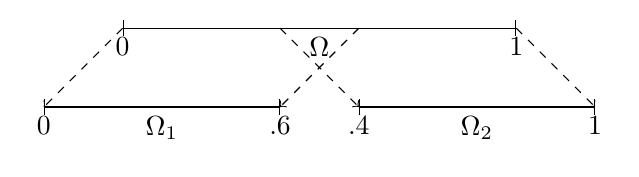
\begin{tikzpicture}
      \draw[|-|] (3,2) -- (8,2)
      node[pos=0, below]{$0$}
      node[pos=.5,below]{$\Omega$}
      node[pos=1, below]{$1$};

      \onslide<2->
      {
      \draw[|-|] (2,1) -- (5,1)
      node[pos=0, below]{$0$}
      node[pos=.5,below]{$\Omega_1$}
      node[pos=1, below]{$.6$};

      \draw[|-|] (6,1) -- (9,1)
      node[pos=0, below]{$.4$}      
      node[pos=.5,below]{$\Omega_2$}
      node[pos=1, below]{$1$};      

      \draw[->,dashed] (5,2) -- (6,1);
      \draw[->,dashed] (8,2) -- (9,1);
      \draw[->,dashed] (6,2) -- (5,1);
      \draw[->,dashed] (3,2) -- (2,1);
      }
    \end{tikzpicture}
  \end{figure}


\end{frame}


\begin{frame}{PDE of interest}{Domain Decomposition}
  
  \begin{eqnarray}
    (u_i)_t =  \mathcal{L}(t,u_i), \quad (x,t)\in \Omega_i\times[0,T]\\
    \nonumber
    u_i(x,0) = f(x), \quad x \in \Omega_i \\
    \nonumber
    u_i(z,t) = g(z,t), \quad z \in \partial\Omega_i\cap\partial\Omega, \\
    \nonumber
    \mathcal{T}_{ij}(u_{i}(z,t)) = \mathcal{T}_{ij}(u_{j}(z,t)), \quad z \in \partial\Omega_i\cap\partial\Omega_j.
  \end{eqnarray}  
\end{frame}


\begin{frame}{Transmission Conditions}

  \begin{itemize}
  \item Choice of transmission conditions crucial for good performance
  \item Overlapping domains
  \item Non-overlapping domains
  \item Optimized transmission conditions
    \[
    \mathcal{T}_{ij}[\cdot] = \left(\frac{d}{d\hat{n}} + p\right) [\cdot], 
    \quad
    \mathcal{T}_{ji}[\cdot] = \left(\frac{d}{d\hat{n}} - p\right) [\cdot],
    \]      
  \end{itemize}
  
\end{frame}


\subsection{Schwarz Waveform Relaxation}

\begin{frame}{Schwarz Iteration}

  \begin{itemize}
  \item Domain Decomposition in space
  \item Discretize in time
  \item High communication cost
  \item Does not naturally handle varying time discretizations
    \begin{itemize}
    \item Difficult to make adaptive in time
    \end{itemize}
  \end{itemize}


\end{frame}


\begin{frame}{Schwarz Waveform Relaxation (SWR)}

  \begin{itemize}
  \item<1-> Domain decomposition in space
  \item<1-> On each subdomain solve for multiple time steps per iteration    
    \begin{itemize}
    \item From $[\Delta t,T]$
    \end{itemize}
  \item<2-> Communicate transmission conditions for many points in one message
  \item<2-> Optimal transmission conditions 
  \item<2-> Active area of research

  \end{itemize}

\end{frame}


\begin{frame}
  \frametitle{Schwarz Waveform Relaxation (animation)}
  \only<1>{
    \begin{figure}
      \centering
       \definecolor{darkgreen}{rgb}{0,.6,0}
  \begin{tikzpicture}[scale=1.0]

    \tikzstyle{dropline_style}=[densely dotted,thin]

    %\foreach \x/\xtext in {-1, -0.5/-\frac{1}{2}, 1}
    %\draw (\x cm,1pt) -- (\x cm,-1pt) node[anchor=north] {$\xtext$};

    \draw(-2,5) node[left] {.};
    \draw (-2.2, 1) node[left] {\small waveform iterate \# 1};
    %\draw (-2.2, 1) node[left] {\small waveform iterate \# 2};
    %\draw (-2.2, 2) node[left] {\small waveform iterate \# 3};
    %\draw (-2.2, 3) node[left] {\small waveform iterate \# 4};
    %\draw (-2.2, 4) node[left] {\small waveform iterate \# 5};

    \def\a{-0.25}
    \def\b{0.5}
    \draw (-1,\a) -- (5,\a);
    \draw (5,\a) -- (5,\b);
    \draw (5,\b) -- (-1,\b);
    \draw (-1,\b) -- (-1,\a);

    \def\c{0.75}
    \def\d{1.5}
    \draw (-1,\c) -- (5,\c);
    \draw (5,\c) -- (5,\d);
    \draw (5,\d) -- (-1,\d);
    \draw (-1,\d) -- (-1,\c);

    \draw(-1,0.1) node[left] {$\Omega_0$};
    \draw(-1,1.15) node[left] {$\Omega_1$};

%\draw (2,0.2) -- (2,-0.2) node[below] {$\alpha$};
%\draw (4,0.2) -- (4,-0.2) node[below] {1};

    % position of the time-line
    \def\y{-0.5}
    \draw [-] (-1,\y) -- (5,\y);

    \def\tick{0.05}
    \draw (-1,\y) ++(0,\tick) -- ++(0,-2*\tick) node[below] {\small $t^{0}$};
    \draw (0,\y) ++(0,\tick) -- ++(0,-2*\tick) node[below] {\small $t^{1}$};
    \draw (1,\y) ++(0,\tick) -- ++(0,-2*\tick) node[below] {\small $t^{2}$};
    \draw (2,\y) ++(0,\tick) -- ++(0,-2*\tick) node[below] {\small $t^{3}$};
    \draw (3,\y) ++(0,\tick) -- ++(0,-2*\tick) node[below] {\small $t^{4}$};
    \draw (4,\y)  node[below] {\small \phantom{t}$\ldots$\phantom{t}};  
    \draw (5,\y) ++(0,\tick) -- ++(0,-2*\tick) node[below] {\small $t^{N}$};
  
    % parameters for stencil diagrams
    \def\rad{0.12}
    \def\omr{0.88}   % 1-rad
    \def\intthick{0.068}   % thickness of integral bars

    % filled dots
    %\foreach \xy in { (-1,0) }
    %\filldraw \xy circle (2pt);

    % hollow dots
    %\foreach \xy in { (0,0)}
    %\filldraw[fill=white] \xy circle (2.5pt);

    % arrows
    %\draw [->,thick,blue] (-1,0.13) arc (160:20:0.5 and 0.5);

  \end{tikzpicture}

    \end{figure}
  }
  \only<2>{
    \begin{figure}
      \centering
       \definecolor{darkgreen}{rgb}{0,.6,0}
  \begin{tikzpicture}[scale=1.0]

    \tikzstyle{dropline_style}=[densely dotted,thin]

    %\foreach \x/\xtext in {-1, -0.5/-\frac{1}{2}, 1}
    %\draw (\x cm,1pt) -- (\x cm,-1pt) node[anchor=north] {$\xtext$};

    \draw(-2,5) node[left] {.};
    \draw (-2.2, 1) node[left] {\small waveform iterate \# 1};
    %\draw (-2.2, 1) node[left] {\small waveform iterate \# 2};
    %\draw (-2.2, 2) node[left] {\small waveform iterate \# 3};
    %\draw (-2.2, 3) node[left] {\small waveform iterate \# 4};
    %\draw (-2.2, 4) node[left] {\small waveform iterate \# 5};

    \def\a{-0.25}
    \def\b{0.5}
    \draw (-1,\a) -- (5,\a);
    \draw (5,\a) -- (5,\b);
    \draw (5,\b) -- (-1,\b);
    \draw (-1,\b) -- (-1,\a);

    \def\c{0.75}
    \def\d{1.5}
    \draw (-1,\c) -- (5,\c);
    \draw (5,\c) -- (5,\d);
    \draw (5,\d) -- (-1,\d);
    \draw (-1,\d) -- (-1,\c);

    \draw(-1,0.1) node[left] {$\Omega_0$};
    \draw(-1,1.15) node[left] {$\Omega_1$};

%\draw (2,0.2) -- (2,-0.2) node[below] {$\alpha$};
%\draw (4,0.2) -- (4,-0.2) node[below] {1};

    % position of the time-line
    \def\y{-0.5}
    \draw [-] (-1,\y) -- (5,\y);

    \def\tick{0.05}
    \draw (-1,\y) ++(0,\tick) -- ++(0,-2*\tick) node[below] {\small $t^{0}$};
    \draw (0,\y) ++(0,\tick) -- ++(0,-2*\tick) node[below] {\small $t^{1}$};
    \draw (1,\y) ++(0,\tick) -- ++(0,-2*\tick) node[below] {\small $t^{2}$};
    \draw (2,\y) ++(0,\tick) -- ++(0,-2*\tick) node[below] {\small $t^{3}$};
    \draw (3,\y) ++(0,\tick) -- ++(0,-2*\tick) node[below] {\small $t^{4}$};
    \draw (4,\y)  node[below] {\small \phantom{t}$\ldots$\phantom{t}};  
    \draw (5,\y) ++(0,\tick) -- ++(0,-2*\tick) node[below] {\small $t^{N}$};
  
    % parameters for stencil diagrams
    \def\rad{0.12}
    \def\omr{0.88}   % 1-rad
    \def\intthick{0.068}   % thickness of integral bars

    % filled dots
    %\foreach \xy in { (-1,0) }
    %\filldraw \xy circle (2pt);

    % hollow dots
    %\foreach \xy in { (0,0)}
    %\filldraw[fill=white] \xy circle (2.5pt);

    % arrows
%    \draw [->,thick,blue] (-1,0) arc (160:20:0.5 and 0.5);
%    \draw [->,thick,blue] (-1,1) arc (160:20:0.5 and 0.5);

    \draw [-latex,thick,blue] (-1,0.2) -- (0,0.2);
    \draw [-latex,thick,blue] (-1,1.2) -- (0,1.2);

    \draw [-,thick,red] (0,\a) -- (0,\b);
    \draw [-,thick,red] (0,\c) -- (0,\d);
  \end{tikzpicture}

    \end{figure}
  }
  \only<3>{
    \begin{figure}
      \centering
       \definecolor{darkgreen}{rgb}{0,.6,0}
  \begin{tikzpicture}[scale=1.0]

    \tikzstyle{dropline_style}=[densely dotted,thin]

    %\foreach \x/\xtext in {-1, -0.5/-\frac{1}{2}, 1}
    %\draw (\x cm,1pt) -- (\x cm,-1pt) node[anchor=north] {$\xtext$};

    \draw(-2,5) node[left] {.};
    \draw (-2.2, 1) node[left] {\small waveform iterate \# 1};
    %\draw (-2.2, 1) node[left] {\small waveform iterate \# 2};
    %\draw (-2.2, 2) node[left] {\small waveform iterate \# 3};
    %\draw (-2.2, 3) node[left] {\small waveform iterate \# 4};
    %\draw (-2.2, 4) node[left] {\small waveform iterate \# 5};

    \def\a{-0.25}
    \def\b{0.5}
    \draw (-1,\a) -- (5,\a);
    \draw (5,\a) -- (5,\b);
    \draw (5,\b) -- (-1,\b);
    \draw (-1,\b) -- (-1,\a);

    \def\c{0.75}
    \def\d{1.5}
    \draw (-1,\c) -- (5,\c);
    \draw (5,\c) -- (5,\d);
    \draw (5,\d) -- (-1,\d);
    \draw (-1,\d) -- (-1,\c);

    \draw(-1,0.1) node[left] {$\Omega_0$};
    \draw(-1,1.15) node[left] {$\Omega_1$};

%\draw (2,0.2) -- (2,-0.2) node[below] {$\alpha$};
%\draw (4,0.2) -- (4,-0.2) node[below] {1};

    % position of the time-line
    \def\y{-0.5}
    \draw [-] (-1,\y) -- (5,\y);

    \def\tick{0.05}
    \draw (-1,\y) ++(0,\tick) -- ++(0,-2*\tick) node[below] {\small $t^{0}$};
    \draw (0,\y) ++(0,\tick) -- ++(0,-2*\tick) node[below] {\small $t^{1}$};
    \draw (1,\y) ++(0,\tick) -- ++(0,-2*\tick) node[below] {\small $t^{2}$};
    \draw (2,\y) ++(0,\tick) -- ++(0,-2*\tick) node[below] {\small $t^{3}$};
    \draw (3,\y) ++(0,\tick) -- ++(0,-2*\tick) node[below] {\small $t^{4}$};
    \draw (4,\y)  node[below] {\small \phantom{t}$\ldots$\phantom{t}};  
    \draw (5,\y) ++(0,\tick) -- ++(0,-2*\tick) node[below] {\small $t^{N}$};
  
    % parameters for stencil diagrams
    \def\rad{0.12}
    \def\omr{0.88}   % 1-rad
    \def\intthick{0.068}   % thickness of integral bars

    % filled dots
    %\foreach \xy in { (-1,0) }
    %\filldraw \xy circle (2pt);

    % hollow dots
    %\foreach \xy in { (0,0)}
    %\filldraw[fill=white] \xy circle (2.5pt);

    % arrows
%    \draw [->,thick,blue] (-1,0) arc (160:20:0.5 and 0.5);
%    \draw [->,thick,blue] (-1,1) arc (160:20:0.5 and 0.5);

%    \draw [-latex,thick,blue] (-1,0.2) -- (0,0.2);
%    \draw [-latex,thick,blue] (-1,1.2) -- (0,1.2);

    \draw [-,thick,black] (0,\a) -- (0,\b);
    \draw [-,thick,black] (0,\c) -- (0,\d);
  \end{tikzpicture}

    \end{figure}
  }
  \only<4>{
    \begin{figure}
      \centering
       \definecolor{darkgreen}{rgb}{0,.6,0}
  \begin{tikzpicture}[scale=1.0]

    \tikzstyle{dropline_style}=[densely dotted,thin]

    %\foreach \x/\xtext in {-1, -0.5/-\frac{1}{2}, 1}
    %\draw (\x cm,1pt) -- (\x cm,-1pt) node[anchor=north] {$\xtext$};

    \draw(-2,5) node[left] {.};
    \draw (-2.2, 1) node[left] {\small waveform iterate \# 1};
    %\draw (-2.2, 1) node[left] {\small waveform iterate \# 2};
    %\draw (-2.2, 2) node[left] {\small waveform iterate \# 3};
    %\draw (-2.2, 3) node[left] {\small waveform iterate \# 4};
    %\draw (-2.2, 4) node[left] {\small waveform iterate \# 5};

    \def\a{-0.25}
    \def\b{0.5}
    \draw (-1,\a) -- (5,\a);
    \draw (5,\a) -- (5,\b);
    \draw (5,\b) -- (-1,\b);
    \draw (-1,\b) -- (-1,\a);

    \def\c{0.75}
    \def\d{1.5}
    \draw (-1,\c) -- (5,\c);
    \draw (5,\c) -- (5,\d);
    \draw (5,\d) -- (-1,\d);
    \draw (-1,\d) -- (-1,\c);

    \draw(-1,0.1) node[left] {$\Omega_0$};
    \draw(-1,1.15) node[left] {$\Omega_1$};

%\draw (2,0.2) -- (2,-0.2) node[below] {$\alpha$};
%\draw (4,0.2) -- (4,-0.2) node[below] {1};

    % position of the time-line
    \def\y{-0.5}
    \draw [-] (-1,\y) -- (5,\y);

    \def\tick{0.05}
    \draw (-1,\y) ++(0,\tick) -- ++(0,-2*\tick) node[below] {\small $t^{0}$};
    \draw (0,\y) ++(0,\tick) -- ++(0,-2*\tick) node[below] {\small $t^{1}$};
    \draw (1,\y) ++(0,\tick) -- ++(0,-2*\tick) node[below] {\small $t^{2}$};
    \draw (2,\y) ++(0,\tick) -- ++(0,-2*\tick) node[below] {\small $t^{3}$};
    \draw (3,\y) ++(0,\tick) -- ++(0,-2*\tick) node[below] {\small $t^{4}$};
    \draw (4,\y)  node[below] {\small \phantom{t}$\ldots$\phantom{t}};  
    \draw (5,\y) ++(0,\tick) -- ++(0,-2*\tick) node[below] {\small $t^{N}$};
  
    % parameters for stencil diagrams
    \def\rad{0.12}
    \def\omr{0.88}   % 1-rad
    \def\intthick{0.068}   % thickness of integral bars

    % filled dots
    %\foreach \xy in { (-1,0) }
    %\filldraw \xy circle (2pt);

    % hollow dots
    %\foreach \xy in { (0,0)}
    %\filldraw[fill=white] \xy circle (2.5pt);

    \draw [-latex,thick,blue] (0,0.2) -- (1,0.2);
    \draw [-latex,thick,blue] (0,1.2) -- (1,1.2);

    \draw [-,thick,black] (0,\a) -- (0,\b);
    \draw [-,thick,black] (0,\c) -- (0,\d);

    \draw [-,thick,red] (1,\a) -- (1,\b);
    \draw [-,thick,red] (1,\c) -- (1,\d);
  \end{tikzpicture}

    \end{figure}
  }
  \only<5>{
    \begin{figure}
      \centering
       \definecolor{darkgreen}{rgb}{0,.6,0}
  \begin{tikzpicture}[scale=1.0]

    \tikzstyle{dropline_style}=[densely dotted,thin]

    %\foreach \x/\xtext in {-1, -0.5/-\frac{1}{2}, 1}
    %\draw (\x cm,1pt) -- (\x cm,-1pt) node[anchor=north] {$\xtext$};

    \draw(-2,5) node[left] {.};
    \draw (-2.2, 1) node[left] {\small waveform iterate \# 1};
    %\draw (-2.2, 1) node[left] {\small waveform iterate \# 2};
    %\draw (-2.2, 2) node[left] {\small waveform iterate \# 3};
    %\draw (-2.2, 3) node[left] {\small waveform iterate \# 4};
    %\draw (-2.2, 4) node[left] {\small waveform iterate \# 5};

    \def\a{-0.25}
    \def\b{0.5}
    \draw (-1,\a) -- (5,\a);
    \draw (5,\a) -- (5,\b);
    \draw (5,\b) -- (-1,\b);
    \draw (-1,\b) -- (-1,\a);

    \def\c{0.75}
    \def\d{1.5}
    \draw (-1,\c) -- (5,\c);
    \draw (5,\c) -- (5,\d);
    \draw (5,\d) -- (-1,\d);
    \draw (-1,\d) -- (-1,\c);

    \draw(-1,0.1) node[left] {$\Omega_0$};
    \draw(-1,1.15) node[left] {$\Omega_1$};

%\draw (2,0.2) -- (2,-0.2) node[below] {$\alpha$};
%\draw (4,0.2) -- (4,-0.2) node[below] {1};

    % position of the time-line
    \def\y{-0.5}
    \draw [-] (-1,\y) -- (5,\y);

    \def\tick{0.05}
    \draw (-1,\y) ++(0,\tick) -- ++(0,-2*\tick) node[below] {\small $t^{0}$};
    \draw (0,\y) ++(0,\tick) -- ++(0,-2*\tick) node[below] {\small $t^{1}$};
    \draw (1,\y) ++(0,\tick) -- ++(0,-2*\tick) node[below] {\small $t^{2}$};
    \draw (2,\y) ++(0,\tick) -- ++(0,-2*\tick) node[below] {\small $t^{3}$};
    \draw (3,\y) ++(0,\tick) -- ++(0,-2*\tick) node[below] {\small $t^{4}$};
    \draw (4,\y)  node[below] {\small \phantom{t}$\ldots$\phantom{t}};  
    \draw (5,\y) ++(0,\tick) -- ++(0,-2*\tick) node[below] {\small $t^{N}$};
  
    % parameters for stencil diagrams
    \def\rad{0.12}
    \def\omr{0.88}   % 1-rad
    \def\intthick{0.068}   % thickness of integral bars

    % filled dots
    %\foreach \xy in { (-1,0) }
    %\filldraw \xy circle (2pt);

    % hollow dots
    %\foreach \xy in { (0,0)}
    %\filldraw[fill=white] \xy circle (2.5pt);

    %\draw [-latex,thick,blue] (0,0.2) -- (1,0.2);
    %\draw [-latex,thick,blue] (0,1.2) -- (1,1.2);

    \draw [-,thick,black] (0,\a) -- (0,\b);
    \draw [-,thick,black] (0,\c) -- (0,\d);

    \draw [-,thick,black] (1,\a) -- (1,\b);
    \draw [-,thick,black] (1,\c) -- (1,\d);
  \end{tikzpicture}

    \end{figure}
  }
  \only<6>{
    \begin{figure}
      \centering
       \definecolor{darkgreen}{rgb}{0,.6,0}
  \begin{tikzpicture}[scale=1.0]

    \tikzstyle{dropline_style}=[densely dotted,thin]

    %\foreach \x/\xtext in {-1, -0.5/-\frac{1}{2}, 1}
    %\draw (\x cm,1pt) -- (\x cm,-1pt) node[anchor=north] {$\xtext$};

    \draw(-2,5) node[left] {.};
    \draw (-2.2, 1) node[left] {\small waveform iterate \# 1};
    %\draw (-2.2, 1) node[left] {\small waveform iterate \# 2};
    %\draw (-2.2, 2) node[left] {\small waveform iterate \# 3};
    %\draw (-2.2, 3) node[left] {\small waveform iterate \# 4};
    %\draw (-2.2, 4) node[left] {\small waveform iterate \# 5};

    \def\a{-0.25}
    \def\b{0.5}
    \draw (-1,\a) -- (5,\a);
    \draw (5,\a) -- (5,\b);
    \draw (5,\b) -- (-1,\b);
    \draw (-1,\b) -- (-1,\a);

    \def\c{0.75}
    \def\d{1.5}
    \draw (-1,\c) -- (5,\c);
    \draw (5,\c) -- (5,\d);
    \draw (5,\d) -- (-1,\d);
    \draw (-1,\d) -- (-1,\c);

    \draw(-1,0.1) node[left] {$\Omega_0$};
    \draw(-1,1.15) node[left] {$\Omega_1$};

%\draw (2,0.2) -- (2,-0.2) node[below] {$\alpha$};
%\draw (4,0.2) -- (4,-0.2) node[below] {1};

    % position of the time-line
    \def\y{-0.5}
    \draw [-] (-1,\y) -- (5,\y);

    \def\tick{0.05}
    \draw (-1,\y) ++(0,\tick) -- ++(0,-2*\tick) node[below] {\small $t^{0}$};
    \draw (0,\y) ++(0,\tick) -- ++(0,-2*\tick) node[below] {\small $t^{1}$};
    \draw (1,\y) ++(0,\tick) -- ++(0,-2*\tick) node[below] {\small $t^{2}$};
    \draw (2,\y) ++(0,\tick) -- ++(0,-2*\tick) node[below] {\small $t^{3}$};
    \draw (3,\y) ++(0,\tick) -- ++(0,-2*\tick) node[below] {\small $t^{4}$};
    \draw (4,\y)  node[below] {\small \phantom{t}$\ldots$\phantom{t}};  
    \draw (5,\y) ++(0,\tick) -- ++(0,-2*\tick) node[below] {\small $t^{N}$};
  
    % parameters for stencil diagrams
    \def\rad{0.12}
    \def\omr{0.88}   % 1-rad
    \def\intthick{0.068}   % thickness of integral bars

    % filled dots
    %\foreach \xy in { (-1,0) }
    %\filldraw \xy circle (2pt);

    % hollow dots
    %\foreach \xy in { (0,0)}
    %\filldraw[fill=white] \xy circle (2.5pt);

    \draw [-latex,thick,blue] (1,0.2) -- (2,0.2);
    \draw [-latex,thick,blue] (1,1.2) -- (2,1.2);

    \draw [-,thick,black] (0,\a) -- (0,\b);
    \draw [-,thick,black] (0,\c) -- (0,\d);

    \draw [-,thick,black] (1,\a) -- (1,\b);
    \draw [-,thick,black] (1,\c) -- (1,\d);

    \draw [-,thick,red] (2,\a) -- (2,\b);
    \draw [-,thick,red] (2,\c) -- (2,\d);
  \end{tikzpicture}

    \end{figure}
  }
  \only<7>{
    \begin{figure}
      \centering
       \definecolor{darkgreen}{rgb}{0,.6,0}
  \begin{tikzpicture}[scale=1.0]

    \tikzstyle{dropline_style}=[densely dotted,thin]

    %\foreach \x/\xtext in {-1, -0.5/-\frac{1}{2}, 1}
    %\draw (\x cm,1pt) -- (\x cm,-1pt) node[anchor=north] {$\xtext$};

    \draw(-2,5) node[left] {.};
    \draw (-2.2, 1) node[left] {\small waveform iterate \# 1};
    %\draw (-2.2, 1) node[left] {\small waveform iterate \# 2};
    %\draw (-2.2, 2) node[left] {\small waveform iterate \# 3};
    %\draw (-2.2, 3) node[left] {\small waveform iterate \# 4};
    %\draw (-2.2, 4) node[left] {\small waveform iterate \# 5};

    \def\a{-0.25}
    \def\b{0.5}
    \draw (-1,\a) -- (5,\a);
    \draw (5,\a) -- (5,\b);
    \draw (5,\b) -- (-1,\b);
    \draw (-1,\b) -- (-1,\a);

    \def\c{0.75}
    \def\d{1.5}
    \draw (-1,\c) -- (5,\c);
    \draw (5,\c) -- (5,\d);
    \draw (5,\d) -- (-1,\d);
    \draw (-1,\d) -- (-1,\c);

    \draw(-1,0.1) node[left] {$\Omega_0$};
    \draw(-1,1.15) node[left] {$\Omega_1$};

%\draw (2,0.2) -- (2,-0.2) node[below] {$\alpha$};
%\draw (4,0.2) -- (4,-0.2) node[below] {1};

    % position of the time-line
    \def\y{-0.5}
    \draw [-] (-1,\y) -- (5,\y);

    \def\tick{0.05}
    \draw (-1,\y) ++(0,\tick) -- ++(0,-2*\tick) node[below] {\small $t^{0}$};
    \draw (0,\y) ++(0,\tick) -- ++(0,-2*\tick) node[below] {\small $t^{1}$};
    \draw (1,\y) ++(0,\tick) -- ++(0,-2*\tick) node[below] {\small $t^{2}$};
    \draw (2,\y) ++(0,\tick) -- ++(0,-2*\tick) node[below] {\small $t^{3}$};
    \draw (3,\y) ++(0,\tick) -- ++(0,-2*\tick) node[below] {\small $t^{4}$};
    \draw (4,\y)  node[below] {\small \phantom{t}$\ldots$\phantom{t}};  
    \draw (5,\y) ++(0,\tick) -- ++(0,-2*\tick) node[below] {\small $t^{N}$};
  
    % parameters for stencil diagrams
    \def\rad{0.12}
    \def\omr{0.88}   % 1-rad
    \def\intthick{0.068}   % thickness of integral bars

    % filled dots
    %\foreach \xy in { (-1,0) }
    %\filldraw \xy circle (2pt);

    % hollow dots
    %\foreach \xy in { (0,0)}
    %\filldraw[fill=white] \xy circle (2.5pt);

    %\draw [-latex,thick,blue] (1,0.2) -- (2,0.2);
    %\draw [-latex,thick,blue] (1,1.2) -- (2,1.2);

    \draw [-,thick,black] (0,\a) -- (0,\b);
    \draw [-,thick,black] (0,\c) -- (0,\d);

    \draw [-,thick,black] (1,\a) -- (1,\b);
    \draw [-,thick,black] (1,\c) -- (1,\d);

    \draw [-,thick,black] (2,\a) -- (2,\b);
    \draw [-,thick,black] (2,\c) -- (2,\d);
  \end{tikzpicture}

    \end{figure}
  }
  \only<8>{
    \begin{figure}
      \centering
       \definecolor{darkgreen}{rgb}{0,.6,0}
  \begin{tikzpicture}[scale=1.0]

    \tikzstyle{dropline_style}=[densely dotted,thin]

    %\foreach \x/\xtext in {-1, -0.5/-\frac{1}{2}, 1}
    %\draw (\x cm,1pt) -- (\x cm,-1pt) node[anchor=north] {$\xtext$};

    \draw(-2,5) node[left] {.};
    \draw (-2.2, 1) node[left] {\small waveform iterate \# 1};
    %\draw (-2.2, 1) node[left] {\small waveform iterate \# 2};
    %\draw (-2.2, 2) node[left] {\small waveform iterate \# 3};
    %\draw (-2.2, 3) node[left] {\small waveform iterate \# 4};
    %\draw (-2.2, 4) node[left] {\small waveform iterate \# 5};

    \def\a{-0.25}
    \def\b{0.5}
    \draw (-1,\a) -- (5,\a);
    \draw (5,\a) -- (5,\b);
    \draw (5,\b) -- (-1,\b);
    \draw (-1,\b) -- (-1,\a);

    \def\c{0.75}
    \def\d{1.5}
    \draw (-1,\c) -- (5,\c);
    \draw (5,\c) -- (5,\d);
    \draw (5,\d) -- (-1,\d);
    \draw (-1,\d) -- (-1,\c);

    \draw(-1,0.1) node[left] {$\Omega_0$};
    \draw(-1,1.15) node[left] {$\Omega_1$};

%\draw (2,0.2) -- (2,-0.2) node[below] {$\alpha$};
%\draw (4,0.2) -- (4,-0.2) node[below] {1};

    % position of the time-line
    \def\y{-0.5}
    \draw [-] (-1,\y) -- (5,\y);

    \def\tick{0.05}
    \draw (-1,\y) ++(0,\tick) -- ++(0,-2*\tick) node[below] {\small $t^{0}$};
    \draw (0,\y) ++(0,\tick) -- ++(0,-2*\tick) node[below] {\small $t^{1}$};
    \draw (1,\y) ++(0,\tick) -- ++(0,-2*\tick) node[below] {\small $t^{2}$};
    \draw (2,\y) ++(0,\tick) -- ++(0,-2*\tick) node[below] {\small $t^{3}$};
    \draw (3,\y) ++(0,\tick) -- ++(0,-2*\tick) node[below] {\small $t^{4}$};
    \draw (4,\y)  node[below] {\small \phantom{t}$\ldots$\phantom{t}};  
    \draw (5,\y) ++(0,\tick) -- ++(0,-2*\tick) node[below] {\small $t^{N}$};
  
    % parameters for stencil diagrams
    \def\rad{0.12}
    \def\omr{0.88}   % 1-rad
    \def\intthick{0.068}   % thickness of integral bars

    % filled dots
    %\foreach \xy in { (-1,0) }
    %\filldraw \xy circle (2pt);

    % hollow dots
    %\foreach \xy in { (0,0)}
    %\filldraw[fill=white] \xy circle (2.5pt);

    \draw [-latex,thick,blue] (2,0.2) -- (3,0.2);
    \draw [-latex,thick,blue] (2,1.2) -- (3,1.2);

    \draw [-,thick,black] (0,\a) -- (0,\b);
    \draw [-,thick,black] (0,\c) -- (0,\d);

    \draw [-,thick,black] (1,\a) -- (1,\b);
    \draw [-,thick,black] (1,\c) -- (1,\d);

    \draw [-,thick,black] (2,\a) -- (2,\b);
    \draw [-,thick,black] (2,\c) -- (2,\d);

    \draw [-,thick,red] (3,\a) -- (3,\b);
    \draw [-,thick,red] (3,\c) -- (3,\d);
  \end{tikzpicture}

    \end{figure}
  }
  \only<9>{
    \begin{figure}
      \centering
       \definecolor{darkgreen}{rgb}{0,.6,0}
  \begin{tikzpicture}[scale=1.0]

    \tikzstyle{dropline_style}=[densely dotted,thin]

    %\foreach \x/\xtext in {-1, -0.5/-\frac{1}{2}, 1}
    %\draw (\x cm,1pt) -- (\x cm,-1pt) node[anchor=north] {$\xtext$};

    \draw(-2,5) node[left] {.};
    \draw (-2.2, 1) node[left] {\small waveform iterate \# 1};
    %\draw (-2.2, 1) node[left] {\small waveform iterate \# 2};
    %\draw (-2.2, 2) node[left] {\small waveform iterate \# 3};
    %\draw (-2.2, 3) node[left] {\small waveform iterate \# 4};
    %\draw (-2.2, 4) node[left] {\small waveform iterate \# 5};

    \def\a{-0.25}
    \def\b{0.5}
    \draw (-1,\a) -- (5,\a);
    \draw (5,\a) -- (5,\b);
    \draw (5,\b) -- (-1,\b);
    \draw (-1,\b) -- (-1,\a);

    \def\c{0.75}
    \def\d{1.5}
    \draw (-1,\c) -- (5,\c);
    \draw (5,\c) -- (5,\d);
    \draw (5,\d) -- (-1,\d);
    \draw (-1,\d) -- (-1,\c);

    \draw(-1,0.1) node[left] {$\Omega_0$};
    \draw(-1,1.15) node[left] {$\Omega_1$};

%\draw (2,0.2) -- (2,-0.2) node[below] {$\alpha$};
%\draw (4,0.2) -- (4,-0.2) node[below] {1};

    % position of the time-line
    \def\y{-0.5}
    \draw [-] (-1,\y) -- (5,\y);

    \def\tick{0.05}
    \draw (-1,\y) ++(0,\tick) -- ++(0,-2*\tick) node[below] {\small $t^{0}$};
    \draw (0,\y) ++(0,\tick) -- ++(0,-2*\tick) node[below] {\small $t^{1}$};
    \draw (1,\y) ++(0,\tick) -- ++(0,-2*\tick) node[below] {\small $t^{2}$};
    \draw (2,\y) ++(0,\tick) -- ++(0,-2*\tick) node[below] {\small $t^{3}$};
    \draw (3,\y) ++(0,\tick) -- ++(0,-2*\tick) node[below] {\small $t^{4}$};
    \draw (4,\y)  node[below] {\small \phantom{t}$\ldots$\phantom{t}};  
    \draw (5,\y) ++(0,\tick) -- ++(0,-2*\tick) node[below] {\small $t^{N}$};
  
    % parameters for stencil diagrams
    \def\rad{0.12}
    \def\omr{0.88}   % 1-rad
    \def\intthick{0.068}   % thickness of integral bars

    % filled dots
    %\foreach \xy in { (-1,0) }
    %\filldraw \xy circle (2pt);

    % hollow dots
    %\foreach \xy in { (0,0)}
    %\filldraw[fill=white] \xy circle (2.5pt);

    %\draw [-latex,thick,blue] (2,0.2) -- (3,0.2);
    %\draw [-latex,thick,blue] (2,1.2) -- (3,1.2);

    \draw [-,thick,black] (0,\a) -- (0,\b);
    \draw [-,thick,black] (0,\c) -- (0,\d);

    \draw [-,thick,black] (1,\a) -- (1,\b);
    \draw [-,thick,black] (1,\c) -- (1,\d);

    \draw [-,thick,black] (2,\a) -- (2,\b);
    \draw [-,thick,black] (2,\c) -- (2,\d);

    \draw [-,thick,black] (3,\a) -- (3,\b);
    \draw [-,thick,black] (3,\c) -- (3,\d);
  \end{tikzpicture}

    \end{figure}
  }
  \only<10>{
    \begin{figure}
      \centering
       \definecolor{darkgreen}{rgb}{0,.6,0}
  \begin{tikzpicture}[scale=1.0]

    \tikzstyle{dropline_style}=[densely dotted,thin]

    %\foreach \x/\xtext in {-1, -0.5/-\frac{1}{2}, 1}
    %\draw (\x cm,1pt) -- (\x cm,-1pt) node[anchor=north] {$\xtext$};

    \draw(-2,5) node[left] {.};
    \draw (-2.2, 1) node[left] {\small waveform iterate \# 1};
    %\draw (-2.2, 1) node[left] {\small waveform iterate \# 2};
    %\draw (-2.2, 2) node[left] {\small waveform iterate \# 3};
    %\draw (-2.2, 3) node[left] {\small waveform iterate \# 4};
    %\draw (-2.2, 4) node[left] {\small waveform iterate \# 5};

    \def\a{-0.25}
    \def\b{0.5}
    \draw (-1,\a) -- (5,\a);
    \draw (5,\a) -- (5,\b);
    \draw (5,\b) -- (-1,\b);
    \draw (-1,\b) -- (-1,\a);

    \def\c{0.75}
    \def\d{1.5}
    \draw (-1,\c) -- (5,\c);
    \draw (5,\c) -- (5,\d);
    \draw (5,\d) -- (-1,\d);
    \draw (-1,\d) -- (-1,\c);

    \draw(-1,0.1) node[left] {$\Omega_0$};
    \draw(-1,1.15) node[left] {$\Omega_1$};

%\draw (2,0.2) -- (2,-0.2) node[below] {$\alpha$};
%\draw (4,0.2) -- (4,-0.2) node[below] {1};

    % position of the time-line
    \def\y{-0.5}
    \draw [-] (-1,\y) -- (5,\y);

    \def\tick{0.05}
    \draw (-1,\y) ++(0,\tick) -- ++(0,-2*\tick) node[below] {\small $t^{0}$};
    \draw (0,\y) ++(0,\tick) -- ++(0,-2*\tick) node[below] {\small $t^{1}$};
    \draw (1,\y) ++(0,\tick) -- ++(0,-2*\tick) node[below] {\small $t^{2}$};
    \draw (2,\y) ++(0,\tick) -- ++(0,-2*\tick) node[below] {\small $t^{3}$};
    \draw (3,\y) ++(0,\tick) -- ++(0,-2*\tick) node[below] {\small $t^{4}$};
    \draw (4,\y)  node[below] {\small \phantom{t}$\ldots$\phantom{t}};  
    \draw (5,\y) ++(0,\tick) -- ++(0,-2*\tick) node[below] {\small $t^{N}$};
  
    % parameters for stencil diagrams
    \def\rad{0.12}
    \def\omr{0.88}   % 1-rad
    \def\intthick{0.068}   % thickness of integral bars

    % filled dots
    %\foreach \xy in { (-1,0) }
    %\filldraw \xy circle (2pt);

    % hollow dots
    %\foreach \xy in { (0,0)}
    %\filldraw[fill=white] \xy circle (2.5pt);

    %\draw [-latex,thick,blue] (2,0.2) -- (3,0.2);
    %\draw [-latex,thick,blue] (2,1.2) -- (3,1.2);

    \draw [-,thick,black] (0,\a) -- (0,\b);
    \draw [-,thick,black] (0,\c) -- (0,\d);

    \draw [-,thick,black] (1,\a) -- (1,\b);
    \draw [-,thick,black] (1,\c) -- (1,\d);

    \draw [-,thick,black] (2,\a) -- (2,\b);
    \draw [-,thick,black] (2,\c) -- (2,\d);

    \draw [-,thick,black] (3,\a) -- (3,\b);
    \draw [-,thick,black] (3,\c) -- (3,\d);

    \draw (4,0.45)  node[below] {\small \phantom{t}$\ldots$\phantom{t}};  
    \draw (4,1.45)  node[below] {\small \phantom{t}$\ldots$\phantom{t}};  
    
  \end{tikzpicture}

    \end{figure}
  }
  \only<11>{
    \begin{figure}
      \centering
       \definecolor{darkgreen}{rgb}{0,.6,0}
  \begin{tikzpicture}[scale=1.0]

    \tikzstyle{dropline_style}=[densely dotted,thin]

    %\foreach \x/\xtext in {-1, -0.5/-\frac{1}{2}, 1}
    %\draw (\x cm,1pt) -- (\x cm,-1pt) node[anchor=north] {$\xtext$};

    \draw(-2,5) node[left] {.};
    \draw (-2.2, 1) node[left] {\small waveform iterate \# 1};
    %\draw (-2.2, 1) node[left] {\small waveform iterate \# 2};
    %\draw (-2.2, 2) node[left] {\small waveform iterate \# 3};
    %\draw (-2.2, 3) node[left] {\small waveform iterate \# 4};
    %\draw (-2.2, 4) node[left] {\small waveform iterate \# 5};

    \def\a{-0.25}
    \def\b{0.5}
    \draw (-1,\a) -- (5,\a);
    \draw (5,\a) -- (5,\b);
    \draw (5,\b) -- (-1,\b);
    \draw (-1,\b) -- (-1,\a);

    \def\c{0.75}
    \def\d{1.5}
    \draw (-1,\c) -- (5,\c);
    \draw (5,\c) -- (5,\d);
    \draw (5,\d) -- (-1,\d);
    \draw (-1,\d) -- (-1,\c);

    \draw(-1,0.1) node[left] {$\Omega_0$};
    \draw(-1,1.15) node[left] {$\Omega_1$};

%\draw (2,0.2) -- (2,-0.2) node[below] {$\alpha$};
%\draw (4,0.2) -- (4,-0.2) node[below] {1};

    % position of the time-line
    \def\y{-0.5}
    \draw [-] (-1,\y) -- (5,\y);

    \def\tick{0.05}
    \draw (-1,\y) ++(0,\tick) -- ++(0,-2*\tick) node[below] {\small $t^{0}$};
    \draw (0,\y) ++(0,\tick) -- ++(0,-2*\tick) node[below] {\small $t^{1}$};
    \draw (1,\y) ++(0,\tick) -- ++(0,-2*\tick) node[below] {\small $t^{2}$};
    \draw (2,\y) ++(0,\tick) -- ++(0,-2*\tick) node[below] {\small $t^{3}$};
    \draw (3,\y) ++(0,\tick) -- ++(0,-2*\tick) node[below] {\small $t^{4}$};
    \draw (4,\y)  node[below] {\small \phantom{t}$\ldots$\phantom{t}};  
    \draw (5,\y) ++(0,\tick) -- ++(0,-2*\tick) node[below] {\small $t^{N}$};
  
    % parameters for stencil diagrams
    \def\rad{0.12}
    \def\omr{0.88}   % 1-rad
    \def\intthick{0.068}   % thickness of integral bars


    % hollow dots
    %\foreach \xy in { (0,0)}
    %\filldraw[fill=white] \xy circle (2.5pt);

    %\draw [-latex,thick,blue] (2,0.2) -- (3,0.2);
    %\draw [-latex,thick,blue] (2,1.2) -- (3,1.2);

    \draw [-,thick,black] (0,\a) -- (0,\b);
    \draw [-,thick,black] (0,\c) -- (0,\d);

    \draw [-,thick,black] (1,\a) -- (1,\b);
    \draw [-,thick,black] (1,\c) -- (1,\d);

    \draw [-,thick,black] (2,\a) -- (2,\b);
    \draw [-,thick,black] (2,\c) -- (2,\d);

    \draw [-,thick,black] (3,\a) -- (3,\b);
    \draw [-,thick,black] (3,\c) -- (3,\d);

    \draw (4,0.45)  node[below] {\small \phantom{t}$\ldots$\phantom{t}};  
    \draw (4,1.45)  node[below] {\small \phantom{t}$\ldots$\phantom{t}};  
    

    % filled dots
    \foreach \xy in { (-1,\b),(0,\b),(1,\b),(2,\b),(3,\b),(5,\b)}
    \filldraw [red] \xy circle (2pt);

    \foreach \xy in { (-1,\c),(0,\c),(1,\c),(2,\c),(3,\c),(5,\c)}
    \filldraw [blue] \xy circle (2pt);

    \draw [->,thick,red] (-1.2,0.3) arc (250:110:0.3 and 0.3);
    \draw [->,thick,blue] (5.2,0.9) arc (70:-70:0.3 and 0.3);

  \end{tikzpicture}

    \end{figure}
  }
  \only<12>{
    \begin{figure}
      \centering
       \definecolor{darkgreen}{rgb}{0,.6,0}
  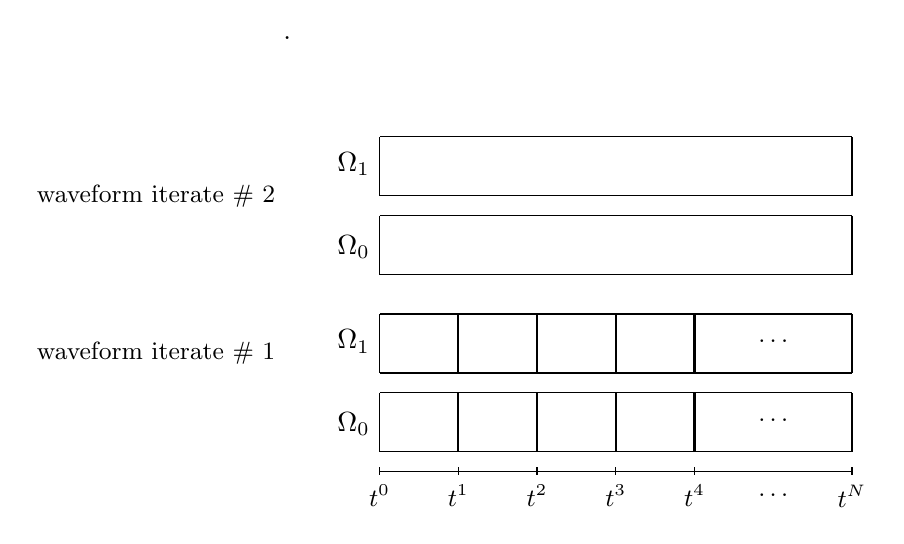
\begin{tikzpicture}[scale=1.0]

    \tikzstyle{dropline_style}=[densely dotted,thin]

    %\foreach \x/\xtext in {-1, -0.5/-\frac{1}{2}, 1}
    %\draw (\x cm,1pt) -- (\x cm,-1pt) node[anchor=north] {$\xtext$};

    \draw(-2,5) node[left] {.};
    \draw (-2.2, 1) node[left] {\small waveform iterate \# 1};
    \draw (-2.2, 3) node[left] {\small waveform iterate \# 2};
    %\draw (-2.2, 2) node[left] {\small waveform iterate \# 3};
    %\draw (-2.2, 3) node[left] {\small waveform iterate \# 4};
    %\draw (-2.2, 4) node[left] {\small waveform iterate \# 5};

    \def\a{-0.25}
    \def\b{0.5}
    \draw (-1,\a) -- (5,\a);
    \draw (5,\a) -- (5,\b);
    \draw (5,\b) -- (-1,\b);
    \draw (-1,\b) -- (-1,\a);

    \def\c{0.75}
    \def\d{1.5}
    \draw (-1,\c) -- (5,\c);
    \draw (5,\c) -- (5,\d);
    \draw (5,\d) -- (-1,\d);
    \draw (-1,\d) -- (-1,\c);

    \draw(-1,0.1) node[left] {$\Omega_0$};
    \draw(-1,1.15) node[left] {$\Omega_1$};

    \def\e{2}
    \def\f{2.75}
    \draw (-1,\e) -- (5,\e);
    \draw (5,\e) -- (5,\f);
    \draw (5,\f) -- (-1,\f);
    \draw (-1,\f) -- (-1,\e);

    \def\g{3}
    \def\h{3.75}
    \draw (-1,\g) -- (5,\g);
    \draw (5,\g) -- (5,\h);
    \draw (5,\h) -- (-1,\h);
    \draw (-1,\h) -- (-1,\g);

    \draw(-1,2.35) node[left] {$\Omega_0$};
    \draw(-1,3.4) node[left] {$\Omega_1$};

%\draw (2,0.2) -- (2,-0.2) node[below] {$\alpha$};
%\draw (4,0.2) -- (4,-0.2) node[below] {1};

    % position of the time-line
    \def\y{-0.5}
    \draw [-] (-1,\y) -- (5,\y);

    \def\tick{0.05}
    \draw (-1,\y) ++(0,\tick) -- ++(0,-2*\tick) node[below] {\small $t^{0}$};
    \draw (0,\y) ++(0,\tick) -- ++(0,-2*\tick) node[below] {\small $t^{1}$};
    \draw (1,\y) ++(0,\tick) -- ++(0,-2*\tick) node[below] {\small $t^{2}$};
    \draw (2,\y) ++(0,\tick) -- ++(0,-2*\tick) node[below] {\small $t^{3}$};
    \draw (3,\y) ++(0,\tick) -- ++(0,-2*\tick) node[below] {\small $t^{4}$};
    \draw (4,\y)  node[below] {\small \phantom{t}$\ldots$\phantom{t}};  
    \draw (5,\y) ++(0,\tick) -- ++(0,-2*\tick) node[below] {\small $t^{N}$};
  
    % parameters for stencil diagrams
    \def\rad{0.12}
    \def\omr{0.88}   % 1-rad
    \def\intthick{0.068}   % thickness of integral bars

    % filled dots
    %\foreach \xy in { (-1,0) }
    %\filldraw \xy circle (2pt);

    % hollow dots
    %\foreach \xy in { (0,0)}
    %\filldraw[fill=white] \xy circle (2.5pt);

    %\draw [-latex,thick,blue] (2,0.2) -- (3,0.2);
    %\draw [-latex,thick,blue] (2,1.2) -- (3,1.2);

    \draw [-,thick,black] (0,\a) -- (0,\b);
    \draw [-,thick,black] (0,\c) -- (0,\d);

    \draw [-,thick,black] (1,\a) -- (1,\b);
    \draw [-,thick,black] (1,\c) -- (1,\d);

    \draw [-,thick,black] (2,\a) -- (2,\b);
    \draw [-,thick,black] (2,\c) -- (2,\d);

    \draw [-,thick,black] (3,\a) -- (3,\b);
    \draw [-,thick,black] (3,\c) -- (3,\d);

    \draw (4,0.45)  node[below] {\small \phantom{t}$\ldots$\phantom{t}};  
    \draw (4,1.45)  node[below] {\small \phantom{t}$\ldots$\phantom{t}};  
    
  \end{tikzpicture}

    \end{figure}
  }
  \only<13>{
    \begin{figure}
      \centering
       \definecolor{darkgreen}{rgb}{0,.6,0}
  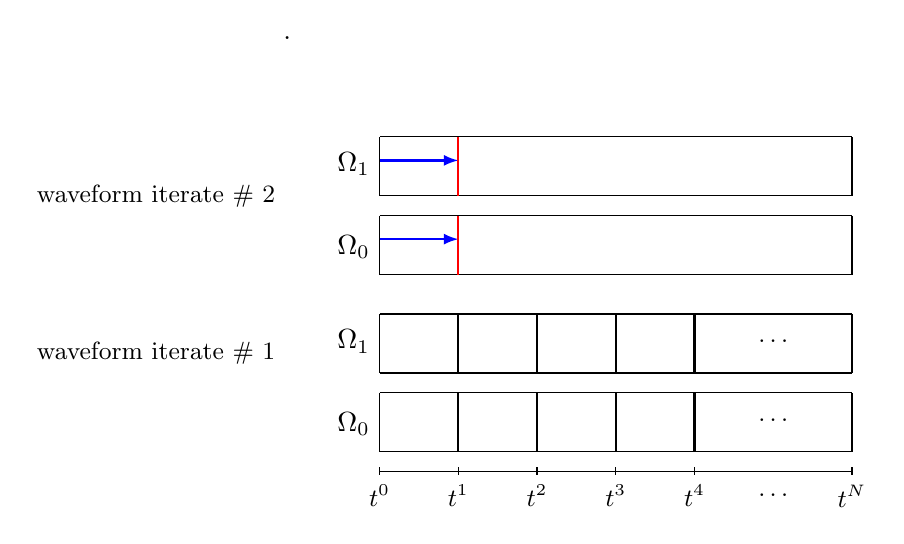
\begin{tikzpicture}[scale=1.0]

    \tikzstyle{dropline_style}=[densely dotted,thin]

    %\foreach \x/\xtext in {-1, -0.5/-\frac{1}{2}, 1}
    %\draw (\x cm,1pt) -- (\x cm,-1pt) node[anchor=north] {$\xtext$};

    \draw(-2,5) node[left] {.};
    \draw (-2.2, 1) node[left] {\small waveform iterate \# 1};
    \draw (-2.2, 3) node[left] {\small waveform iterate \# 2};
    %\draw (-2.2, 2) node[left] {\small waveform iterate \# 3};
    %\draw (-2.2, 3) node[left] {\small waveform iterate \# 4};
    %\draw (-2.2, 4) node[left] {\small waveform iterate \# 5};

    \def\a{-0.25}
    \def\b{0.5}
    \draw (-1,\a) -- (5,\a);
    \draw (5,\a) -- (5,\b);
    \draw (5,\b) -- (-1,\b);
    \draw (-1,\b) -- (-1,\a);

    \def\c{0.75}
    \def\d{1.5}
    \draw (-1,\c) -- (5,\c);
    \draw (5,\c) -- (5,\d);
    \draw (5,\d) -- (-1,\d);
    \draw (-1,\d) -- (-1,\c);

    \draw(-1,0.1) node[left] {$\Omega_0$};
    \draw(-1,1.15) node[left] {$\Omega_1$};

    \def\e{2}
    \def\f{2.75}
    \draw (-1,\e) -- (5,\e);
    \draw (5,\e) -- (5,\f);
    \draw (5,\f) -- (-1,\f);
    \draw (-1,\f) -- (-1,\e);

    \def\g{3}
    \def\h{3.75}
    \draw (-1,\g) -- (5,\g);
    \draw (5,\g) -- (5,\h);
    \draw (5,\h) -- (-1,\h);
    \draw (-1,\h) -- (-1,\g);

    \draw(-1,2.35) node[left] {$\Omega_0$};
    \draw(-1,3.4) node[left] {$\Omega_1$};

%\draw (2,0.2) -- (2,-0.2) node[below] {$\alpha$};
%\draw (4,0.2) -- (4,-0.2) node[below] {1};

    % position of the time-line
    \def\y{-0.5}
    \draw [-] (-1,\y) -- (5,\y);

    \def\tick{0.05}
    \draw (-1,\y) ++(0,\tick) -- ++(0,-2*\tick) node[below] {\small $t^{0}$};
    \draw (0,\y) ++(0,\tick) -- ++(0,-2*\tick) node[below] {\small $t^{1}$};
    \draw (1,\y) ++(0,\tick) -- ++(0,-2*\tick) node[below] {\small $t^{2}$};
    \draw (2,\y) ++(0,\tick) -- ++(0,-2*\tick) node[below] {\small $t^{3}$};
    \draw (3,\y) ++(0,\tick) -- ++(0,-2*\tick) node[below] {\small $t^{4}$};
    \draw (4,\y)  node[below] {\small \phantom{t}$\ldots$\phantom{t}};  
    \draw (5,\y) ++(0,\tick) -- ++(0,-2*\tick) node[below] {\small $t^{N}$};
  
    % parameters for stencil diagrams
    \def\rad{0.12}
    \def\omr{0.88}   % 1-rad
    \def\intthick{0.068}   % thickness of integral bars

    % filled dots
    %\foreach \xy in { (-1,0) }
    %\filldraw \xy circle (2pt);

    % hollow dots
    %\foreach \xy in { (0,0)}
    %\filldraw[fill=white] \xy circle (2.5pt);

    %\draw [-latex,thick,blue] (2,0.2) -- (3,0.2);
    %\draw [-latex,thick,blue] (2,1.2) -- (3,1.2);

    \draw [-,thick,black] (0,\a) -- (0,\b);
    \draw [-,thick,black] (0,\c) -- (0,\d);

    \draw [-,thick,black] (1,\a) -- (1,\b);
    \draw [-,thick,black] (1,\c) -- (1,\d);

    \draw [-,thick,black] (2,\a) -- (2,\b);
    \draw [-,thick,black] (2,\c) -- (2,\d);

    \draw [-,thick,black] (3,\a) -- (3,\b);
    \draw [-,thick,black] (3,\c) -- (3,\d);

    \draw (4,0.45)  node[below] {\small \phantom{t}$\ldots$\phantom{t}};  
    \draw (4,1.45)  node[below] {\small \phantom{t}$\ldots$\phantom{t}};  

    \draw [-latex,thick,blue] (-1,2.45) -- (0,2.45);
    \draw [-latex,thick,blue] (-1,3.45) -- (0,3.45);

    \draw [-,thick,red] (0,\e) -- (0,\f);
    \draw [-,thick,red] (0,\g) -- (0,\h);
    
  \end{tikzpicture}

    \end{figure}
  }
  \only<14>{
    \begin{figure}
      \centering
       \definecolor{darkgreen}{rgb}{0,.6,0}
  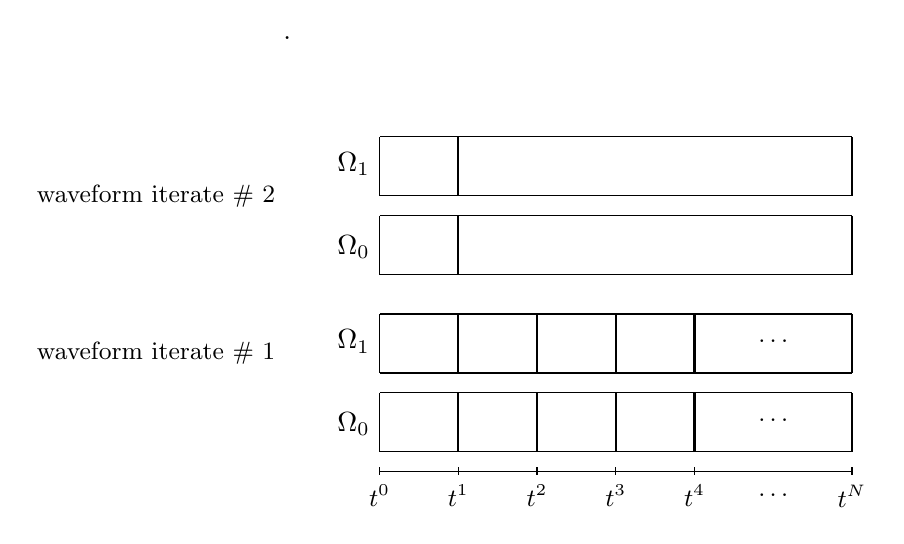
\begin{tikzpicture}[scale=1.0]

    \tikzstyle{dropline_style}=[densely dotted,thin]

    %\foreach \x/\xtext in {-1, -0.5/-\frac{1}{2}, 1}
    %\draw (\x cm,1pt) -- (\x cm,-1pt) node[anchor=north] {$\xtext$};

    \draw(-2,5) node[left] {.};
    \draw (-2.2, 1) node[left] {\small waveform iterate \# 1};
    \draw (-2.2, 3) node[left] {\small waveform iterate \# 2};
    %\draw (-2.2, 2) node[left] {\small waveform iterate \# 3};
    %\draw (-2.2, 3) node[left] {\small waveform iterate \# 4};
    %\draw (-2.2, 4) node[left] {\small waveform iterate \# 5};

    \def\a{-0.25}
    \def\b{0.5}
    \draw (-1,\a) -- (5,\a);
    \draw (5,\a) -- (5,\b);
    \draw (5,\b) -- (-1,\b);
    \draw (-1,\b) -- (-1,\a);

    \def\c{0.75}
    \def\d{1.5}
    \draw (-1,\c) -- (5,\c);
    \draw (5,\c) -- (5,\d);
    \draw (5,\d) -- (-1,\d);
    \draw (-1,\d) -- (-1,\c);

    \draw(-1,0.1) node[left] {$\Omega_0$};
    \draw(-1,1.15) node[left] {$\Omega_1$};

    \def\e{2}
    \def\f{2.75}
    \draw (-1,\e) -- (5,\e);
    \draw (5,\e) -- (5,\f);
    \draw (5,\f) -- (-1,\f);
    \draw (-1,\f) -- (-1,\e);

    \def\g{3}
    \def\h{3.75}
    \draw (-1,\g) -- (5,\g);
    \draw (5,\g) -- (5,\h);
    \draw (5,\h) -- (-1,\h);
    \draw (-1,\h) -- (-1,\g);

    \draw(-1,2.35) node[left] {$\Omega_0$};
    \draw(-1,3.4) node[left] {$\Omega_1$};

%\draw (2,0.2) -- (2,-0.2) node[below] {$\alpha$};
%\draw (4,0.2) -- (4,-0.2) node[below] {1};

    % position of the time-line
    \def\y{-0.5}
    \draw [-] (-1,\y) -- (5,\y);

    \def\tick{0.05}
    \draw (-1,\y) ++(0,\tick) -- ++(0,-2*\tick) node[below] {\small $t^{0}$};
    \draw (0,\y) ++(0,\tick) -- ++(0,-2*\tick) node[below] {\small $t^{1}$};
    \draw (1,\y) ++(0,\tick) -- ++(0,-2*\tick) node[below] {\small $t^{2}$};
    \draw (2,\y) ++(0,\tick) -- ++(0,-2*\tick) node[below] {\small $t^{3}$};
    \draw (3,\y) ++(0,\tick) -- ++(0,-2*\tick) node[below] {\small $t^{4}$};
    \draw (4,\y)  node[below] {\small \phantom{t}$\ldots$\phantom{t}};  
    \draw (5,\y) ++(0,\tick) -- ++(0,-2*\tick) node[below] {\small $t^{N}$};
  
    % parameters for stencil diagrams
    \def\rad{0.12}
    \def\omr{0.88}   % 1-rad
    \def\intthick{0.068}   % thickness of integral bars

    % filled dots
    %\foreach \xy in { (-1,0) }
    %\filldraw \xy circle (2pt);

    % hollow dots
    %\foreach \xy in { (0,0)}
    %\filldraw[fill=white] \xy circle (2.5pt);

    %\draw [-latex,thick,blue] (2,0.2) -- (3,0.2);
    %\draw [-latex,thick,blue] (2,1.2) -- (3,1.2);

    \draw [-,thick,black] (0,\a) -- (0,\b);
    \draw [-,thick,black] (0,\c) -- (0,\d);

    \draw [-,thick,black] (1,\a) -- (1,\b);
    \draw [-,thick,black] (1,\c) -- (1,\d);

    \draw [-,thick,black] (2,\a) -- (2,\b);
    \draw [-,thick,black] (2,\c) -- (2,\d);

    \draw [-,thick,black] (3,\a) -- (3,\b);
    \draw [-,thick,black] (3,\c) -- (3,\d);

    \draw (4,0.45)  node[below] {\small \phantom{t}$\ldots$\phantom{t}};  
    \draw (4,1.45)  node[below] {\small \phantom{t}$\ldots$\phantom{t}};  

    %\draw [-latex,thick,blue] (-1,2.45) -- (0,2.45);
    %\draw [-latex,thick,blue] (-1,3.45) -- (0,3.45);

    \draw [-,thick,black] (0,\e) -- (0,\f);
    \draw [-,thick,black] (0,\g) -- (0,\h);
    
  \end{tikzpicture}

    \end{figure}
  }
  \only<15>{
    \begin{figure}
      \centering
       \definecolor{darkgreen}{rgb}{0,.6,0}
  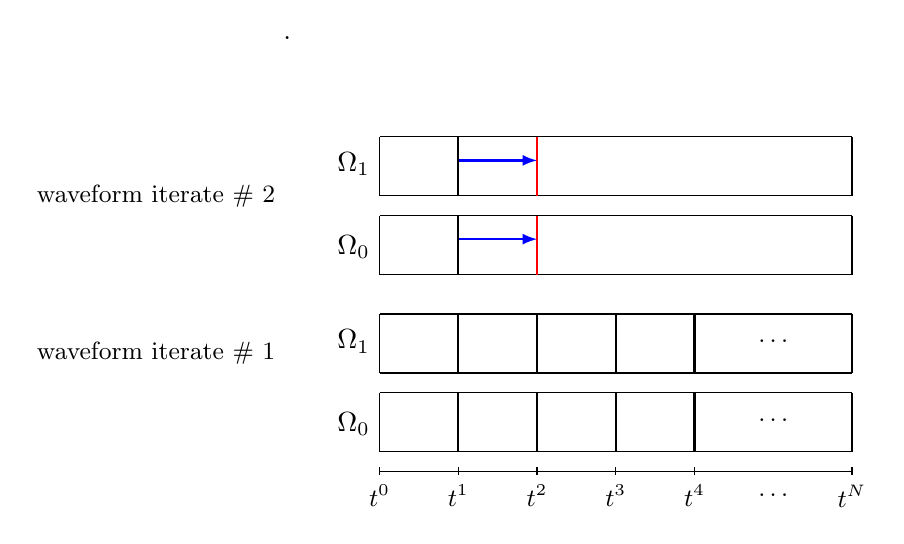
\begin{tikzpicture}[scale=1.0]

    \tikzstyle{dropline_style}=[densely dotted,thin]

    %\foreach \x/\xtext in {-1, -0.5/-\frac{1}{2}, 1}
    %\draw (\x cm,1pt) -- (\x cm,-1pt) node[anchor=north] {$\xtext$};

    \draw(-2,5) node[left] {.};
    \draw (-2.2, 1) node[left] {\small waveform iterate \# 1};
    \draw (-2.2, 3) node[left] {\small waveform iterate \# 2};
    %\draw (-2.2, 2) node[left] {\small waveform iterate \# 3};
    %\draw (-2.2, 3) node[left] {\small waveform iterate \# 4};
    %\draw (-2.2, 4) node[left] {\small waveform iterate \# 5};

    \def\a{-0.25}
    \def\b{0.5}
    \draw (-1,\a) -- (5,\a);
    \draw (5,\a) -- (5,\b);
    \draw (5,\b) -- (-1,\b);
    \draw (-1,\b) -- (-1,\a);

    \def\c{0.75}
    \def\d{1.5}
    \draw (-1,\c) -- (5,\c);
    \draw (5,\c) -- (5,\d);
    \draw (5,\d) -- (-1,\d);
    \draw (-1,\d) -- (-1,\c);

    \draw(-1,0.1) node[left] {$\Omega_0$};
    \draw(-1,1.15) node[left] {$\Omega_1$};

    \def\e{2}
    \def\f{2.75}
    \draw (-1,\e) -- (5,\e);
    \draw (5,\e) -- (5,\f);
    \draw (5,\f) -- (-1,\f);
    \draw (-1,\f) -- (-1,\e);

    \def\g{3}
    \def\h{3.75}
    \draw (-1,\g) -- (5,\g);
    \draw (5,\g) -- (5,\h);
    \draw (5,\h) -- (-1,\h);
    \draw (-1,\h) -- (-1,\g);

    \draw(-1,2.35) node[left] {$\Omega_0$};
    \draw(-1,3.4) node[left] {$\Omega_1$};

%\draw (2,0.2) -- (2,-0.2) node[below] {$\alpha$};
%\draw (4,0.2) -- (4,-0.2) node[below] {1};

    % position of the time-line
    \def\y{-0.5}
    \draw [-] (-1,\y) -- (5,\y);

    \def\tick{0.05}
    \draw (-1,\y) ++(0,\tick) -- ++(0,-2*\tick) node[below] {\small $t^{0}$};
    \draw (0,\y) ++(0,\tick) -- ++(0,-2*\tick) node[below] {\small $t^{1}$};
    \draw (1,\y) ++(0,\tick) -- ++(0,-2*\tick) node[below] {\small $t^{2}$};
    \draw (2,\y) ++(0,\tick) -- ++(0,-2*\tick) node[below] {\small $t^{3}$};
    \draw (3,\y) ++(0,\tick) -- ++(0,-2*\tick) node[below] {\small $t^{4}$};
    \draw (4,\y)  node[below] {\small \phantom{t}$\ldots$\phantom{t}};  
    \draw (5,\y) ++(0,\tick) -- ++(0,-2*\tick) node[below] {\small $t^{N}$};
  
    % parameters for stencil diagrams
    \def\rad{0.12}
    \def\omr{0.88}   % 1-rad
    \def\intthick{0.068}   % thickness of integral bars

    % filled dots
    %\foreach \xy in { (-1,0) }
    %\filldraw \xy circle (2pt);

    % hollow dots
    %\foreach \xy in { (0,0)}
    %\filldraw[fill=white] \xy circle (2.5pt);

    %\draw [-latex,thick,blue] (2,0.2) -- (3,0.2);
    %\draw [-latex,thick,blue] (2,1.2) -- (3,1.2);

    \draw [-,thick,black] (0,\a) -- (0,\b);
    \draw [-,thick,black] (0,\c) -- (0,\d);

    \draw [-,thick,black] (1,\a) -- (1,\b);
    \draw [-,thick,black] (1,\c) -- (1,\d);

    \draw [-,thick,black] (2,\a) -- (2,\b);
    \draw [-,thick,black] (2,\c) -- (2,\d);

    \draw [-,thick,black] (3,\a) -- (3,\b);
    \draw [-,thick,black] (3,\c) -- (3,\d);

    \draw (4,0.45)  node[below] {\small \phantom{t}$\ldots$\phantom{t}};  
    \draw (4,1.45)  node[below] {\small \phantom{t}$\ldots$\phantom{t}};  

    \draw [-latex,thick,blue] (0,2.45) -- (1,2.45);
    \draw [-latex,thick,blue] (0,3.45) -- (1,3.45);

    \draw [-,thick,black] (0,\e) -- (0,\f);
    \draw [-,thick,black] (0,\g) -- (0,\h);
    
    \draw [-,thick,red] (1,\e) -- (1,\f);
    \draw [-,thick,red] (1,\g) -- (1,\h);
    
  \end{tikzpicture}

    \end{figure}
  }
  \only<16>{
    \begin{figure}
      \centering
       \definecolor{darkgreen}{rgb}{0,.6,0}
  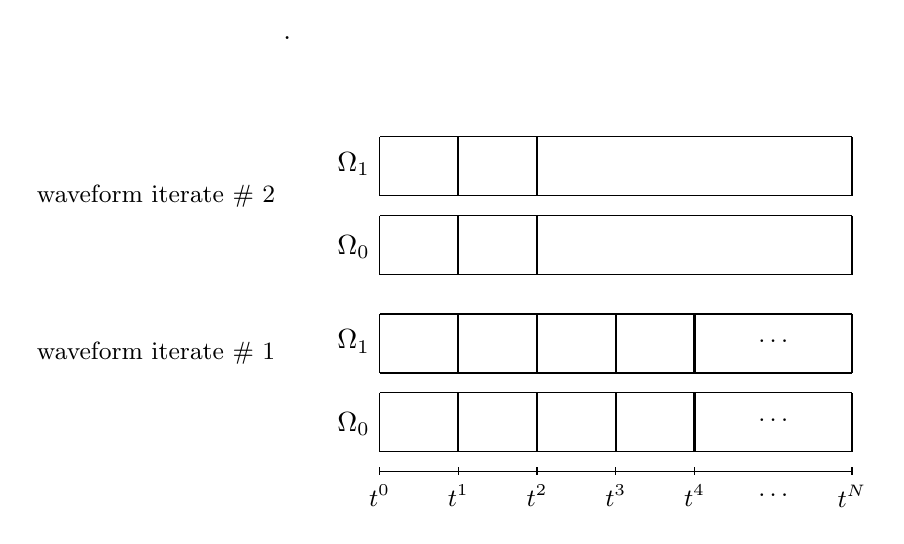
\begin{tikzpicture}[scale=1.0]

    \tikzstyle{dropline_style}=[densely dotted,thin]

    %\foreach \x/\xtext in {-1, -0.5/-\frac{1}{2}, 1}
    %\draw (\x cm,1pt) -- (\x cm,-1pt) node[anchor=north] {$\xtext$};

    \draw(-2,5) node[left] {.};
    \draw (-2.2, 1) node[left] {\small waveform iterate \# 1};
    \draw (-2.2, 3) node[left] {\small waveform iterate \# 2};
    %\draw (-2.2, 2) node[left] {\small waveform iterate \# 3};
    %\draw (-2.2, 3) node[left] {\small waveform iterate \# 4};
    %\draw (-2.2, 4) node[left] {\small waveform iterate \# 5};

    \def\a{-0.25}
    \def\b{0.5}
    \draw (-1,\a) -- (5,\a);
    \draw (5,\a) -- (5,\b);
    \draw (5,\b) -- (-1,\b);
    \draw (-1,\b) -- (-1,\a);

    \def\c{0.75}
    \def\d{1.5}
    \draw (-1,\c) -- (5,\c);
    \draw (5,\c) -- (5,\d);
    \draw (5,\d) -- (-1,\d);
    \draw (-1,\d) -- (-1,\c);

    \draw(-1,0.1) node[left] {$\Omega_0$};
    \draw(-1,1.15) node[left] {$\Omega_1$};

    \def\e{2}
    \def\f{2.75}
    \draw (-1,\e) -- (5,\e);
    \draw (5,\e) -- (5,\f);
    \draw (5,\f) -- (-1,\f);
    \draw (-1,\f) -- (-1,\e);

    \def\g{3}
    \def\h{3.75}
    \draw (-1,\g) -- (5,\g);
    \draw (5,\g) -- (5,\h);
    \draw (5,\h) -- (-1,\h);
    \draw (-1,\h) -- (-1,\g);

    \draw(-1,2.35) node[left] {$\Omega_0$};
    \draw(-1,3.4) node[left] {$\Omega_1$};

%\draw (2,0.2) -- (2,-0.2) node[below] {$\alpha$};
%\draw (4,0.2) -- (4,-0.2) node[below] {1};

    % position of the time-line
    \def\y{-0.5}
    \draw [-] (-1,\y) -- (5,\y);

    \def\tick{0.05}
    \draw (-1,\y) ++(0,\tick) -- ++(0,-2*\tick) node[below] {\small $t^{0}$};
    \draw (0,\y) ++(0,\tick) -- ++(0,-2*\tick) node[below] {\small $t^{1}$};
    \draw (1,\y) ++(0,\tick) -- ++(0,-2*\tick) node[below] {\small $t^{2}$};
    \draw (2,\y) ++(0,\tick) -- ++(0,-2*\tick) node[below] {\small $t^{3}$};
    \draw (3,\y) ++(0,\tick) -- ++(0,-2*\tick) node[below] {\small $t^{4}$};
    \draw (4,\y)  node[below] {\small \phantom{t}$\ldots$\phantom{t}};  
    \draw (5,\y) ++(0,\tick) -- ++(0,-2*\tick) node[below] {\small $t^{N}$};
  
    % parameters for stencil diagrams
    \def\rad{0.12}
    \def\omr{0.88}   % 1-rad
    \def\intthick{0.068}   % thickness of integral bars

    % filled dots
    %\foreach \xy in { (-1,0) }
    %\filldraw \xy circle (2pt);

    % hollow dots
    %\foreach \xy in { (0,0)}
    %\filldraw[fill=white] \xy circle (2.5pt);

    %\draw [-latex,thick,blue] (2,0.2) -- (3,0.2);
    %\draw [-latex,thick,blue] (2,1.2) -- (3,1.2);

    \draw [-,thick,black] (0,\a) -- (0,\b);
    \draw [-,thick,black] (0,\c) -- (0,\d);

    \draw [-,thick,black] (1,\a) -- (1,\b);
    \draw [-,thick,black] (1,\c) -- (1,\d);

    \draw [-,thick,black] (2,\a) -- (2,\b);
    \draw [-,thick,black] (2,\c) -- (2,\d);

    \draw [-,thick,black] (3,\a) -- (3,\b);
    \draw [-,thick,black] (3,\c) -- (3,\d);

    \draw (4,0.45)  node[below] {\small \phantom{t}$\ldots$\phantom{t}};  
    \draw (4,1.45)  node[below] {\small \phantom{t}$\ldots$\phantom{t}};  

    %\draw [-latex,thick,blue] (0,2.45) -- (1,2.45);
    %\draw [-latex,thick,blue] (0,3.45) -- (1,3.45);

    \draw [-,thick,black] (0,\e) -- (0,\f);
    \draw [-,thick,black] (0,\g) -- (0,\h);
    
    \draw [-,thick,black] (1,\e) -- (1,\f);
    \draw [-,thick,black] (1,\g) -- (1,\h);
    
  \end{tikzpicture}

    \end{figure}
  }
  \only<17>{
    \begin{figure}
      \centering
       \definecolor{darkgreen}{rgb}{0,.6,0}
  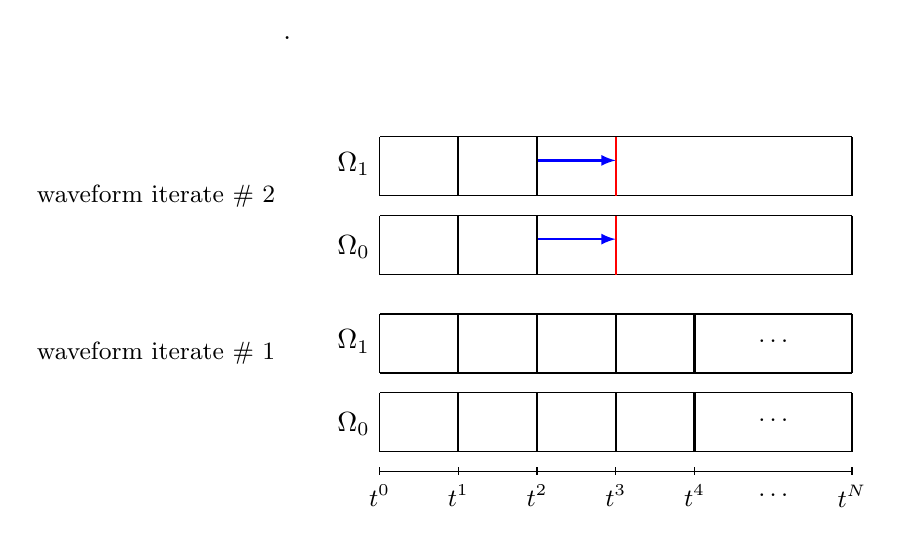
\begin{tikzpicture}[scale=1.0]

    \tikzstyle{dropline_style}=[densely dotted,thin]

    %\foreach \x/\xtext in {-1, -0.5/-\frac{1}{2}, 1}
    %\draw (\x cm,1pt) -- (\x cm,-1pt) node[anchor=north] {$\xtext$};

    \draw(-2,5) node[left] {.};
    \draw (-2.2, 1) node[left] {\small waveform iterate \# 1};
    \draw (-2.2, 3) node[left] {\small waveform iterate \# 2};
    %\draw (-2.2, 2) node[left] {\small waveform iterate \# 3};
    %\draw (-2.2, 3) node[left] {\small waveform iterate \# 4};
    %\draw (-2.2, 4) node[left] {\small waveform iterate \# 5};

    \def\a{-0.25}
    \def\b{0.5}
    \draw (-1,\a) -- (5,\a);
    \draw (5,\a) -- (5,\b);
    \draw (5,\b) -- (-1,\b);
    \draw (-1,\b) -- (-1,\a);

    \def\c{0.75}
    \def\d{1.5}
    \draw (-1,\c) -- (5,\c);
    \draw (5,\c) -- (5,\d);
    \draw (5,\d) -- (-1,\d);
    \draw (-1,\d) -- (-1,\c);

    \draw(-1,0.1) node[left] {$\Omega_0$};
    \draw(-1,1.15) node[left] {$\Omega_1$};

    \def\e{2}
    \def\f{2.75}
    \draw (-1,\e) -- (5,\e);
    \draw (5,\e) -- (5,\f);
    \draw (5,\f) -- (-1,\f);
    \draw (-1,\f) -- (-1,\e);

    \def\g{3}
    \def\h{3.75}
    \draw (-1,\g) -- (5,\g);
    \draw (5,\g) -- (5,\h);
    \draw (5,\h) -- (-1,\h);
    \draw (-1,\h) -- (-1,\g);

    \draw(-1,2.35) node[left] {$\Omega_0$};
    \draw(-1,3.4) node[left] {$\Omega_1$};

%\draw (2,0.2) -- (2,-0.2) node[below] {$\alpha$};
%\draw (4,0.2) -- (4,-0.2) node[below] {1};

    % position of the time-line
    \def\y{-0.5}
    \draw [-] (-1,\y) -- (5,\y);

    \def\tick{0.05}
    \draw (-1,\y) ++(0,\tick) -- ++(0,-2*\tick) node[below] {\small $t^{0}$};
    \draw (0,\y) ++(0,\tick) -- ++(0,-2*\tick) node[below] {\small $t^{1}$};
    \draw (1,\y) ++(0,\tick) -- ++(0,-2*\tick) node[below] {\small $t^{2}$};
    \draw (2,\y) ++(0,\tick) -- ++(0,-2*\tick) node[below] {\small $t^{3}$};
    \draw (3,\y) ++(0,\tick) -- ++(0,-2*\tick) node[below] {\small $t^{4}$};
    \draw (4,\y)  node[below] {\small \phantom{t}$\ldots$\phantom{t}};  
    \draw (5,\y) ++(0,\tick) -- ++(0,-2*\tick) node[below] {\small $t^{N}$};
  
    % parameters for stencil diagrams
    \def\rad{0.12}
    \def\omr{0.88}   % 1-rad
    \def\intthick{0.068}   % thickness of integral bars

    % filled dots
    %\foreach \xy in { (-1,0) }
    %\filldraw \xy circle (2pt);

    % hollow dots
    %\foreach \xy in { (0,0)}
    %\filldraw[fill=white] \xy circle (2.5pt);

    %\draw [-latex,thick,blue] (2,0.2) -- (3,0.2);
    %\draw [-latex,thick,blue] (2,1.2) -- (3,1.2);

    \draw [-,thick,black] (0,\a) -- (0,\b);
    \draw [-,thick,black] (0,\c) -- (0,\d);

    \draw [-,thick,black] (1,\a) -- (1,\b);
    \draw [-,thick,black] (1,\c) -- (1,\d);

    \draw [-,thick,black] (2,\a) -- (2,\b);
    \draw [-,thick,black] (2,\c) -- (2,\d);

    \draw [-,thick,black] (3,\a) -- (3,\b);
    \draw [-,thick,black] (3,\c) -- (3,\d);

    \draw (4,0.45)  node[below] {\small \phantom{t}$\ldots$\phantom{t}};  
    \draw (4,1.45)  node[below] {\small \phantom{t}$\ldots$\phantom{t}};  

    \draw [-latex,thick,blue] (1,2.45) -- (2,2.45);
    \draw [-latex,thick,blue] (1,3.45) -- (2,3.45);

    \draw [-,thick,black] (0,\e) -- (0,\f);
    \draw [-,thick,black] (0,\g) -- (0,\h);
    
    \draw [-,thick,black] (1,\e) -- (1,\f);
    \draw [-,thick,black] (1,\g) -- (1,\h);

    \draw [-,thick,red] (2,\e) -- (2,\f);
    \draw [-,thick,red] (2,\g) -- (2,\h);
    
  \end{tikzpicture}

    \end{figure}
  }
  \only<18>{
    \begin{figure}
      \centering
       \definecolor{darkgreen}{rgb}{0,.6,0}
  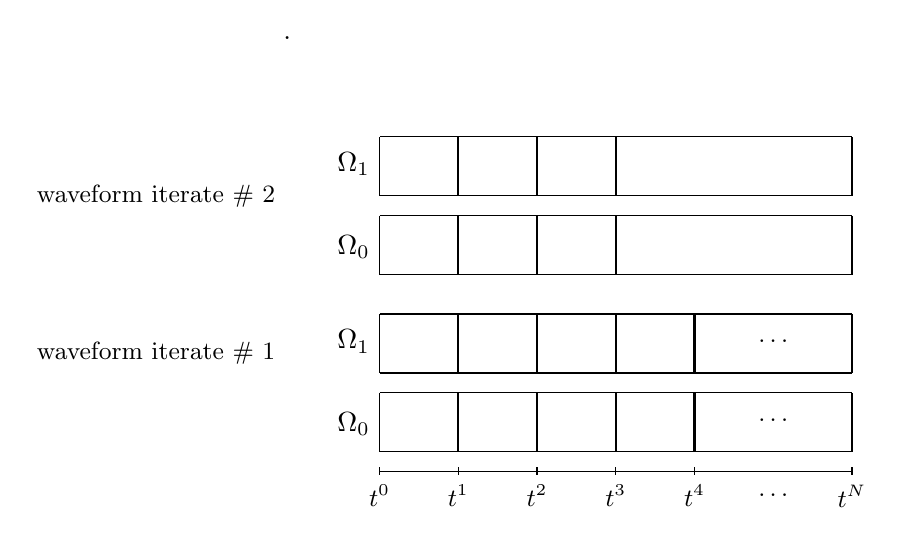
\begin{tikzpicture}[scale=1.0]

    \tikzstyle{dropline_style}=[densely dotted,thin]

    %\foreach \x/\xtext in {-1, -0.5/-\frac{1}{2}, 1}
    %\draw (\x cm,1pt) -- (\x cm,-1pt) node[anchor=north] {$\xtext$};

    \draw(-2,5) node[left] {.};
    \draw (-2.2, 1) node[left] {\small waveform iterate \# 1};
    \draw (-2.2, 3) node[left] {\small waveform iterate \# 2};
    %\draw (-2.2, 2) node[left] {\small waveform iterate \# 3};
    %\draw (-2.2, 3) node[left] {\small waveform iterate \# 4};
    %\draw (-2.2, 4) node[left] {\small waveform iterate \# 5};

    \def\a{-0.25}
    \def\b{0.5}
    \draw (-1,\a) -- (5,\a);
    \draw (5,\a) -- (5,\b);
    \draw (5,\b) -- (-1,\b);
    \draw (-1,\b) -- (-1,\a);

    \def\c{0.75}
    \def\d{1.5}
    \draw (-1,\c) -- (5,\c);
    \draw (5,\c) -- (5,\d);
    \draw (5,\d) -- (-1,\d);
    \draw (-1,\d) -- (-1,\c);

    \draw(-1,0.1) node[left] {$\Omega_0$};
    \draw(-1,1.15) node[left] {$\Omega_1$};

    \def\e{2}
    \def\f{2.75}
    \draw (-1,\e) -- (5,\e);
    \draw (5,\e) -- (5,\f);
    \draw (5,\f) -- (-1,\f);
    \draw (-1,\f) -- (-1,\e);

    \def\g{3}
    \def\h{3.75}
    \draw (-1,\g) -- (5,\g);
    \draw (5,\g) -- (5,\h);
    \draw (5,\h) -- (-1,\h);
    \draw (-1,\h) -- (-1,\g);

    \draw(-1,2.35) node[left] {$\Omega_0$};
    \draw(-1,3.4) node[left] {$\Omega_1$};

%\draw (2,0.2) -- (2,-0.2) node[below] {$\alpha$};
%\draw (4,0.2) -- (4,-0.2) node[below] {1};

    % position of the time-line
    \def\y{-0.5}
    \draw [-] (-1,\y) -- (5,\y);

    \def\tick{0.05}
    \draw (-1,\y) ++(0,\tick) -- ++(0,-2*\tick) node[below] {\small $t^{0}$};
    \draw (0,\y) ++(0,\tick) -- ++(0,-2*\tick) node[below] {\small $t^{1}$};
    \draw (1,\y) ++(0,\tick) -- ++(0,-2*\tick) node[below] {\small $t^{2}$};
    \draw (2,\y) ++(0,\tick) -- ++(0,-2*\tick) node[below] {\small $t^{3}$};
    \draw (3,\y) ++(0,\tick) -- ++(0,-2*\tick) node[below] {\small $t^{4}$};
    \draw (4,\y)  node[below] {\small \phantom{t}$\ldots$\phantom{t}};  
    \draw (5,\y) ++(0,\tick) -- ++(0,-2*\tick) node[below] {\small $t^{N}$};
  
    % parameters for stencil diagrams
    \def\rad{0.12}
    \def\omr{0.88}   % 1-rad
    \def\intthick{0.068}   % thickness of integral bars

    % filled dots
    %\foreach \xy in { (-1,0) }
    %\filldraw \xy circle (2pt);

    % hollow dots
    %\foreach \xy in { (0,0)}
    %\filldraw[fill=white] \xy circle (2.5pt);

    %\draw [-latex,thick,blue] (2,0.2) -- (3,0.2);
    %\draw [-latex,thick,blue] (2,1.2) -- (3,1.2);

    \draw [-,thick,black] (0,\a) -- (0,\b);
    \draw [-,thick,black] (0,\c) -- (0,\d);

    \draw [-,thick,black] (1,\a) -- (1,\b);
    \draw [-,thick,black] (1,\c) -- (1,\d);

    \draw [-,thick,black] (2,\a) -- (2,\b);
    \draw [-,thick,black] (2,\c) -- (2,\d);

    \draw [-,thick,black] (3,\a) -- (3,\b);
    \draw [-,thick,black] (3,\c) -- (3,\d);

    \draw (4,0.45)  node[below] {\small \phantom{t}$\ldots$\phantom{t}};  
    \draw (4,1.45)  node[below] {\small \phantom{t}$\ldots$\phantom{t}};  

    %\draw [-latex,thick,blue] (1,2.45) -- (2,2.45);
    %\draw [-latex,thick,blue] (1,3.45) -- (2,3.45);

    \draw [-,thick,black] (0,\e) -- (0,\f);
    \draw [-,thick,black] (0,\g) -- (0,\h);
    
    \draw [-,thick,black] (1,\e) -- (1,\f);
    \draw [-,thick,black] (1,\g) -- (1,\h);

    \draw [-,thick,black] (2,\e) -- (2,\f);
    \draw [-,thick,black] (2,\g) -- (2,\h);
    
  \end{tikzpicture}

    \end{figure}
  }
  \only<19>{
    \begin{figure}
      \centering
       \definecolor{darkgreen}{rgb}{0,.6,0}
  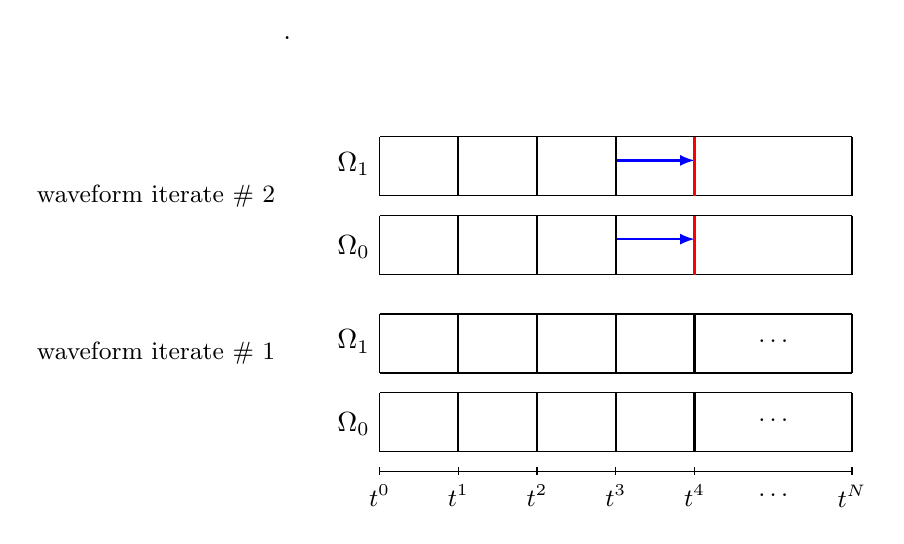
\begin{tikzpicture}[scale=1.0]

    \tikzstyle{dropline_style}=[densely dotted,thin]

    %\foreach \x/\xtext in {-1, -0.5/-\frac{1}{2}, 1}
    %\draw (\x cm,1pt) -- (\x cm,-1pt) node[anchor=north] {$\xtext$};

    \draw(-2,5) node[left] {.};
    \draw (-2.2, 1) node[left] {\small waveform iterate \# 1};
    \draw (-2.2, 3) node[left] {\small waveform iterate \# 2};
    %\draw (-2.2, 2) node[left] {\small waveform iterate \# 3};
    %\draw (-2.2, 3) node[left] {\small waveform iterate \# 4};
    %\draw (-2.2, 4) node[left] {\small waveform iterate \# 5};

    \def\a{-0.25}
    \def\b{0.5}
    \draw (-1,\a) -- (5,\a);
    \draw (5,\a) -- (5,\b);
    \draw (5,\b) -- (-1,\b);
    \draw (-1,\b) -- (-1,\a);

    \def\c{0.75}
    \def\d{1.5}
    \draw (-1,\c) -- (5,\c);
    \draw (5,\c) -- (5,\d);
    \draw (5,\d) -- (-1,\d);
    \draw (-1,\d) -- (-1,\c);

    \draw(-1,0.1) node[left] {$\Omega_0$};
    \draw(-1,1.15) node[left] {$\Omega_1$};

    \def\e{2}
    \def\f{2.75}
    \draw (-1,\e) -- (5,\e);
    \draw (5,\e) -- (5,\f);
    \draw (5,\f) -- (-1,\f);
    \draw (-1,\f) -- (-1,\e);

    \def\g{3}
    \def\h{3.75}
    \draw (-1,\g) -- (5,\g);
    \draw (5,\g) -- (5,\h);
    \draw (5,\h) -- (-1,\h);
    \draw (-1,\h) -- (-1,\g);

    \draw(-1,2.35) node[left] {$\Omega_0$};
    \draw(-1,3.4) node[left] {$\Omega_1$};

%\draw (2,0.2) -- (2,-0.2) node[below] {$\alpha$};
%\draw (4,0.2) -- (4,-0.2) node[below] {1};

    % position of the time-line
    \def\y{-0.5}
    \draw [-] (-1,\y) -- (5,\y);

    \def\tick{0.05}
    \draw (-1,\y) ++(0,\tick) -- ++(0,-2*\tick) node[below] {\small $t^{0}$};
    \draw (0,\y) ++(0,\tick) -- ++(0,-2*\tick) node[below] {\small $t^{1}$};
    \draw (1,\y) ++(0,\tick) -- ++(0,-2*\tick) node[below] {\small $t^{2}$};
    \draw (2,\y) ++(0,\tick) -- ++(0,-2*\tick) node[below] {\small $t^{3}$};
    \draw (3,\y) ++(0,\tick) -- ++(0,-2*\tick) node[below] {\small $t^{4}$};
    \draw (4,\y)  node[below] {\small \phantom{t}$\ldots$\phantom{t}};  
    \draw (5,\y) ++(0,\tick) -- ++(0,-2*\tick) node[below] {\small $t^{N}$};
  
    % parameters for stencil diagrams
    \def\rad{0.12}
    \def\omr{0.88}   % 1-rad
    \def\intthick{0.068}   % thickness of integral bars

    % filled dots
    %\foreach \xy in { (-1,0) }
    %\filldraw \xy circle (2pt);

    % hollow dots
    %\foreach \xy in { (0,0)}
    %\filldraw[fill=white] \xy circle (2.5pt);

    %\draw [-latex,thick,blue] (2,0.2) -- (3,0.2);
    %\draw [-latex,thick,blue] (2,1.2) -- (3,1.2);

    \draw [-,thick,black] (0,\a) -- (0,\b);
    \draw [-,thick,black] (0,\c) -- (0,\d);

    \draw [-,thick,black] (1,\a) -- (1,\b);
    \draw [-,thick,black] (1,\c) -- (1,\d);

    \draw [-,thick,black] (2,\a) -- (2,\b);
    \draw [-,thick,black] (2,\c) -- (2,\d);

    \draw [-,thick,black] (3,\a) -- (3,\b);
    \draw [-,thick,black] (3,\c) -- (3,\d);

    \draw (4,0.45)  node[below] {\small \phantom{t}$\ldots$\phantom{t}};  
    \draw (4,1.45)  node[below] {\small \phantom{t}$\ldots$\phantom{t}};  

    \draw [-latex,thick,blue] (2,2.45) -- (3,2.45);
    \draw [-latex,thick,blue] (2,3.45) -- (3,3.45);

    \draw [-,thick,black] (0,\e) -- (0,\f);
    \draw [-,thick,black] (0,\g) -- (0,\h);
    
    \draw [-,thick,black] (1,\e) -- (1,\f);
    \draw [-,thick,black] (1,\g) -- (1,\h);

    \draw [-,thick,black] (2,\e) -- (2,\f);
    \draw [-,thick,black] (2,\g) -- (2,\h);

    \draw [-,thick,red] (3,\e) -- (3,\f);
    \draw [-,thick,red] (3,\g) -- (3,\h);
    
  \end{tikzpicture}

    \end{figure}
  }
  \only<20>{
    \begin{figure}
      \centering
       \definecolor{darkgreen}{rgb}{0,.6,0}
  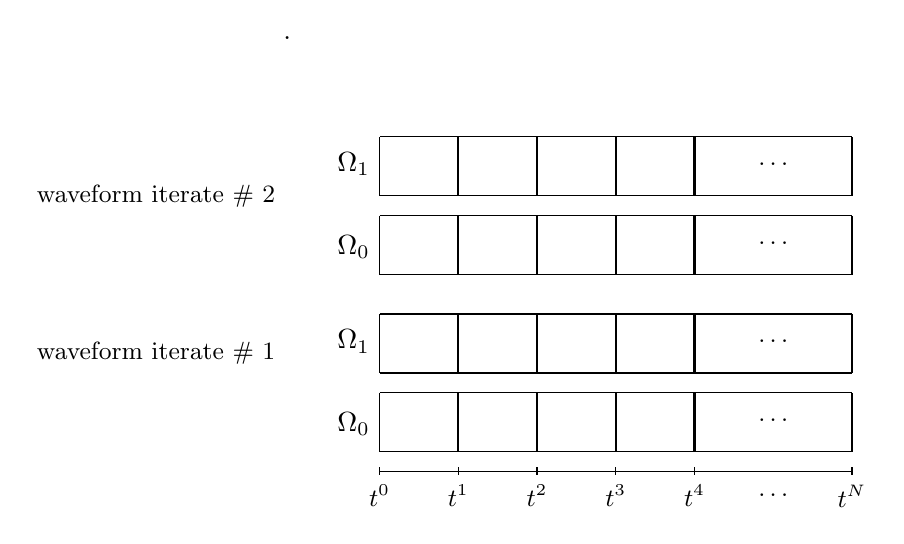
\begin{tikzpicture}[scale=1.0]

    \tikzstyle{dropline_style}=[densely dotted,thin]

    %\foreach \x/\xtext in {-1, -0.5/-\frac{1}{2}, 1}
    %\draw (\x cm,1pt) -- (\x cm,-1pt) node[anchor=north] {$\xtext$};

    \draw(-2,5) node[left] {.};
    \draw (-2.2, 1) node[left] {\small waveform iterate \# 1};
    \draw (-2.2, 3) node[left] {\small waveform iterate \# 2};
    %\draw (-2.2, 2) node[left] {\small waveform iterate \# 3};
    %\draw (-2.2, 3) node[left] {\small waveform iterate \# 4};
    %\draw (-2.2, 4) node[left] {\small waveform iterate \# 5};

    \def\a{-0.25}
    \def\b{0.5}
    \draw (-1,\a) -- (5,\a);
    \draw (5,\a) -- (5,\b);
    \draw (5,\b) -- (-1,\b);
    \draw (-1,\b) -- (-1,\a);

    \def\c{0.75}
    \def\d{1.5}
    \draw (-1,\c) -- (5,\c);
    \draw (5,\c) -- (5,\d);
    \draw (5,\d) -- (-1,\d);
    \draw (-1,\d) -- (-1,\c);

    \draw(-1,0.1) node[left] {$\Omega_0$};
    \draw(-1,1.15) node[left] {$\Omega_1$};

    \def\e{2}
    \def\f{2.75}
    \draw (-1,\e) -- (5,\e);
    \draw (5,\e) -- (5,\f);
    \draw (5,\f) -- (-1,\f);
    \draw (-1,\f) -- (-1,\e);

    \def\g{3}
    \def\h{3.75}
    \draw (-1,\g) -- (5,\g);
    \draw (5,\g) -- (5,\h);
    \draw (5,\h) -- (-1,\h);
    \draw (-1,\h) -- (-1,\g);

    \draw(-1,2.35) node[left] {$\Omega_0$};
    \draw(-1,3.4) node[left] {$\Omega_1$};

%\draw (2,0.2) -- (2,-0.2) node[below] {$\alpha$};
%\draw (4,0.2) -- (4,-0.2) node[below] {1};

    % position of the time-line
    \def\y{-0.5}
    \draw [-] (-1,\y) -- (5,\y);

    \def\tick{0.05}
    \draw (-1,\y) ++(0,\tick) -- ++(0,-2*\tick) node[below] {\small $t^{0}$};
    \draw (0,\y) ++(0,\tick) -- ++(0,-2*\tick) node[below] {\small $t^{1}$};
    \draw (1,\y) ++(0,\tick) -- ++(0,-2*\tick) node[below] {\small $t^{2}$};
    \draw (2,\y) ++(0,\tick) -- ++(0,-2*\tick) node[below] {\small $t^{3}$};
    \draw (3,\y) ++(0,\tick) -- ++(0,-2*\tick) node[below] {\small $t^{4}$};
    \draw (4,\y)  node[below] {\small \phantom{t}$\ldots$\phantom{t}};  
    \draw (5,\y) ++(0,\tick) -- ++(0,-2*\tick) node[below] {\small $t^{N}$};
  
    % parameters for stencil diagrams
    \def\rad{0.12}
    \def\omr{0.88}   % 1-rad
    \def\intthick{0.068}   % thickness of integral bars

    % filled dots
    %\foreach \xy in { (-1,0) }
    %\filldraw \xy circle (2pt);

    % hollow dots
    %\foreach \xy in { (0,0)}
    %\filldraw[fill=white] \xy circle (2.5pt);

    %\draw [-latex,thick,blue] (2,0.2) -- (3,0.2);
    %\draw [-latex,thick,blue] (2,1.2) -- (3,1.2);

    \draw [-,thick,black] (0,\a) -- (0,\b);
    \draw [-,thick,black] (0,\c) -- (0,\d);

    \draw [-,thick,black] (1,\a) -- (1,\b);
    \draw [-,thick,black] (1,\c) -- (1,\d);

    \draw [-,thick,black] (2,\a) -- (2,\b);
    \draw [-,thick,black] (2,\c) -- (2,\d);

    \draw [-,thick,black] (3,\a) -- (3,\b);
    \draw [-,thick,black] (3,\c) -- (3,\d);

    \draw (4,0.45)  node[below] {\small \phantom{t}$\ldots$\phantom{t}};  
    \draw (4,1.45)  node[below] {\small \phantom{t}$\ldots$\phantom{t}};  

    %\draw [-latex,thick,blue] (2,2.45) -- (3,2.45);
    %\draw [-latex,thick,blue] (2,3.45) -- (3,3.45);

    \draw [-,thick,black] (0,\e) -- (0,\f);
    \draw [-,thick,black] (0,\g) -- (0,\h);
    
    \draw [-,thick,black] (1,\e) -- (1,\f);
    \draw [-,thick,black] (1,\g) -- (1,\h);

    \draw [-,thick,black] (2,\e) -- (2,\f);
    \draw [-,thick,black] (2,\g) -- (2,\h);

    \draw [-,thick,black] (3,\e) -- (3,\f);
    \draw [-,thick,black] (3,\g) -- (3,\h);

    \draw (4,2.7)  node[below] {\small \phantom{t}$\ldots$\phantom{t}};  
    \draw (4,3.7)  node[below] {\small \phantom{t}$\ldots$\phantom{t}};  
    

  \end{tikzpicture}

    \end{figure}
  }
  \only<21>{
    \begin{figure}
      \centering
       \definecolor{darkgreen}{rgb}{0,.6,0}
  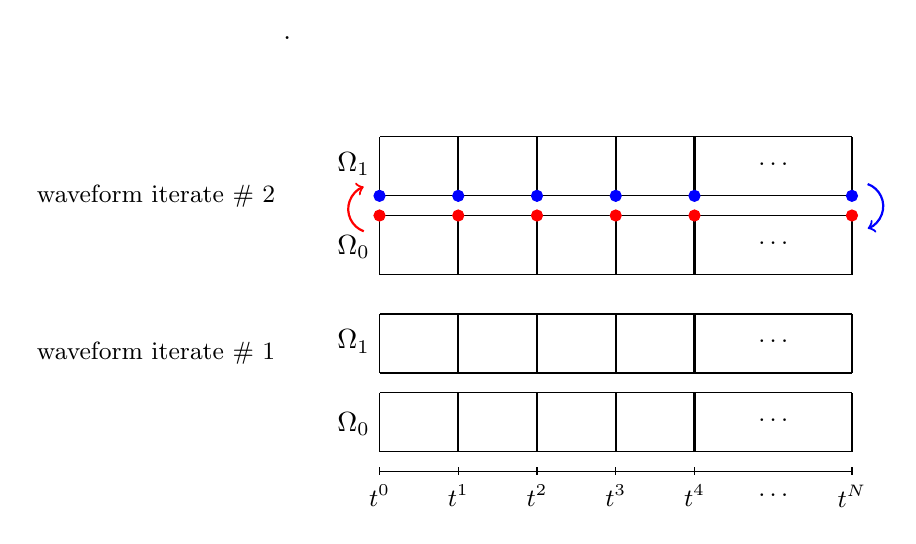
\begin{tikzpicture}[scale=1.0]

    \tikzstyle{dropline_style}=[densely dotted,thin]

    %\foreach \x/\xtext in {-1, -0.5/-\frac{1}{2}, 1}
    %\draw (\x cm,1pt) -- (\x cm,-1pt) node[anchor=north] {$\xtext$};

    \draw(-2,5) node[left] {.};
    \draw (-2.2, 1) node[left] {\small waveform iterate \# 1};
    \draw (-2.2, 3) node[left] {\small waveform iterate \# 2};
    %\draw (-2.2, 2) node[left] {\small waveform iterate \# 3};
    %\draw (-2.2, 3) node[left] {\small waveform iterate \# 4};
    %\draw (-2.2, 4) node[left] {\small waveform iterate \# 5};

    \def\a{-0.25}
    \def\b{0.5}
    \draw (-1,\a) -- (5,\a);
    \draw (5,\a) -- (5,\b);
    \draw (5,\b) -- (-1,\b);
    \draw (-1,\b) -- (-1,\a);

    \def\c{0.75}
    \def\d{1.5}
    \draw (-1,\c) -- (5,\c);
    \draw (5,\c) -- (5,\d);
    \draw (5,\d) -- (-1,\d);
    \draw (-1,\d) -- (-1,\c);

    \draw(-1,0.1) node[left] {$\Omega_0$};
    \draw(-1,1.15) node[left] {$\Omega_1$};

    \def\e{2}
    \def\f{2.75}
    \draw (-1,\e) -- (5,\e);
    \draw (5,\e) -- (5,\f);
    \draw (5,\f) -- (-1,\f);
    \draw (-1,\f) -- (-1,\e);

    \def\g{3}
    \def\h{3.75}
    \draw (-1,\g) -- (5,\g);
    \draw (5,\g) -- (5,\h);
    \draw (5,\h) -- (-1,\h);
    \draw (-1,\h) -- (-1,\g);

    \draw(-1,2.35) node[left] {$\Omega_0$};
    \draw(-1,3.4) node[left] {$\Omega_1$};

%\draw (2,0.2) -- (2,-0.2) node[below] {$\alpha$};
%\draw (4,0.2) -- (4,-0.2) node[below] {1};

    % position of the time-line
    \def\y{-0.5}
    \draw [-] (-1,\y) -- (5,\y);

    \def\tick{0.05}
    \draw (-1,\y) ++(0,\tick) -- ++(0,-2*\tick) node[below] {\small $t^{0}$};
    \draw (0,\y) ++(0,\tick) -- ++(0,-2*\tick) node[below] {\small $t^{1}$};
    \draw (1,\y) ++(0,\tick) -- ++(0,-2*\tick) node[below] {\small $t^{2}$};
    \draw (2,\y) ++(0,\tick) -- ++(0,-2*\tick) node[below] {\small $t^{3}$};
    \draw (3,\y) ++(0,\tick) -- ++(0,-2*\tick) node[below] {\small $t^{4}$};
    \draw (4,\y)  node[below] {\small \phantom{t}$\ldots$\phantom{t}};  
    \draw (5,\y) ++(0,\tick) -- ++(0,-2*\tick) node[below] {\small $t^{N}$};
  
    % parameters for stencil diagrams
    \def\rad{0.12}
    \def\omr{0.88}   % 1-rad
    \def\intthick{0.068}   % thickness of integral bars

    % filled dots
    %\foreach \xy in { (-1,0) }
    %\filldraw \xy circle (2pt);

    % hollow dots
    %\foreach \xy in { (0,0)}
    %\filldraw[fill=white] \xy circle (2.5pt);

    %\draw [-latex,thick,blue] (2,0.2) -- (3,0.2);
    %\draw [-latex,thick,blue] (2,1.2) -- (3,1.2);

    \draw [-,thick,black] (0,\a) -- (0,\b);
    \draw [-,thick,black] (0,\c) -- (0,\d);

    \draw [-,thick,black] (1,\a) -- (1,\b);
    \draw [-,thick,black] (1,\c) -- (1,\d);

    \draw [-,thick,black] (2,\a) -- (2,\b);
    \draw [-,thick,black] (2,\c) -- (2,\d);

    \draw [-,thick,black] (3,\a) -- (3,\b);
    \draw [-,thick,black] (3,\c) -- (3,\d);

    \draw (4,0.45)  node[below] {\small \phantom{t}$\ldots$\phantom{t}};  
    \draw (4,1.45)  node[below] {\small \phantom{t}$\ldots$\phantom{t}};  

    %\draw [-latex,thick,blue] (2,2.45) -- (3,2.45);
    %\draw [-latex,thick,blue] (2,3.45) -- (3,3.45);

    \draw [-,thick,black] (0,\e) -- (0,\f);
    \draw [-,thick,black] (0,\g) -- (0,\h);
    
    \draw [-,thick,black] (1,\e) -- (1,\f);
    \draw [-,thick,black] (1,\g) -- (1,\h);

    \draw [-,thick,black] (2,\e) -- (2,\f);
    \draw [-,thick,black] (2,\g) -- (2,\h);

    \draw [-,thick,black] (3,\e) -- (3,\f);
    \draw [-,thick,black] (3,\g) -- (3,\h);

    \draw (4,2.7)  node[below] {\small \phantom{t}$\ldots$\phantom{t}};  
    \draw (4,3.7)  node[below] {\small \phantom{t}$\ldots$\phantom{t}};  
    
    % filled dots
    \foreach \xy in { (-1,\f),(0,\f),(1,\f),(2,\f),(3,\f),(5,\f)}
    \filldraw [red] \xy circle (2pt);

    \foreach \xy in { (-1,\g),(0,\g),(1,\g),(2,\g),(3,\g),(5,\g)}
    \filldraw [blue] \xy circle (2pt);

    \draw [->,thick,red] (-1.2,2.55) arc (250:110:0.3 and 0.3);
    \draw [->,thick,blue] (5.2,3.15) arc (70:-70:0.3 and 0.3);

  \end{tikzpicture}

    \end{figure}
  }
\end{frame}


\begin{frame}{Schwarz Waveform Relaxation}

  Iterate for $k=1,2,\ldots$ until convergence
  \begin{eqnarray}
    \nonumber
    (u_i^{[k]})_t =  \mathcal{L}(t,u_i^{[k]}), \quad (x,t)\in \Omega_i\times[0,T]\\
    \nonumber
    u_i^{[k]}(x,0) = f(x), \quad x \in \Omega_i \\
    \nonumber
    u_i^{[k]}(z,t) = g(z,t), \quad z \in \partial\Omega_i\cap\partial\Omega, \\
    \nonumber
    \mathcal{T}_{ij}(u_{i}^{[k]}(z,t)) = \mathcal{T}_{ij}(u_{j}^{[k-1]}(z,t)), \quad z \in \partial\Omega_i\cap\partial\Omega_j.
  \end{eqnarray}

\end{frame}


\begin{frame}{Schwarz Waveform Relaxation}

  \begin{columns}

    \begin{column}{.4\textwidth}

      \begin{itemize}
      \item<+-> Different discretizations in time
      \item<+-> Multiple solvers
        \begin{align*}
          u_t &=  \mathcal{L}_1(t,u), \text{ in } \Omega_1\times[0,T]\\
          u_t &=  \mathcal{L}_2(t,u), \text{ in } \Omega_2\times[0,T]\\
        \end{align*}
      \end{itemize}
      
    \end{column}

    \begin{column}{.6\textwidth}

      \begin{figure}
        \centering
        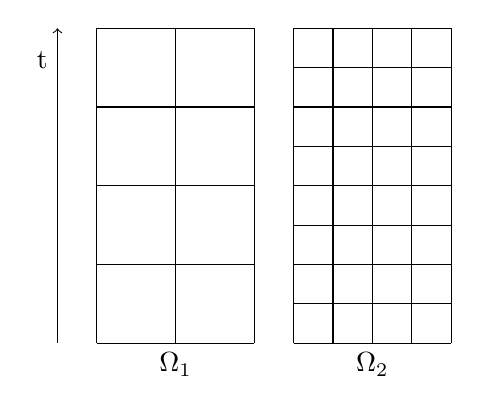
\begin{tikzpicture}
          \draw[<-] (-.5,4) -- (-.5,0) node[pos=.1,left] {t};
          \draw (0,0) grid (2,4);
          \draw (1,0) node[below] {$\Omega_1$};
          \draw[step=.5] (2.499,0) grid (4.5,4);
          \draw (3.5,0) node[below] {$\Omega_2$};
        \end{tikzpicture}
      \end{figure}

    \end{column}
  \end{columns}
\end{frame}


\begin{frame}{Schwarz Waveform Relaxation (SWR)}

  Advantages of SWR
  \begin{itemize}
  \item Reduced communication cost
  \item Naturally handles different discretizations in time
  \item Ideal for multiphysics
  \item Ideal for multiscale
  \end{itemize}

\end{frame}



\section{Pipeline Schwarz Waveform Relaxation}

\subsection{Intuition}

\begin{frame}
  \frametitle{Pipeline Schwarz Waveform Relaxation (animation)}
  \only<1>{
  \begin{figure}
    \centering
    \definecolor{darkgreen}{rgb}{0,.6,0}
  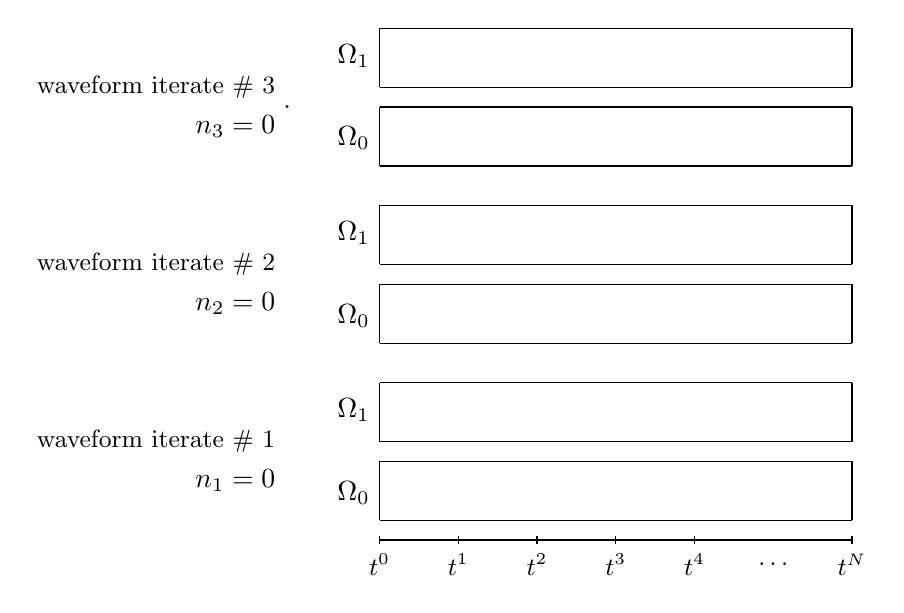
\begin{tikzpicture}[scale=1.0]

    \tikzstyle{dropline_style}=[densely dotted,thin]

    %\foreach \x/\xtext in {-1, -0.5/-\frac{1}{2}, 1}
    %\draw (\x cm,1pt) -- (\x cm,-1pt) node[anchor=north] {$\xtext$};

    \draw(-2,5) node[left] {.};
    \draw (-2.2, 0.75) node[left] {\small waveform iterate \# 1};
    \draw (-2.2, 3) node[left] {\small waveform iterate \# 2};
    \draw (-2.2, 5.25) node[left] {\small waveform iterate \# 3};

    \draw (-2.2, 0.25) node[left] {$n_1=0$};
    \draw (-2.2, 2.5) node[left] {$n_2=0$};
    \draw (-2.2, 4.75) node[left] {$n_3=0$};



    \def\a{-0.25}
    \def\b{0.5}
    \draw (-1,\a) -- (5,\a);
    \draw (5,\a) -- (5,\b);
    \draw (5,\b) -- (-1,\b);
    \draw (-1,\b) -- (-1,\a);

    \def\c{0.75}
    \def\d{1.5}
    \draw (-1,\c) -- (5,\c);
    \draw (5,\c) -- (5,\d);
    \draw (5,\d) -- (-1,\d);
    \draw (-1,\d) -- (-1,\c);

    \draw(-1,0.1) node[left] {$\Omega_0$};
    \draw(-1,1.15) node[left] {$\Omega_1$};

    \def\e{2}
    \def\f{2.75}
    \draw (-1,\e) -- (5,\e);
    \draw (5,\e) -- (5,\f);
    \draw (5,\f) -- (-1,\f);
    \draw (-1,\f) -- (-1,\e);

    \def\g{3}
    \def\h{3.75}
    \draw (-1,\g) -- (5,\g);
    \draw (5,\g) -- (5,\h);
    \draw (5,\h) -- (-1,\h);
    \draw (-1,\h) -- (-1,\g);

    \draw(-1,2.35) node[left] {$\Omega_0$};
    \draw(-1,3.4) node[left] {$\Omega_1$};

    \def\i{4.25}
    \def\j{5}
    \draw (-1,\i) -- (5,\i);
    \draw (5,\i) -- (5,\j);
    \draw (5,\j) -- (-1,\j);
    \draw (-1,\j) -- (-1,\i);

    \def\k{5.25}
    \def\l{6}
    \draw (-1,\k) -- (5,\k);
    \draw (5,\k) -- (5,\l);
    \draw (5,\l) -- (-1,\l);
    \draw (-1,\l) -- (-1,\k);

    \draw(-1,4.6) node[left] {$\Omega_0$};
    \draw(-1,5.65) node[left] {$\Omega_1$};


    % position of the time-line
    \def\y{-0.5}
    \draw [-] (-1,\y) -- (5,\y);

    \def\tick{0.05}
    \draw (-1,\y) ++(0,\tick) -- ++(0,-2*\tick) node[below] {\small $t^{0}$};
    \draw (0,\y) ++(0,\tick) -- ++(0,-2*\tick) node[below] {\small $t^{1}$};
    \draw (1,\y) ++(0,\tick) -- ++(0,-2*\tick) node[below] {\small $t^{2}$};
    \draw (2,\y) ++(0,\tick) -- ++(0,-2*\tick) node[below] {\small $t^{3}$};
    \draw (3,\y) ++(0,\tick) -- ++(0,-2*\tick) node[below] {\small $t^{4}$};
    \draw (4,\y)  node[below] {\small \phantom{t}$\ldots$\phantom{t}};  
    \draw (5,\y) ++(0,\tick) -- ++(0,-2*\tick) node[below] {\small $t^{N}$};
  
    % parameters for stencil diagrams
    \def\rad{0.12}
    \def\omr{0.88}   % 1-rad
    \def\intthick{0.068}   % thickness of integral bars

    %\draw [-latex,thick,blue] (2,0.2) -- (3,0.2);
    %\draw [-latex,thick,blue] (2,1.2) -- (3,1.2);

    %\draw [-,thick,black] (0,\a) -- (0,\b);
    %\draw [-,thick,black] (0,\c) -- (0,\d);

    %\draw (4,0.45)  node[below] {\small \phantom{t}$\ldots$\phantom{t}};  
    %\draw (4,1.45)  node[below] {\small \phantom{t}$\ldots$\phantom{t}};  
    
  \end{tikzpicture}

  \end{figure}
  }
  \only<2>{
  \begin{figure}
    \centering
    \definecolor{darkgreen}{rgb}{0,.6,0}
  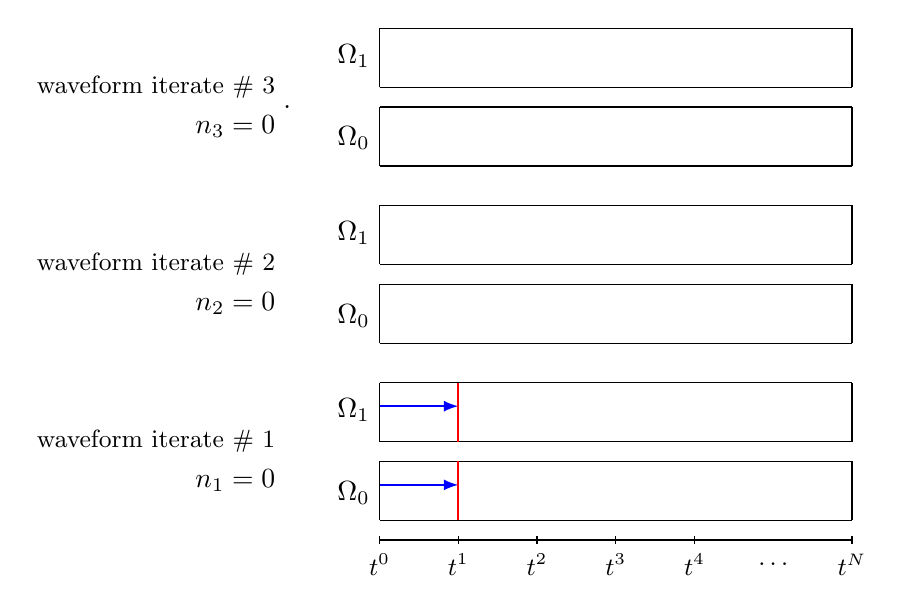
\begin{tikzpicture}[scale=1.0]

    \tikzstyle{dropline_style}=[densely dotted,thin]

    %\foreach \x/\xtext in {-1, -0.5/-\frac{1}{2}, 1}
    %\draw (\x cm,1pt) -- (\x cm,-1pt) node[anchor=north] {$\xtext$};

    \draw(-2,5) node[left] {.};
    \draw (-2.2, 0.75) node[left] {\small waveform iterate \# 1};
    \draw (-2.2, 3) node[left] {\small waveform iterate \# 2};
    \draw (-2.2, 5.25) node[left] {\small waveform iterate \# 3};

    \draw (-2.2, 0.25) node[left] {$n_1=0$};
    \draw (-2.2, 2.5) node[left] {$n_2=0$};
    \draw (-2.2, 4.75) node[left] {$n_3=0$};



    \def\a{-0.25}
    \def\b{0.5}
    \draw (-1,\a) -- (5,\a);
    \draw (5,\a) -- (5,\b);
    \draw (5,\b) -- (-1,\b);
    \draw (-1,\b) -- (-1,\a);

    \def\c{0.75}
    \def\d{1.5}
    \draw (-1,\c) -- (5,\c);
    \draw (5,\c) -- (5,\d);
    \draw (5,\d) -- (-1,\d);
    \draw (-1,\d) -- (-1,\c);

    \draw(-1,0.1) node[left] {$\Omega_0$};
    \draw(-1,1.15) node[left] {$\Omega_1$};

    \def\e{2}
    \def\f{2.75}
    \draw (-1,\e) -- (5,\e);
    \draw (5,\e) -- (5,\f);
    \draw (5,\f) -- (-1,\f);
    \draw (-1,\f) -- (-1,\e);

    \def\g{3}
    \def\h{3.75}
    \draw (-1,\g) -- (5,\g);
    \draw (5,\g) -- (5,\h);
    \draw (5,\h) -- (-1,\h);
    \draw (-1,\h) -- (-1,\g);

    \draw(-1,2.35) node[left] {$\Omega_0$};
    \draw(-1,3.4) node[left] {$\Omega_1$};

    \def\i{4.25}
    \def\j{5}
    \draw (-1,\i) -- (5,\i);
    \draw (5,\i) -- (5,\j);
    \draw (5,\j) -- (-1,\j);
    \draw (-1,\j) -- (-1,\i);

    \def\k{5.25}
    \def\l{6}
    \draw (-1,\k) -- (5,\k);
    \draw (5,\k) -- (5,\l);
    \draw (5,\l) -- (-1,\l);
    \draw (-1,\l) -- (-1,\k);

    \draw(-1,4.6) node[left] {$\Omega_0$};
    \draw(-1,5.65) node[left] {$\Omega_1$};


    % position of the time-line
    \def\y{-0.5}
    \draw [-] (-1,\y) -- (5,\y);

    \def\tick{0.05}
    \draw (-1,\y) ++(0,\tick) -- ++(0,-2*\tick) node[below] {\small $t^{0}$};
    \draw (0,\y) ++(0,\tick) -- ++(0,-2*\tick) node[below] {\small $t^{1}$};
    \draw (1,\y) ++(0,\tick) -- ++(0,-2*\tick) node[below] {\small $t^{2}$};
    \draw (2,\y) ++(0,\tick) -- ++(0,-2*\tick) node[below] {\small $t^{3}$};
    \draw (3,\y) ++(0,\tick) -- ++(0,-2*\tick) node[below] {\small $t^{4}$};
    \draw (4,\y)  node[below] {\small \phantom{t}$\ldots$\phantom{t}};  
    \draw (5,\y) ++(0,\tick) -- ++(0,-2*\tick) node[below] {\small $t^{N}$};
  
    % parameters for stencil diagrams
    \def\rad{0.12}
    \def\omr{0.88}   % 1-rad
    \def\intthick{0.068}   % thickness of integral bars

    \draw [-latex,thick,blue] (-1,0.2) -- (0,0.2);
    \draw [-latex,thick,blue] (-1,1.2) -- (0,1.2);

    \draw [-,thick,red] (0,\a) -- (0,\b);
    \draw [-,thick,red] (0,\c) -- (0,\d);

    %\draw (4,0.45)  node[below] {\small \phantom{t}$\ldots$\phantom{t}};  
    %\draw (4,1.45)  node[below] {\small \phantom{t}$\ldots$\phantom{t}};  
    
  \end{tikzpicture}

  \end{figure}
  }
  \only<3>{
  \begin{figure}
    \centering
    \definecolor{darkgreen}{rgb}{0,.6,0}
  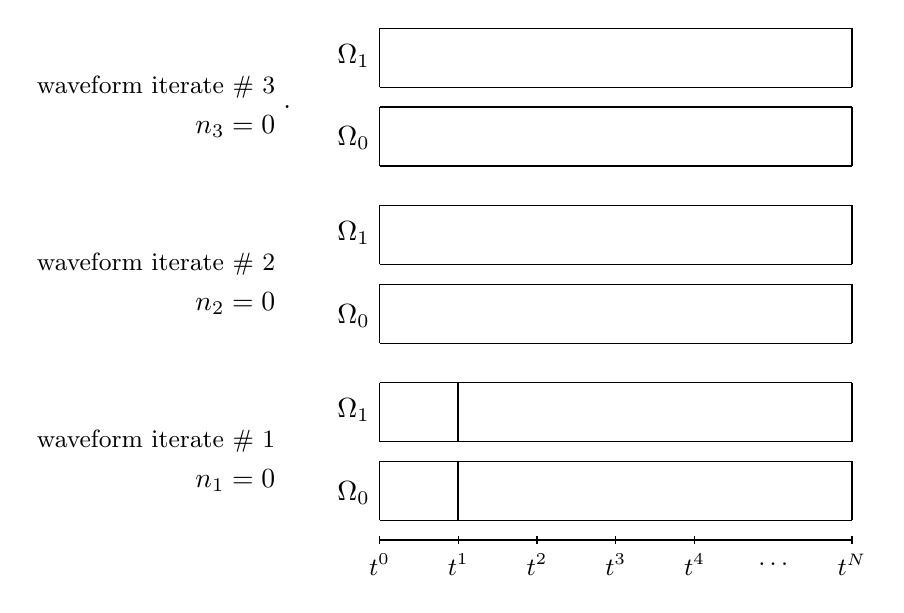
\begin{tikzpicture}[scale=1.0]

    \tikzstyle{dropline_style}=[densely dotted,thin]

    %\foreach \x/\xtext in {-1, -0.5/-\frac{1}{2}, 1}
    %\draw (\x cm,1pt) -- (\x cm,-1pt) node[anchor=north] {$\xtext$};

    \draw(-2,5) node[left] {.};
    \draw (-2.2, 0.75) node[left] {\small waveform iterate \# 1};
    \draw (-2.2, 3) node[left] {\small waveform iterate \# 2};
    \draw (-2.2, 5.25) node[left] {\small waveform iterate \# 3};

    \draw (-2.2, 0.25) node[left] {$n_1=0$};
    \draw (-2.2, 2.5) node[left] {$n_2=0$};
    \draw (-2.2, 4.75) node[left] {$n_3=0$};



    \def\a{-0.25}
    \def\b{0.5}
    \draw (-1,\a) -- (5,\a);
    \draw (5,\a) -- (5,\b);
    \draw (5,\b) -- (-1,\b);
    \draw (-1,\b) -- (-1,\a);

    \def\c{0.75}
    \def\d{1.5}
    \draw (-1,\c) -- (5,\c);
    \draw (5,\c) -- (5,\d);
    \draw (5,\d) -- (-1,\d);
    \draw (-1,\d) -- (-1,\c);

    \draw(-1,0.1) node[left] {$\Omega_0$};
    \draw(-1,1.15) node[left] {$\Omega_1$};

    \def\e{2}
    \def\f{2.75}
    \draw (-1,\e) -- (5,\e);
    \draw (5,\e) -- (5,\f);
    \draw (5,\f) -- (-1,\f);
    \draw (-1,\f) -- (-1,\e);

    \def\g{3}
    \def\h{3.75}
    \draw (-1,\g) -- (5,\g);
    \draw (5,\g) -- (5,\h);
    \draw (5,\h) -- (-1,\h);
    \draw (-1,\h) -- (-1,\g);

    \draw(-1,2.35) node[left] {$\Omega_0$};
    \draw(-1,3.4) node[left] {$\Omega_1$};

    \def\i{4.25}
    \def\j{5}
    \draw (-1,\i) -- (5,\i);
    \draw (5,\i) -- (5,\j);
    \draw (5,\j) -- (-1,\j);
    \draw (-1,\j) -- (-1,\i);

    \def\k{5.25}
    \def\l{6}
    \draw (-1,\k) -- (5,\k);
    \draw (5,\k) -- (5,\l);
    \draw (5,\l) -- (-1,\l);
    \draw (-1,\l) -- (-1,\k);

    \draw(-1,4.6) node[left] {$\Omega_0$};
    \draw(-1,5.65) node[left] {$\Omega_1$};


    % position of the time-line
    \def\y{-0.5}
    \draw [-] (-1,\y) -- (5,\y);

    \def\tick{0.05}
    \draw (-1,\y) ++(0,\tick) -- ++(0,-2*\tick) node[below] {\small $t^{0}$};
    \draw (0,\y) ++(0,\tick) -- ++(0,-2*\tick) node[below] {\small $t^{1}$};
    \draw (1,\y) ++(0,\tick) -- ++(0,-2*\tick) node[below] {\small $t^{2}$};
    \draw (2,\y) ++(0,\tick) -- ++(0,-2*\tick) node[below] {\small $t^{3}$};
    \draw (3,\y) ++(0,\tick) -- ++(0,-2*\tick) node[below] {\small $t^{4}$};
    \draw (4,\y)  node[below] {\small \phantom{t}$\ldots$\phantom{t}};  
    \draw (5,\y) ++(0,\tick) -- ++(0,-2*\tick) node[below] {\small $t^{N}$};
  
    % parameters for stencil diagrams
    \def\rad{0.12}
    \def\omr{0.88}   % 1-rad
    \def\intthick{0.068}   % thickness of integral bars

    %\draw [-latex,thick,blue] (-1,0.2) -- (0,0.2);
    %\draw [-latex,thick,blue] (-1,1.2) -- (0,1.2);

    \draw [-,thick,black] (0,\a) -- (0,\b);
    \draw [-,thick,black] (0,\c) -- (0,\d);

    %\draw (4,0.45)  node[below] {\small \phantom{t}$\ldots$\phantom{t}};  
    %\draw (4,1.45)  node[below] {\small \phantom{t}$\ldots$\phantom{t}};  
    
  \end{tikzpicture}

  \end{figure}
  }
  \only<4>{
  \begin{figure}
    \centering
    \definecolor{darkgreen}{rgb}{0,.6,0}
  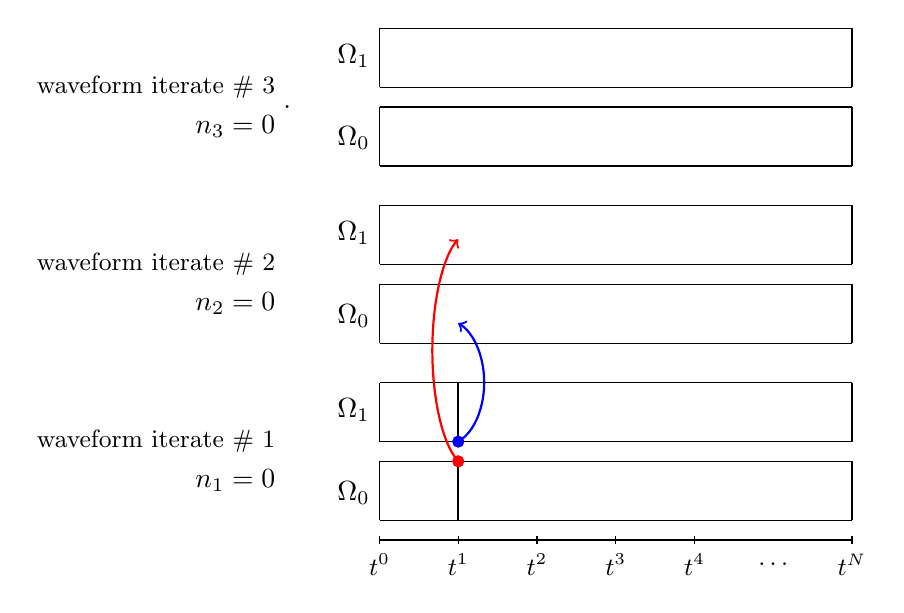
\begin{tikzpicture}[scale=1.0]

    \tikzstyle{dropline_style}=[densely dotted,thin]

    %\foreach \x/\xtext in {-1, -0.5/-\frac{1}{2}, 1}
    %\draw (\x cm,1pt) -- (\x cm,-1pt) node[anchor=north] {$\xtext$};

    \draw(-2,5) node[left] {.};
    \draw (-2.2, 0.75) node[left] {\small waveform iterate \# 1};
    \draw (-2.2, 3) node[left] {\small waveform iterate \# 2};
    \draw (-2.2, 5.25) node[left] {\small waveform iterate \# 3};

    \draw (-2.2, 0.25) node[left] {$n_1=0$};
    \draw (-2.2, 2.5) node[left] {$n_2=0$};
    \draw (-2.2, 4.75) node[left] {$n_3=0$};



    \def\a{-0.25}
    \def\b{0.5}
    \draw (-1,\a) -- (5,\a);
    \draw (5,\a) -- (5,\b);
    \draw (5,\b) -- (-1,\b);
    \draw (-1,\b) -- (-1,\a);

    \def\c{0.75}
    \def\d{1.5}
    \draw (-1,\c) -- (5,\c);
    \draw (5,\c) -- (5,\d);
    \draw (5,\d) -- (-1,\d);
    \draw (-1,\d) -- (-1,\c);

    \draw(-1,0.1) node[left] {$\Omega_0$};
    \draw(-1,1.15) node[left] {$\Omega_1$};

    \def\e{2}
    \def\f{2.75}
    \draw (-1,\e) -- (5,\e);
    \draw (5,\e) -- (5,\f);
    \draw (5,\f) -- (-1,\f);
    \draw (-1,\f) -- (-1,\e);

    \def\g{3}
    \def\h{3.75}
    \draw (-1,\g) -- (5,\g);
    \draw (5,\g) -- (5,\h);
    \draw (5,\h) -- (-1,\h);
    \draw (-1,\h) -- (-1,\g);

    \draw(-1,2.35) node[left] {$\Omega_0$};
    \draw(-1,3.4) node[left] {$\Omega_1$};

    \def\i{4.25}
    \def\j{5}
    \draw (-1,\i) -- (5,\i);
    \draw (5,\i) -- (5,\j);
    \draw (5,\j) -- (-1,\j);
    \draw (-1,\j) -- (-1,\i);

    \def\k{5.25}
    \def\l{6}
    \draw (-1,\k) -- (5,\k);
    \draw (5,\k) -- (5,\l);
    \draw (5,\l) -- (-1,\l);
    \draw (-1,\l) -- (-1,\k);

    \draw(-1,4.6) node[left] {$\Omega_0$};
    \draw(-1,5.65) node[left] {$\Omega_1$};


    % position of the time-line
    \def\y{-0.5}
    \draw [-] (-1,\y) -- (5,\y);

    \def\tick{0.05}
    \draw (-1,\y) ++(0,\tick) -- ++(0,-2*\tick) node[below] {\small $t^{0}$};
    \draw (0,\y) ++(0,\tick) -- ++(0,-2*\tick) node[below] {\small $t^{1}$};
    \draw (1,\y) ++(0,\tick) -- ++(0,-2*\tick) node[below] {\small $t^{2}$};
    \draw (2,\y) ++(0,\tick) -- ++(0,-2*\tick) node[below] {\small $t^{3}$};
    \draw (3,\y) ++(0,\tick) -- ++(0,-2*\tick) node[below] {\small $t^{4}$};
    \draw (4,\y)  node[below] {\small \phantom{t}$\ldots$\phantom{t}};  
    \draw (5,\y) ++(0,\tick) -- ++(0,-2*\tick) node[below] {\small $t^{N}$};
  
    % parameters for stencil diagrams
    \def\rad{0.12}
    \def\omr{0.88}   % 1-rad
    \def\intthick{0.068}   % thickness of integral bars

    %\draw [-latex,thick,blue] (-1,0.2) -- (0,0.2);
    %\draw [-latex,thick,blue] (-1,1.2) -- (0,1.2);

    \draw [-,thick,black] (0,\a) -- (0,\b);
    \draw [-,thick,black] (0,\c) -- (0,\d);

    %\draw (4,0.45)  node[below] {\small \phantom{t}$\ldots$\phantom{t}};  
    %\draw (4,1.45)  node[below] {\small \phantom{t}$\ldots$\phantom{t}};  
    
    % filled dots
    \foreach \xy in { (0,\b)}
    \filldraw [red] \xy circle (2pt);

    \foreach \xy in { (0,\c)}
    \filldraw [blue] \xy circle (2pt);


    \draw [->,thick,red] (0,0.5) arc (250:110:0.5 and 1.5);
    \draw [->,thick,blue] (0,0.75) arc (-70:70:0.5 and 0.8);

  \end{tikzpicture}

  \end{figure}
  }
  \only<5>{
  \begin{figure}
    \centering
    \definecolor{darkgreen}{rgb}{0,.6,0}
  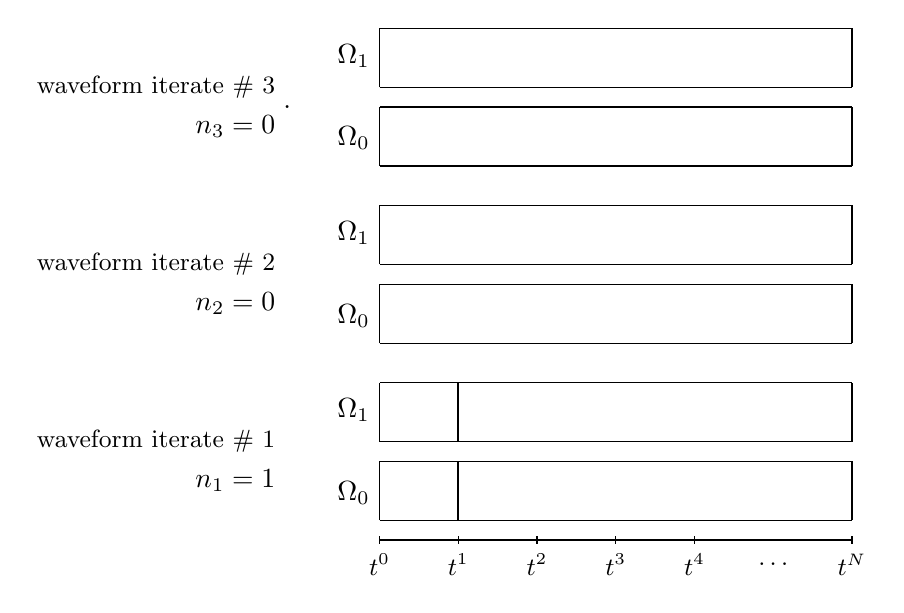
\begin{tikzpicture}[scale=1.0]

    \tikzstyle{dropline_style}=[densely dotted,thin]

    %\foreach \x/\xtext in {-1, -0.5/-\frac{1}{2}, 1}
    %\draw (\x cm,1pt) -- (\x cm,-1pt) node[anchor=north] {$\xtext$};

    \draw(-2,5) node[left] {.};
    \draw (-2.2, 0.75) node[left] {\small waveform iterate \# 1};
    \draw (-2.2, 3) node[left] {\small waveform iterate \# 2};
    \draw (-2.2, 5.25) node[left] {\small waveform iterate \# 3};

    \draw (-2.2, 0.25) node[left] {$n_1=1$};
    \draw (-2.2, 2.5) node[left] {$n_2=0$};
    \draw (-2.2, 4.75) node[left] {$n_3=0$};



    \def\a{-0.25}
    \def\b{0.5}
    \draw (-1,\a) -- (5,\a);
    \draw (5,\a) -- (5,\b);
    \draw (5,\b) -- (-1,\b);
    \draw (-1,\b) -- (-1,\a);

    \def\c{0.75}
    \def\d{1.5}
    \draw (-1,\c) -- (5,\c);
    \draw (5,\c) -- (5,\d);
    \draw (5,\d) -- (-1,\d);
    \draw (-1,\d) -- (-1,\c);

    \draw(-1,0.1) node[left] {$\Omega_0$};
    \draw(-1,1.15) node[left] {$\Omega_1$};

    \def\e{2}
    \def\f{2.75}
    \draw (-1,\e) -- (5,\e);
    \draw (5,\e) -- (5,\f);
    \draw (5,\f) -- (-1,\f);
    \draw (-1,\f) -- (-1,\e);

    \def\g{3}
    \def\h{3.75}
    \draw (-1,\g) -- (5,\g);
    \draw (5,\g) -- (5,\h);
    \draw (5,\h) -- (-1,\h);
    \draw (-1,\h) -- (-1,\g);

    \draw(-1,2.35) node[left] {$\Omega_0$};
    \draw(-1,3.4) node[left] {$\Omega_1$};

    \def\i{4.25}
    \def\j{5}
    \draw (-1,\i) -- (5,\i);
    \draw (5,\i) -- (5,\j);
    \draw (5,\j) -- (-1,\j);
    \draw (-1,\j) -- (-1,\i);

    \def\k{5.25}
    \def\l{6}
    \draw (-1,\k) -- (5,\k);
    \draw (5,\k) -- (5,\l);
    \draw (5,\l) -- (-1,\l);
    \draw (-1,\l) -- (-1,\k);

    \draw(-1,4.6) node[left] {$\Omega_0$};
    \draw(-1,5.65) node[left] {$\Omega_1$};


    % position of the time-line
    \def\y{-0.5}
    \draw [-] (-1,\y) -- (5,\y);

    \def\tick{0.05}
    \draw (-1,\y) ++(0,\tick) -- ++(0,-2*\tick) node[below] {\small $t^{0}$};
    \draw (0,\y) ++(0,\tick) -- ++(0,-2*\tick) node[below] {\small $t^{1}$};
    \draw (1,\y) ++(0,\tick) -- ++(0,-2*\tick) node[below] {\small $t^{2}$};
    \draw (2,\y) ++(0,\tick) -- ++(0,-2*\tick) node[below] {\small $t^{3}$};
    \draw (3,\y) ++(0,\tick) -- ++(0,-2*\tick) node[below] {\small $t^{4}$};
    \draw (4,\y)  node[below] {\small \phantom{t}$\ldots$\phantom{t}};  
    \draw (5,\y) ++(0,\tick) -- ++(0,-2*\tick) node[below] {\small $t^{N}$};
  
    % parameters for stencil diagrams
    \def\rad{0.12}
    \def\omr{0.88}   % 1-rad
    \def\intthick{0.068}   % thickness of integral bars

    %\draw [-latex,thick,blue] (-1,0.2) -- (0,0.2);
    %\draw [-latex,thick,blue] (-1,1.2) -- (0,1.2);

    \draw [-,thick,black] (0,\a) -- (0,\b);
    \draw [-,thick,black] (0,\c) -- (0,\d);

    %\draw (4,0.45)  node[below] {\small \phantom{t}$\ldots$\phantom{t}};  
    %\draw (4,1.45)  node[below] {\small \phantom{t}$\ldots$\phantom{t}};  
    
    % filled dots
    %\foreach \xy in { (0,\b)}
    %\filldraw [red] \xy circle (2pt);

    %\foreach \xy in { (0,\c)}
    %\filldraw [blue] \xy circle (2pt);


    %\draw [->,thick,red] (0,0.5) arc (250:110:0.5 and 1.5);
    %\draw [->,thick,blue] (0,0.75) arc (-70:70:0.5 and 0.8);

  \end{tikzpicture}

  \end{figure}
  }
  \only<6>{
  \begin{figure}
    \centering
    \definecolor{darkgreen}{rgb}{0,.6,0}
  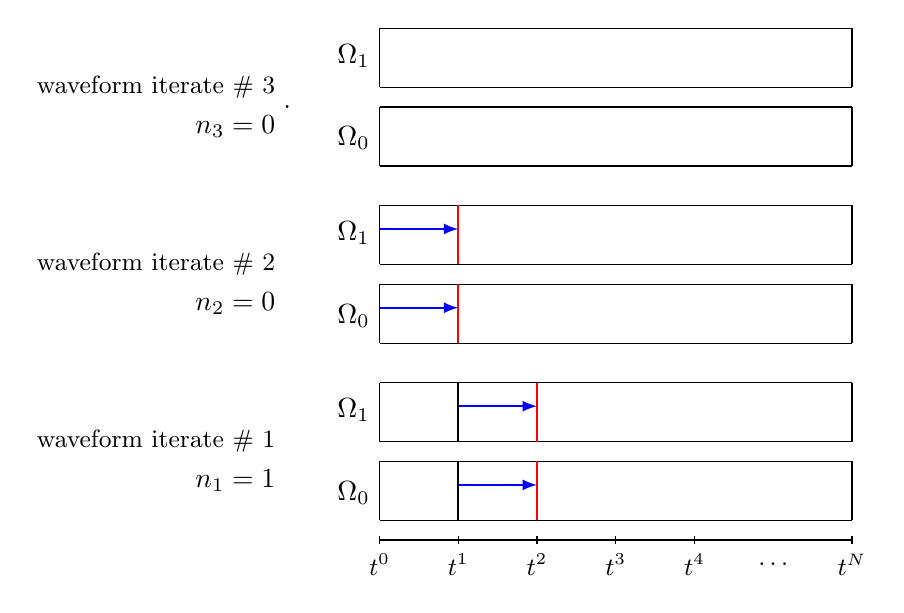
\begin{tikzpicture}[scale=1.0]

    \tikzstyle{dropline_style}=[densely dotted,thin]

    %\foreach \x/\xtext in {-1, -0.5/-\frac{1}{2}, 1}
    %\draw (\x cm,1pt) -- (\x cm,-1pt) node[anchor=north] {$\xtext$};

    \draw(-2,5) node[left] {.};
    \draw (-2.2, 0.75) node[left] {\small waveform iterate \# 1};
    \draw (-2.2, 3) node[left] {\small waveform iterate \# 2};
    \draw (-2.2, 5.25) node[left] {\small waveform iterate \# 3};

    \draw (-2.2, 0.25) node[left] {$n_1=1$};
    \draw (-2.2, 2.5) node[left] {$n_2=0$};
    \draw (-2.2, 4.75) node[left] {$n_3=0$};



    \def\a{-0.25}
    \def\b{0.5}
    \draw (-1,\a) -- (5,\a);
    \draw (5,\a) -- (5,\b);
    \draw (5,\b) -- (-1,\b);
    \draw (-1,\b) -- (-1,\a);

    \def\c{0.75}
    \def\d{1.5}
    \draw (-1,\c) -- (5,\c);
    \draw (5,\c) -- (5,\d);
    \draw (5,\d) -- (-1,\d);
    \draw (-1,\d) -- (-1,\c);

    \draw(-1,0.1) node[left] {$\Omega_0$};
    \draw(-1,1.15) node[left] {$\Omega_1$};

    \def\e{2}
    \def\f{2.75}
    \draw (-1,\e) -- (5,\e);
    \draw (5,\e) -- (5,\f);
    \draw (5,\f) -- (-1,\f);
    \draw (-1,\f) -- (-1,\e);

    \def\g{3}
    \def\h{3.75}
    \draw (-1,\g) -- (5,\g);
    \draw (5,\g) -- (5,\h);
    \draw (5,\h) -- (-1,\h);
    \draw (-1,\h) -- (-1,\g);

    \draw(-1,2.35) node[left] {$\Omega_0$};
    \draw(-1,3.4) node[left] {$\Omega_1$};

    \def\i{4.25}
    \def\j{5}
    \draw (-1,\i) -- (5,\i);
    \draw (5,\i) -- (5,\j);
    \draw (5,\j) -- (-1,\j);
    \draw (-1,\j) -- (-1,\i);

    \def\k{5.25}
    \def\l{6}
    \draw (-1,\k) -- (5,\k);
    \draw (5,\k) -- (5,\l);
    \draw (5,\l) -- (-1,\l);
    \draw (-1,\l) -- (-1,\k);

    \draw(-1,4.6) node[left] {$\Omega_0$};
    \draw(-1,5.65) node[left] {$\Omega_1$};


    % position of the time-line
    \def\y{-0.5}
    \draw [-] (-1,\y) -- (5,\y);

    \def\tick{0.05}
    \draw (-1,\y) ++(0,\tick) -- ++(0,-2*\tick) node[below] {\small $t^{0}$};
    \draw (0,\y) ++(0,\tick) -- ++(0,-2*\tick) node[below] {\small $t^{1}$};
    \draw (1,\y) ++(0,\tick) -- ++(0,-2*\tick) node[below] {\small $t^{2}$};
    \draw (2,\y) ++(0,\tick) -- ++(0,-2*\tick) node[below] {\small $t^{3}$};
    \draw (3,\y) ++(0,\tick) -- ++(0,-2*\tick) node[below] {\small $t^{4}$};
    \draw (4,\y)  node[below] {\small \phantom{t}$\ldots$\phantom{t}};  
    \draw (5,\y) ++(0,\tick) -- ++(0,-2*\tick) node[below] {\small $t^{N}$};
  
    % parameters for stencil diagrams
    \def\rad{0.12}
    \def\omr{0.88}   % 1-rad
    \def\intthick{0.068}   % thickness of integral bars

    \draw [-latex,thick,blue] (0,0.2) -- (1,0.2);
    \draw [-latex,thick,blue] (0,1.2) -- (1,1.2);

    \draw [-latex,thick,blue] (-1,2.45) -- (0,2.45);
    \draw [-latex,thick,blue] (-1,3.45) -- (0,3.45);

    \draw [-,thick,black] (0,\a) -- (0,\b);
    \draw [-,thick,black] (0,\c) -- (0,\d);

    \draw [-,thick,red] (1,\a) -- (1,\b);
    \draw [-,thick,red] (1,\c) -- (1,\d);

    \draw [-,thick,red] (0,\e) -- (0,\f);
    \draw [-,thick,red] (0,\g) -- (0,\h);

    %\draw (4,0.45)  node[below] {\small \phantom{t}$\ldots$\phantom{t}};  
    %\draw (4,1.45)  node[below] {\small \phantom{t}$\ldots$\phantom{t}};  
    
    % filled dots
    %\foreach \xy in { (0,\b)}
    %\filldraw [red] \xy circle (2pt);

    %\foreach \xy in { (0,\c)}
    %\filldraw [blue] \xy circle (2pt);


    %\draw [->,thick,red] (0,0.5) arc (250:110:0.5 and 1.5);
    %\draw [->,thick,blue] (0,0.75) arc (-70:70:0.5 and 0.8);

  \end{tikzpicture}

  \end{figure}
  }
  \only<7>{
  \begin{figure}
    \centering
    \definecolor{darkgreen}{rgb}{0,.6,0}
  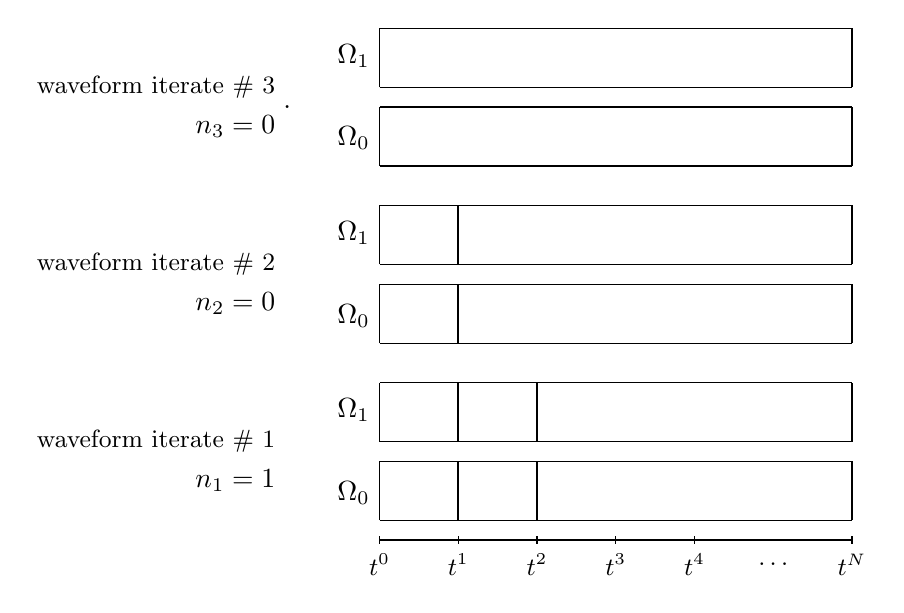
\begin{tikzpicture}[scale=1.0]

    \tikzstyle{dropline_style}=[densely dotted,thin]

    %\foreach \x/\xtext in {-1, -0.5/-\frac{1}{2}, 1}
    %\draw (\x cm,1pt) -- (\x cm,-1pt) node[anchor=north] {$\xtext$};

    \draw(-2,5) node[left] {.};
    \draw (-2.2, 0.75) node[left] {\small waveform iterate \# 1};
    \draw (-2.2, 3) node[left] {\small waveform iterate \# 2};
    \draw (-2.2, 5.25) node[left] {\small waveform iterate \# 3};

    \draw (-2.2, 0.25) node[left] {$n_1=1$};
    \draw (-2.2, 2.5) node[left] {$n_2=0$};
    \draw (-2.2, 4.75) node[left] {$n_3=0$};



    \def\a{-0.25}
    \def\b{0.5}
    \draw (-1,\a) -- (5,\a);
    \draw (5,\a) -- (5,\b);
    \draw (5,\b) -- (-1,\b);
    \draw (-1,\b) -- (-1,\a);

    \def\c{0.75}
    \def\d{1.5}
    \draw (-1,\c) -- (5,\c);
    \draw (5,\c) -- (5,\d);
    \draw (5,\d) -- (-1,\d);
    \draw (-1,\d) -- (-1,\c);

    \draw(-1,0.1) node[left] {$\Omega_0$};
    \draw(-1,1.15) node[left] {$\Omega_1$};

    \def\e{2}
    \def\f{2.75}
    \draw (-1,\e) -- (5,\e);
    \draw (5,\e) -- (5,\f);
    \draw (5,\f) -- (-1,\f);
    \draw (-1,\f) -- (-1,\e);

    \def\g{3}
    \def\h{3.75}
    \draw (-1,\g) -- (5,\g);
    \draw (5,\g) -- (5,\h);
    \draw (5,\h) -- (-1,\h);
    \draw (-1,\h) -- (-1,\g);

    \draw(-1,2.35) node[left] {$\Omega_0$};
    \draw(-1,3.4) node[left] {$\Omega_1$};

    \def\i{4.25}
    \def\j{5}
    \draw (-1,\i) -- (5,\i);
    \draw (5,\i) -- (5,\j);
    \draw (5,\j) -- (-1,\j);
    \draw (-1,\j) -- (-1,\i);

    \def\k{5.25}
    \def\l{6}
    \draw (-1,\k) -- (5,\k);
    \draw (5,\k) -- (5,\l);
    \draw (5,\l) -- (-1,\l);
    \draw (-1,\l) -- (-1,\k);

    \draw(-1,4.6) node[left] {$\Omega_0$};
    \draw(-1,5.65) node[left] {$\Omega_1$};


    % position of the time-line
    \def\y{-0.5}
    \draw [-] (-1,\y) -- (5,\y);

    \def\tick{0.05}
    \draw (-1,\y) ++(0,\tick) -- ++(0,-2*\tick) node[below] {\small $t^{0}$};
    \draw (0,\y) ++(0,\tick) -- ++(0,-2*\tick) node[below] {\small $t^{1}$};
    \draw (1,\y) ++(0,\tick) -- ++(0,-2*\tick) node[below] {\small $t^{2}$};
    \draw (2,\y) ++(0,\tick) -- ++(0,-2*\tick) node[below] {\small $t^{3}$};
    \draw (3,\y) ++(0,\tick) -- ++(0,-2*\tick) node[below] {\small $t^{4}$};
    \draw (4,\y)  node[below] {\small \phantom{t}$\ldots$\phantom{t}};  
    \draw (5,\y) ++(0,\tick) -- ++(0,-2*\tick) node[below] {\small $t^{N}$};
  
    % parameters for stencil diagrams
    \def\rad{0.12}
    \def\omr{0.88}   % 1-rad
    \def\intthick{0.068}   % thickness of integral bars

    %\draw [-latex,thick,blue] (0,0.2) -- (1,0.2);
    %\draw [-latex,thick,blue] (0,1.2) -- (1,1.2);

    %\draw [-latex,thick,blue] (-1,2.45) -- (0,2.45);
    %\draw [-latex,thick,blue] (-1,3.45) -- (0,3.45);

    \draw [-,thick,black] (0,\a) -- (0,\b);
    \draw [-,thick,black] (0,\c) -- (0,\d);

    \draw [-,thick,black] (1,\a) -- (1,\b);
    \draw [-,thick,black] (1,\c) -- (1,\d);

    \draw [-,thick,black] (0,\e) -- (0,\f);
    \draw [-,thick,black] (0,\g) -- (0,\h);

    %\draw (4,0.45)  node[below] {\small \phantom{t}$\ldots$\phantom{t}};  
    %\draw (4,1.45)  node[below] {\small \phantom{t}$\ldots$\phantom{t}};  
    
    % filled dots
    %% \foreach \xy in { (0,\b)}
    %% \filldraw [red] \xy circle (2pt);

    %% \foreach \xy in { (0,\c)}
    %% \filldraw [blue] \xy circle (2pt);

    %% \draw [->,thick,red] (0,0.5) arc (250:110:0.5 and 1.5);
    %% \draw [->,thick,blue] (0,0.75) arc (-70:70:0.5 and 0.8);

  \end{tikzpicture}

  \end{figure}
  }    
  \only<8>{
  \begin{figure}
    \centering
    \definecolor{darkgreen}{rgb}{0,.6,0}
  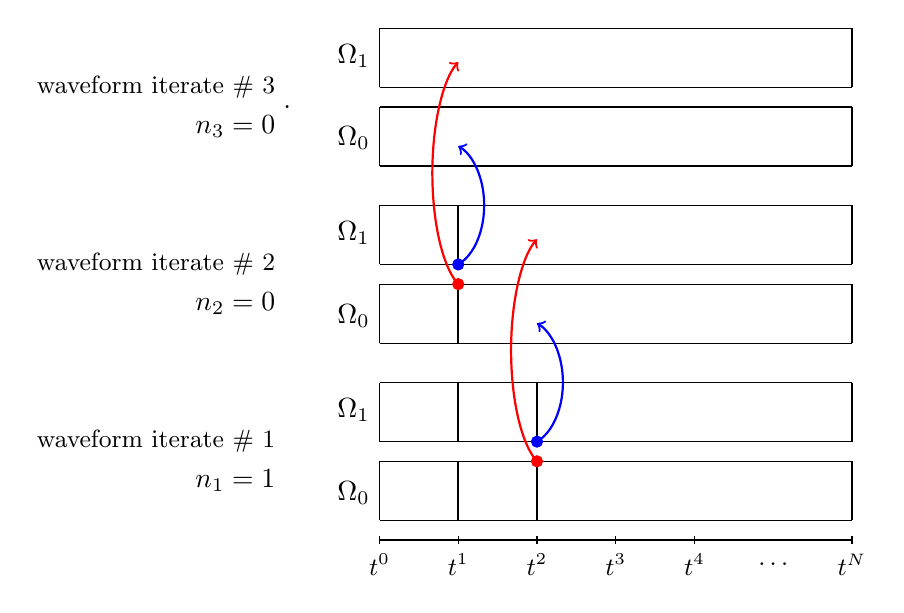
\begin{tikzpicture}[scale=1.0]

    \tikzstyle{dropline_style}=[densely dotted,thin]

    %\foreach \x/\xtext in {-1, -0.5/-\frac{1}{2}, 1}
    %\draw (\x cm,1pt) -- (\x cm,-1pt) node[anchor=north] {$\xtext$};

    \draw(-2,5) node[left] {.};
    \draw (-2.2, 0.75) node[left] {\small waveform iterate \# 1};
    \draw (-2.2, 3) node[left] {\small waveform iterate \# 2};
    \draw (-2.2, 5.25) node[left] {\small waveform iterate \# 3};

    \draw (-2.2, 0.25) node[left] {$n_1=1$};
    \draw (-2.2, 2.5) node[left] {$n_2=0$};
    \draw (-2.2, 4.75) node[left] {$n_3=0$};



    \def\a{-0.25}
    \def\b{0.5}
    \draw (-1,\a) -- (5,\a);
    \draw (5,\a) -- (5,\b);
    \draw (5,\b) -- (-1,\b);
    \draw (-1,\b) -- (-1,\a);

    \def\c{0.75}
    \def\d{1.5}
    \draw (-1,\c) -- (5,\c);
    \draw (5,\c) -- (5,\d);
    \draw (5,\d) -- (-1,\d);
    \draw (-1,\d) -- (-1,\c);

    \draw(-1,0.1) node[left] {$\Omega_0$};
    \draw(-1,1.15) node[left] {$\Omega_1$};

    \def\e{2}
    \def\f{2.75}
    \draw (-1,\e) -- (5,\e);
    \draw (5,\e) -- (5,\f);
    \draw (5,\f) -- (-1,\f);
    \draw (-1,\f) -- (-1,\e);

    \def\g{3}
    \def\h{3.75}
    \draw (-1,\g) -- (5,\g);
    \draw (5,\g) -- (5,\h);
    \draw (5,\h) -- (-1,\h);
    \draw (-1,\h) -- (-1,\g);

    \draw(-1,2.35) node[left] {$\Omega_0$};
    \draw(-1,3.4) node[left] {$\Omega_1$};

    \def\i{4.25}
    \def\j{5}
    \draw (-1,\i) -- (5,\i);
    \draw (5,\i) -- (5,\j);
    \draw (5,\j) -- (-1,\j);
    \draw (-1,\j) -- (-1,\i);

    \def\k{5.25}
    \def\l{6}
    \draw (-1,\k) -- (5,\k);
    \draw (5,\k) -- (5,\l);
    \draw (5,\l) -- (-1,\l);
    \draw (-1,\l) -- (-1,\k);

    \draw(-1,4.6) node[left] {$\Omega_0$};
    \draw(-1,5.65) node[left] {$\Omega_1$};


    % position of the time-line
    \def\y{-0.5}
    \draw [-] (-1,\y) -- (5,\y);

    \def\tick{0.05}
    \draw (-1,\y) ++(0,\tick) -- ++(0,-2*\tick) node[below] {\small $t^{0}$};
    \draw (0,\y) ++(0,\tick) -- ++(0,-2*\tick) node[below] {\small $t^{1}$};
    \draw (1,\y) ++(0,\tick) -- ++(0,-2*\tick) node[below] {\small $t^{2}$};
    \draw (2,\y) ++(0,\tick) -- ++(0,-2*\tick) node[below] {\small $t^{3}$};
    \draw (3,\y) ++(0,\tick) -- ++(0,-2*\tick) node[below] {\small $t^{4}$};
    \draw (4,\y)  node[below] {\small \phantom{t}$\ldots$\phantom{t}};  
    \draw (5,\y) ++(0,\tick) -- ++(0,-2*\tick) node[below] {\small $t^{N}$};
  
    % parameters for stencil diagrams
    \def\rad{0.12}
    \def\omr{0.88}   % 1-rad
    \def\intthick{0.068}   % thickness of integral bars

    %\draw [-latex,thick,blue] (0,0.2) -- (1,0.2);
    %\draw [-latex,thick,blue] (0,1.2) -- (1,1.2);

    %\draw [-latex,thick,blue] (-1,2.45) -- (0,2.45);
    %\draw [-latex,thick,blue] (-1,3.45) -- (0,3.45);

    \draw [-,thick,black] (0,\a) -- (0,\b);
    \draw [-,thick,black] (0,\c) -- (0,\d);

    \draw [-,thick,black] (1,\a) -- (1,\b);
    \draw [-,thick,black] (1,\c) -- (1,\d);

    \draw [-,thick,black] (0,\e) -- (0,\f);
    \draw [-,thick,black] (0,\g) -- (0,\h);

    %\draw (4,0.45)  node[below] {\small \phantom{t}$\ldots$\phantom{t}};  
    %\draw (4,1.45)  node[below] {\small \phantom{t}$\ldots$\phantom{t}};  
    
    % filled dots
    \foreach \xy in { (1,\b)}
    \filldraw [red] \xy circle (2pt);

    \foreach \xy in { (1,\c)}
    \filldraw [blue] \xy circle (2pt);

    \draw [->,thick,red] (1,0.5) arc (250:110:0.5 and 1.5);
    \draw [->,thick,blue] (1,0.75) arc (-70:70:0.5 and 0.8);

    \foreach \xy in { (0,\f)}
    \filldraw [red] \xy circle (2pt);

    \foreach \xy in { (0,\g)}
    \filldraw [blue] \xy circle (2pt);

    \draw [->,thick,red] (0,2.75) arc (250:110:0.5 and 1.5);
    \draw [->,thick,blue] (0,3) arc (-70:70:0.5 and 0.8);

  \end{tikzpicture}

  \end{figure}
  }    
  \only<9>{
  \begin{figure}
    \centering
    \definecolor{darkgreen}{rgb}{0,.6,0}
  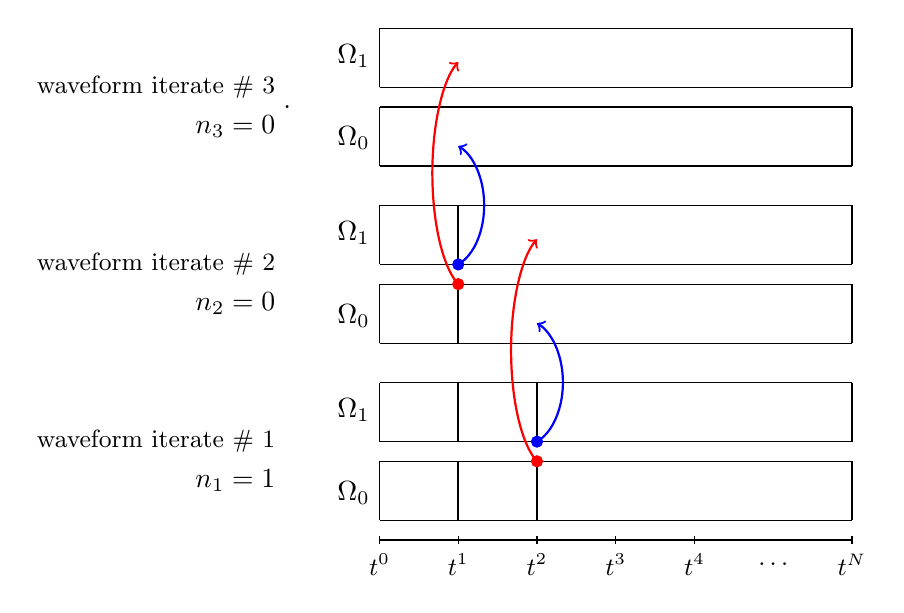
\begin{tikzpicture}[scale=1.0]

    \tikzstyle{dropline_style}=[densely dotted,thin]

    %\foreach \x/\xtext in {-1, -0.5/-\frac{1}{2}, 1}
    %\draw (\x cm,1pt) -- (\x cm,-1pt) node[anchor=north] {$\xtext$};

    \draw(-2,5) node[left] {.};
    \draw (-2.2, 0.75) node[left] {\small waveform iterate \# 1};
    \draw (-2.2, 3) node[left] {\small waveform iterate \# 2};
    \draw (-2.2, 5.25) node[left] {\small waveform iterate \# 3};

    \draw (-2.2, 0.25) node[left] {$n_1=1$};
    \draw (-2.2, 2.5) node[left] {$n_2=0$};
    \draw (-2.2, 4.75) node[left] {$n_3=0$};



    \def\a{-0.25}
    \def\b{0.5}
    \draw (-1,\a) -- (5,\a);
    \draw (5,\a) -- (5,\b);
    \draw (5,\b) -- (-1,\b);
    \draw (-1,\b) -- (-1,\a);

    \def\c{0.75}
    \def\d{1.5}
    \draw (-1,\c) -- (5,\c);
    \draw (5,\c) -- (5,\d);
    \draw (5,\d) -- (-1,\d);
    \draw (-1,\d) -- (-1,\c);

    \draw(-1,0.1) node[left] {$\Omega_0$};
    \draw(-1,1.15) node[left] {$\Omega_1$};

    \def\e{2}
    \def\f{2.75}
    \draw (-1,\e) -- (5,\e);
    \draw (5,\e) -- (5,\f);
    \draw (5,\f) -- (-1,\f);
    \draw (-1,\f) -- (-1,\e);

    \def\g{3}
    \def\h{3.75}
    \draw (-1,\g) -- (5,\g);
    \draw (5,\g) -- (5,\h);
    \draw (5,\h) -- (-1,\h);
    \draw (-1,\h) -- (-1,\g);

    \draw(-1,2.35) node[left] {$\Omega_0$};
    \draw(-1,3.4) node[left] {$\Omega_1$};

    \def\i{4.25}
    \def\j{5}
    \draw (-1,\i) -- (5,\i);
    \draw (5,\i) -- (5,\j);
    \draw (5,\j) -- (-1,\j);
    \draw (-1,\j) -- (-1,\i);

    \def\k{5.25}
    \def\l{6}
    \draw (-1,\k) -- (5,\k);
    \draw (5,\k) -- (5,\l);
    \draw (5,\l) -- (-1,\l);
    \draw (-1,\l) -- (-1,\k);

    \draw(-1,4.6) node[left] {$\Omega_0$};
    \draw(-1,5.65) node[left] {$\Omega_1$};


    % position of the time-line
    \def\y{-0.5}
    \draw [-] (-1,\y) -- (5,\y);

    \def\tick{0.05}
    \draw (-1,\y) ++(0,\tick) -- ++(0,-2*\tick) node[below] {\small $t^{0}$};
    \draw (0,\y) ++(0,\tick) -- ++(0,-2*\tick) node[below] {\small $t^{1}$};
    \draw (1,\y) ++(0,\tick) -- ++(0,-2*\tick) node[below] {\small $t^{2}$};
    \draw (2,\y) ++(0,\tick) -- ++(0,-2*\tick) node[below] {\small $t^{3}$};
    \draw (3,\y) ++(0,\tick) -- ++(0,-2*\tick) node[below] {\small $t^{4}$};
    \draw (4,\y)  node[below] {\small \phantom{t}$\ldots$\phantom{t}};  
    \draw (5,\y) ++(0,\tick) -- ++(0,-2*\tick) node[below] {\small $t^{N}$};
  
    % parameters for stencil diagrams
    \def\rad{0.12}
    \def\omr{0.88}   % 1-rad
    \def\intthick{0.068}   % thickness of integral bars

    %\draw [-latex,thick,blue] (0,0.2) -- (1,0.2);
    %\draw [-latex,thick,blue] (0,1.2) -- (1,1.2);

    %\draw [-latex,thick,blue] (-1,2.45) -- (0,2.45);
    %\draw [-latex,thick,blue] (-1,3.45) -- (0,3.45);

    \draw [-,thick,black] (0,\a) -- (0,\b);
    \draw [-,thick,black] (0,\c) -- (0,\d);

    \draw [-,thick,black] (1,\a) -- (1,\b);
    \draw [-,thick,black] (1,\c) -- (1,\d);

    \draw [-,thick,black] (0,\e) -- (0,\f);
    \draw [-,thick,black] (0,\g) -- (0,\h);

    %\draw (4,0.45)  node[below] {\small \phantom{t}$\ldots$\phantom{t}};  
    %\draw (4,1.45)  node[below] {\small \phantom{t}$\ldots$\phantom{t}};  
    
    % filled dots
    \foreach \xy in { (1,\b)}
    \filldraw [red] \xy circle (2pt);

    \foreach \xy in { (1,\c)}
    \filldraw [blue] \xy circle (2pt);

    \draw [->,thick,red] (1,0.5) arc (250:110:0.5 and 1.5);
    \draw [->,thick,blue] (1,0.75) arc (-70:70:0.5 and 0.8);

    \foreach \xy in { (0,\f)}
    \filldraw [red] \xy circle (2pt);

    \foreach \xy in { (0,\g)}
    \filldraw [blue] \xy circle (2pt);

    \draw [->,thick,red] (0,2.75) arc (250:110:0.5 and 1.5);
    \draw [->,thick,blue] (0,3) arc (-70:70:0.5 and 0.8);

  \end{tikzpicture}

  \end{figure}
  }    
  \only<10>{
  \begin{figure}
    \centering
    \definecolor{darkgreen}{rgb}{0,.6,0}
  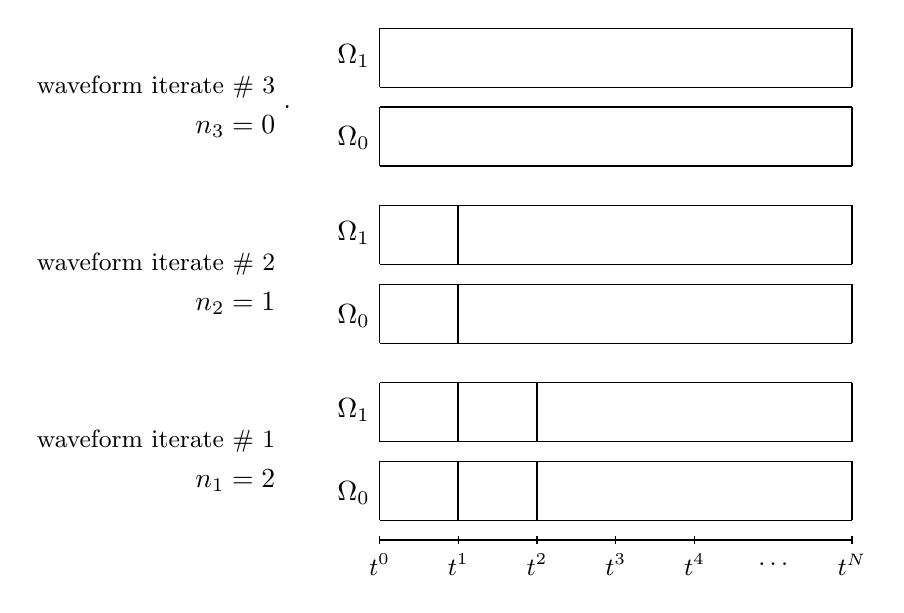
\begin{tikzpicture}[scale=1.0]

    \tikzstyle{dropline_style}=[densely dotted,thin]

    %\foreach \x/\xtext in {-1, -0.5/-\frac{1}{2}, 1}
    %\draw (\x cm,1pt) -- (\x cm,-1pt) node[anchor=north] {$\xtext$};

    \draw(-2,5) node[left] {.};
    \draw (-2.2, 0.75) node[left] {\small waveform iterate \# 1};
    \draw (-2.2, 3) node[left] {\small waveform iterate \# 2};
    \draw (-2.2, 5.25) node[left] {\small waveform iterate \# 3};

    \draw (-2.2, 0.25) node[left] {$n_1=2$};
    \draw (-2.2, 2.5) node[left] {$n_2=1$};
    \draw (-2.2, 4.75) node[left] {$n_3=0$};



    \def\a{-0.25}
    \def\b{0.5}
    \draw (-1,\a) -- (5,\a);
    \draw (5,\a) -- (5,\b);
    \draw (5,\b) -- (-1,\b);
    \draw (-1,\b) -- (-1,\a);

    \def\c{0.75}
    \def\d{1.5}
    \draw (-1,\c) -- (5,\c);
    \draw (5,\c) -- (5,\d);
    \draw (5,\d) -- (-1,\d);
    \draw (-1,\d) -- (-1,\c);

    \draw(-1,0.1) node[left] {$\Omega_0$};
    \draw(-1,1.15) node[left] {$\Omega_1$};

    \def\e{2}
    \def\f{2.75}
    \draw (-1,\e) -- (5,\e);
    \draw (5,\e) -- (5,\f);
    \draw (5,\f) -- (-1,\f);
    \draw (-1,\f) -- (-1,\e);

    \def\g{3}
    \def\h{3.75}
    \draw (-1,\g) -- (5,\g);
    \draw (5,\g) -- (5,\h);
    \draw (5,\h) -- (-1,\h);
    \draw (-1,\h) -- (-1,\g);

    \draw(-1,2.35) node[left] {$\Omega_0$};
    \draw(-1,3.4) node[left] {$\Omega_1$};

    \def\i{4.25}
    \def\j{5}
    \draw (-1,\i) -- (5,\i);
    \draw (5,\i) -- (5,\j);
    \draw (5,\j) -- (-1,\j);
    \draw (-1,\j) -- (-1,\i);

    \def\k{5.25}
    \def\l{6}
    \draw (-1,\k) -- (5,\k);
    \draw (5,\k) -- (5,\l);
    \draw (5,\l) -- (-1,\l);
    \draw (-1,\l) -- (-1,\k);

    \draw(-1,4.6) node[left] {$\Omega_0$};
    \draw(-1,5.65) node[left] {$\Omega_1$};


    % position of the time-line
    \def\y{-0.5}
    \draw [-] (-1,\y) -- (5,\y);

    \def\tick{0.05}
    \draw (-1,\y) ++(0,\tick) -- ++(0,-2*\tick) node[below] {\small $t^{0}$};
    \draw (0,\y) ++(0,\tick) -- ++(0,-2*\tick) node[below] {\small $t^{1}$};
    \draw (1,\y) ++(0,\tick) -- ++(0,-2*\tick) node[below] {\small $t^{2}$};
    \draw (2,\y) ++(0,\tick) -- ++(0,-2*\tick) node[below] {\small $t^{3}$};
    \draw (3,\y) ++(0,\tick) -- ++(0,-2*\tick) node[below] {\small $t^{4}$};
    \draw (4,\y)  node[below] {\small \phantom{t}$\ldots$\phantom{t}};  
    \draw (5,\y) ++(0,\tick) -- ++(0,-2*\tick) node[below] {\small $t^{N}$};
  
    % parameters for stencil diagrams
    \def\rad{0.12}
    \def\omr{0.88}   % 1-rad
    \def\intthick{0.068}   % thickness of integral bars

    %\draw [-latex,thick,blue] (0,0.2) -- (1,0.2);
    %\draw [-latex,thick,blue] (0,1.2) -- (1,1.2);

    %\draw [-latex,thick,blue] (-1,2.45) -- (0,2.45);
    %\draw [-latex,thick,blue] (-1,3.45) -- (0,3.45);

    \draw [-,thick,black] (0,\a) -- (0,\b);
    \draw [-,thick,black] (0,\c) -- (0,\d);

    \draw [-,thick,black] (1,\a) -- (1,\b);
    \draw [-,thick,black] (1,\c) -- (1,\d);

    \draw [-,thick,black] (0,\e) -- (0,\f);
    \draw [-,thick,black] (0,\g) -- (0,\h);

    %\draw (4,0.45)  node[below] {\small \phantom{t}$\ldots$\phantom{t}};  
    %\draw (4,1.45)  node[below] {\small \phantom{t}$\ldots$\phantom{t}};  
    
    % filled dots
    %% \foreach \xy in { (1,\b)}
    %% \filldraw [red] \xy circle (2pt);

    %% \foreach \xy in { (1,\c)}
    %% \filldraw [blue] \xy circle (2pt);

    %% \draw [->,thick,red] (1,0.5) arc (250:110:0.5 and 1.5);
    %% \draw [->,thick,blue] (1,0.75) arc (-70:70:0.5 and 0.8);

    %% \foreach \xy in { (0,\f)}
    %% \filldraw [red] \xy circle (2pt);

    %% \foreach \xy in { (0,\g)}
    %% \filldraw [blue] \xy circle (2pt);

    %% \draw [->,thick,red] (0,2.75) arc (250:110:0.5 and 1.5);
    %% \draw [->,thick,blue] (0,3) arc (-70:70:0.5 and 0.8);

  \end{tikzpicture}

  \end{figure}
  }   
  \only<11>{
  \begin{figure}
    \centering
    \definecolor{darkgreen}{rgb}{0,.6,0}
  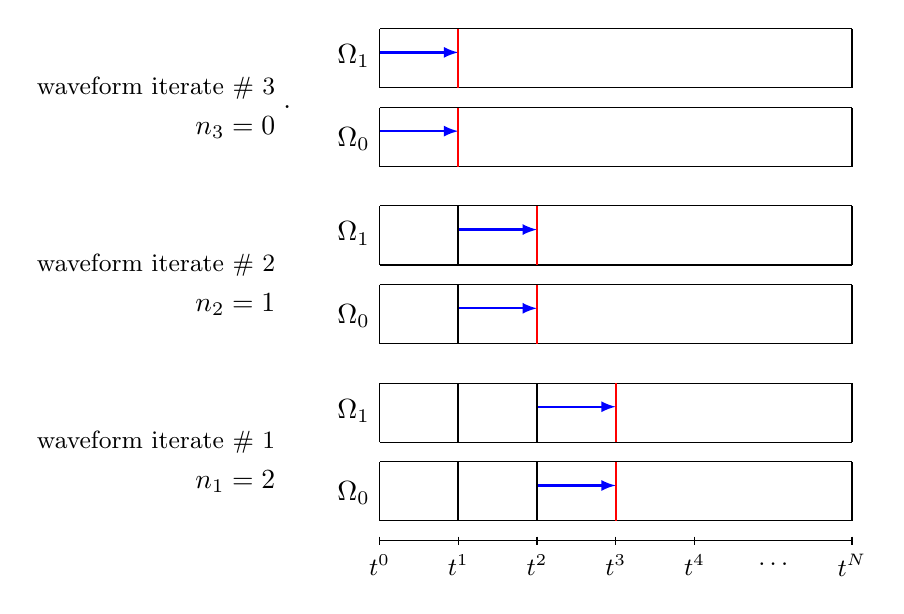
\begin{tikzpicture}[scale=1.0]

    \tikzstyle{dropline_style}=[densely dotted,thin]

    %\foreach \x/\xtext in {-1, -0.5/-\frac{1}{2}, 1}
    %\draw (\x cm,1pt) -- (\x cm,-1pt) node[anchor=north] {$\xtext$};

    \draw(-2,5) node[left] {.};
    \draw (-2.2, 0.75) node[left] {\small waveform iterate \# 1};
    \draw (-2.2, 3) node[left] {\small waveform iterate \# 2};
    \draw (-2.2, 5.25) node[left] {\small waveform iterate \# 3};

    \draw (-2.2, 0.25) node[left] {$n_1=2$};
    \draw (-2.2, 2.5) node[left] {$n_2=1$};
    \draw (-2.2, 4.75) node[left] {$n_3=0$};



    \def\a{-0.25}
    \def\b{0.5}
    \draw (-1,\a) -- (5,\a);
    \draw (5,\a) -- (5,\b);
    \draw (5,\b) -- (-1,\b);
    \draw (-1,\b) -- (-1,\a);

    \def\c{0.75}
    \def\d{1.5}
    \draw (-1,\c) -- (5,\c);
    \draw (5,\c) -- (5,\d);
    \draw (5,\d) -- (-1,\d);
    \draw (-1,\d) -- (-1,\c);

    \draw(-1,0.1) node[left] {$\Omega_0$};
    \draw(-1,1.15) node[left] {$\Omega_1$};

    \def\e{2}
    \def\f{2.75}
    \draw (-1,\e) -- (5,\e);
    \draw (5,\e) -- (5,\f);
    \draw (5,\f) -- (-1,\f);
    \draw (-1,\f) -- (-1,\e);

    \def\g{3}
    \def\h{3.75}
    \draw (-1,\g) -- (5,\g);
    \draw (5,\g) -- (5,\h);
    \draw (5,\h) -- (-1,\h);
    \draw (-1,\h) -- (-1,\g);

    \draw(-1,2.35) node[left] {$\Omega_0$};
    \draw(-1,3.4) node[left] {$\Omega_1$};

    \def\i{4.25}
    \def\j{5}
    \draw (-1,\i) -- (5,\i);
    \draw (5,\i) -- (5,\j);
    \draw (5,\j) -- (-1,\j);
    \draw (-1,\j) -- (-1,\i);

    \def\k{5.25}
    \def\l{6}
    \draw (-1,\k) -- (5,\k);
    \draw (5,\k) -- (5,\l);
    \draw (5,\l) -- (-1,\l);
    \draw (-1,\l) -- (-1,\k);

    \draw(-1,4.6) node[left] {$\Omega_0$};
    \draw(-1,5.65) node[left] {$\Omega_1$};


    % position of the time-line
    \def\y{-0.5}
    \draw [-] (-1,\y) -- (5,\y);

    \def\tick{0.05}
    \draw (-1,\y) ++(0,\tick) -- ++(0,-2*\tick) node[below] {\small $t^{0}$};
    \draw (0,\y) ++(0,\tick) -- ++(0,-2*\tick) node[below] {\small $t^{1}$};
    \draw (1,\y) ++(0,\tick) -- ++(0,-2*\tick) node[below] {\small $t^{2}$};
    \draw (2,\y) ++(0,\tick) -- ++(0,-2*\tick) node[below] {\small $t^{3}$};
    \draw (3,\y) ++(0,\tick) -- ++(0,-2*\tick) node[below] {\small $t^{4}$};
    \draw (4,\y)  node[below] {\small \phantom{t}$\ldots$\phantom{t}};  
    \draw (5,\y) ++(0,\tick) -- ++(0,-2*\tick) node[below] {\small $t^{N}$};
  
    % parameters for stencil diagrams
    \def\rad{0.12}
    \def\omr{0.88}   % 1-rad
    \def\intthick{0.068}   % thickness of integral bars

    \draw [-latex,thick,blue] (1,0.2) -- (2,0.2);
    \draw [-latex,thick,blue] (1,1.2) -- (2,1.2);

    \draw [-latex,thick,blue] (0,2.45) -- (1,2.45);
    \draw [-latex,thick,blue] (0,3.45) -- (1,3.45);

    \draw [-latex,thick,blue] (-1,4.7) -- (0,4.7);
    \draw [-latex,thick,blue] (-1,5.7) -- (0,5.7);

    \draw [-,thick,black] (0,\a) -- (0,\b);
    \draw [-,thick,black] (0,\c) -- (0,\d);

    \draw [-,thick,black] (1,\a) -- (1,\b);
    \draw [-,thick,black] (1,\c) -- (1,\d);

    \draw [-,thick,black] (0,\e) -- (0,\f);
    \draw [-,thick,black] (0,\g) -- (0,\h);

    \draw [-,thick,red] (2,\a) -- (2,\b);
    \draw [-,thick,red] (2,\c) -- (2,\d);

    \draw [-,thick,red] (1,\e) -- (1,\f);
    \draw [-,thick,red] (1,\g) -- (1,\h);

    \draw [-,thick,red] (0,\i) -- (0,\j);
    \draw [-,thick,red] (0,\k) -- (0,\l);


    %\draw (4,0.45)  node[below] {\small \phantom{t}$\ldots$\phantom{t}};  
    %\draw (4,1.45)  node[below] {\small \phantom{t}$\ldots$\phantom{t}};  
    
    % filled dots
    %% \foreach \xy in { (1,\b)}
    %% \filldraw [red] \xy circle (2pt);

    %% \foreach \xy in { (1,\c)}
    %% \filldraw [blue] \xy circle (2pt);

    %% \draw [->,thick,red] (1,0.5) arc (250:110:0.5 and 1.5);
    %% \draw [->,thick,blue] (1,0.75) arc (-70:70:0.5 and 0.8);

    %% \foreach \xy in { (0,\f)}
    %% \filldraw [red] \xy circle (2pt);

    %% \foreach \xy in { (0,\g)}
    %% \filldraw [blue] \xy circle (2pt);

    %% \draw [->,thick,red] (0,2.75) arc (250:110:0.5 and 1.5);
    %% \draw [->,thick,blue] (0,3) arc (-70:70:0.5 and 0.8);

  \end{tikzpicture}

  \end{figure}
  }    
  \only<12>{
  \begin{figure}
    \centering
    \definecolor{darkgreen}{rgb}{0,.6,0}
  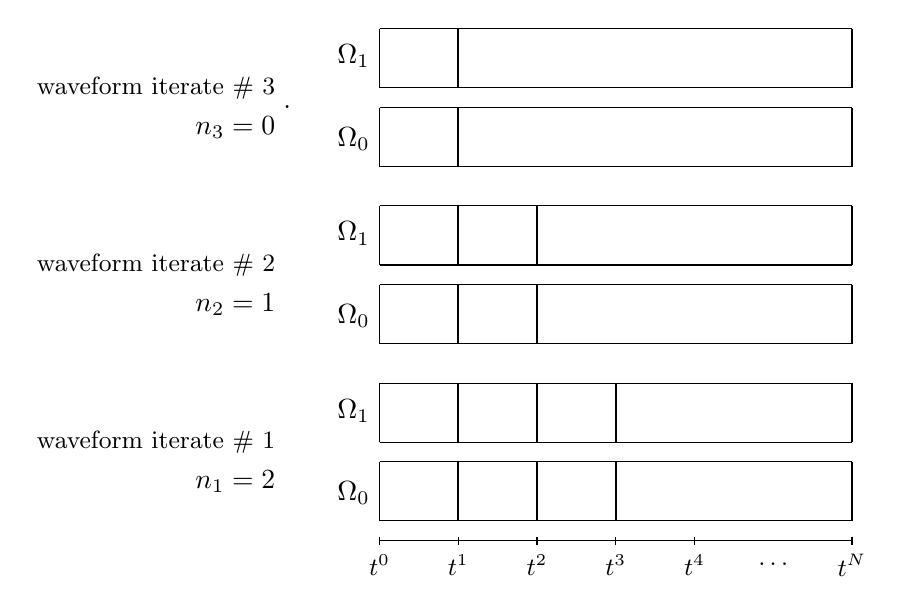
\begin{tikzpicture}[scale=1.0]

    \tikzstyle{dropline_style}=[densely dotted,thin]

    %\foreach \x/\xtext in {-1, -0.5/-\frac{1}{2}, 1}
    %\draw (\x cm,1pt) -- (\x cm,-1pt) node[anchor=north] {$\xtext$};

    \draw(-2,5) node[left] {.};
    \draw (-2.2, 0.75) node[left] {\small waveform iterate \# 1};
    \draw (-2.2, 3) node[left] {\small waveform iterate \# 2};
    \draw (-2.2, 5.25) node[left] {\small waveform iterate \# 3};

    \draw (-2.2, 0.25) node[left] {$n_1=2$};
    \draw (-2.2, 2.5) node[left] {$n_2=1$};
    \draw (-2.2, 4.75) node[left] {$n_3=0$};



    \def\a{-0.25}
    \def\b{0.5}
    \draw (-1,\a) -- (5,\a);
    \draw (5,\a) -- (5,\b);
    \draw (5,\b) -- (-1,\b);
    \draw (-1,\b) -- (-1,\a);

    \def\c{0.75}
    \def\d{1.5}
    \draw (-1,\c) -- (5,\c);
    \draw (5,\c) -- (5,\d);
    \draw (5,\d) -- (-1,\d);
    \draw (-1,\d) -- (-1,\c);

    \draw(-1,0.1) node[left] {$\Omega_0$};
    \draw(-1,1.15) node[left] {$\Omega_1$};

    \def\e{2}
    \def\f{2.75}
    \draw (-1,\e) -- (5,\e);
    \draw (5,\e) -- (5,\f);
    \draw (5,\f) -- (-1,\f);
    \draw (-1,\f) -- (-1,\e);

    \def\g{3}
    \def\h{3.75}
    \draw (-1,\g) -- (5,\g);
    \draw (5,\g) -- (5,\h);
    \draw (5,\h) -- (-1,\h);
    \draw (-1,\h) -- (-1,\g);

    \draw(-1,2.35) node[left] {$\Omega_0$};
    \draw(-1,3.4) node[left] {$\Omega_1$};

    \def\i{4.25}
    \def\j{5}
    \draw (-1,\i) -- (5,\i);
    \draw (5,\i) -- (5,\j);
    \draw (5,\j) -- (-1,\j);
    \draw (-1,\j) -- (-1,\i);

    \def\k{5.25}
    \def\l{6}
    \draw (-1,\k) -- (5,\k);
    \draw (5,\k) -- (5,\l);
    \draw (5,\l) -- (-1,\l);
    \draw (-1,\l) -- (-1,\k);

    \draw(-1,4.6) node[left] {$\Omega_0$};
    \draw(-1,5.65) node[left] {$\Omega_1$};


    % position of the time-line
    \def\y{-0.5}
    \draw [-] (-1,\y) -- (5,\y);

    \def\tick{0.05}
    \draw (-1,\y) ++(0,\tick) -- ++(0,-2*\tick) node[below] {\small $t^{0}$};
    \draw (0,\y) ++(0,\tick) -- ++(0,-2*\tick) node[below] {\small $t^{1}$};
    \draw (1,\y) ++(0,\tick) -- ++(0,-2*\tick) node[below] {\small $t^{2}$};
    \draw (2,\y) ++(0,\tick) -- ++(0,-2*\tick) node[below] {\small $t^{3}$};
    \draw (3,\y) ++(0,\tick) -- ++(0,-2*\tick) node[below] {\small $t^{4}$};
    \draw (4,\y)  node[below] {\small \phantom{t}$\ldots$\phantom{t}};  
    \draw (5,\y) ++(0,\tick) -- ++(0,-2*\tick) node[below] {\small $t^{N}$};
  
    % parameters for stencil diagrams
    \def\rad{0.12}
    \def\omr{0.88}   % 1-rad
    \def\intthick{0.068}   % thickness of integral bars

    %% \draw [-latex,thick,blue] (1,0.2) -- (2,0.2);
    %% \draw [-latex,thick,blue] (1,1.2) -- (2,1.2);

    %% \draw [-latex,thick,blue] (0,2.45) -- (1,2.45);
    %% \draw [-latex,thick,blue] (0,3.45) -- (1,3.45);

    %% \draw [-latex,thick,blue] (-1,4.7) -- (0,4.7);
    %% \draw [-latex,thick,blue] (-1,5.7) -- (0,5.7);

    \draw [-,thick,black] (0,\a) -- (0,\b);
    \draw [-,thick,black] (0,\c) -- (0,\d);

    \draw [-,thick,black] (1,\a) -- (1,\b);
    \draw [-,thick,black] (1,\c) -- (1,\d);

    \draw [-,thick,black] (0,\e) -- (0,\f);
    \draw [-,thick,black] (0,\g) -- (0,\h);

    \draw [-,thick,black] (2,\a) -- (2,\b);
    \draw [-,thick,black] (2,\c) -- (2,\d);

    \draw [-,thick,black] (1,\e) -- (1,\f);
    \draw [-,thick,black] (1,\g) -- (1,\h);

    \draw [-,thick,black] (0,\i) -- (0,\j);
    \draw [-,thick,black] (0,\k) -- (0,\l);


    %\draw (4,0.45)  node[below] {\small \phantom{t}$\ldots$\phantom{t}};  
    %\draw (4,1.45)  node[below] {\small \phantom{t}$\ldots$\phantom{t}};  
    
    % filled dots
    %% \foreach \xy in { (1,\b)}
    %% \filldraw [red] \xy circle (2pt);

    %% \foreach \xy in { (1,\c)}
    %% \filldraw [blue] \xy circle (2pt);

    %% \draw [->,thick,red] (1,0.5) arc (250:110:0.5 and 1.5);
    %% \draw [->,thick,blue] (1,0.75) arc (-70:70:0.5 and 0.8);

    %% \foreach \xy in { (0,\f)}
    %% \filldraw [red] \xy circle (2pt);

    %% \foreach \xy in { (0,\g)}
    %% \filldraw [blue] \xy circle (2pt);

    %% \draw [->,thick,red] (0,2.75) arc (250:110:0.5 and 1.5);
    %% \draw [->,thick,blue] (0,3) arc (-70:70:0.5 and 0.8);

  \end{tikzpicture}

  \end{figure}
  }    
  \only<13>{
  \begin{figure}
    \centering
    \definecolor{darkgreen}{rgb}{0,.6,0}
  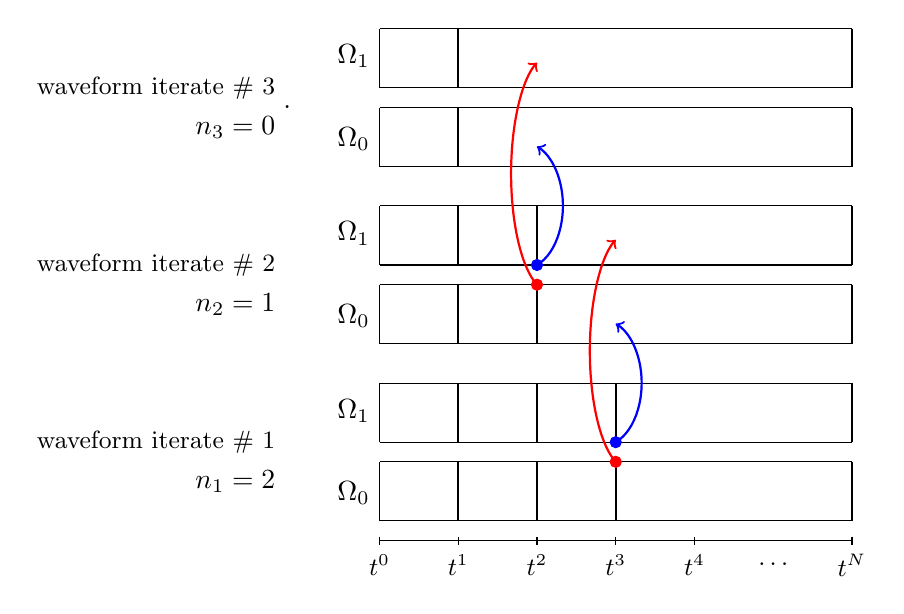
\begin{tikzpicture}[scale=1.0]

    \tikzstyle{dropline_style}=[densely dotted,thin]

    %\foreach \x/\xtext in {-1, -0.5/-\frac{1}{2}, 1}
    %\draw (\x cm,1pt) -- (\x cm,-1pt) node[anchor=north] {$\xtext$};

    \draw(-2,5) node[left] {.};
    \draw (-2.2, 0.75) node[left] {\small waveform iterate \# 1};
    \draw (-2.2, 3) node[left] {\small waveform iterate \# 2};
    \draw (-2.2, 5.25) node[left] {\small waveform iterate \# 3};

    \draw (-2.2, 0.25) node[left] {$n_1=2$};
    \draw (-2.2, 2.5) node[left] {$n_2=1$};
    \draw (-2.2, 4.75) node[left] {$n_3=0$};



    \def\a{-0.25}
    \def\b{0.5}
    \draw (-1,\a) -- (5,\a);
    \draw (5,\a) -- (5,\b);
    \draw (5,\b) -- (-1,\b);
    \draw (-1,\b) -- (-1,\a);

    \def\c{0.75}
    \def\d{1.5}
    \draw (-1,\c) -- (5,\c);
    \draw (5,\c) -- (5,\d);
    \draw (5,\d) -- (-1,\d);
    \draw (-1,\d) -- (-1,\c);

    \draw(-1,0.1) node[left] {$\Omega_0$};
    \draw(-1,1.15) node[left] {$\Omega_1$};

    \def\e{2}
    \def\f{2.75}
    \draw (-1,\e) -- (5,\e);
    \draw (5,\e) -- (5,\f);
    \draw (5,\f) -- (-1,\f);
    \draw (-1,\f) -- (-1,\e);

    \def\g{3}
    \def\h{3.75}
    \draw (-1,\g) -- (5,\g);
    \draw (5,\g) -- (5,\h);
    \draw (5,\h) -- (-1,\h);
    \draw (-1,\h) -- (-1,\g);

    \draw(-1,2.35) node[left] {$\Omega_0$};
    \draw(-1,3.4) node[left] {$\Omega_1$};

    \def\i{4.25}
    \def\j{5}
    \draw (-1,\i) -- (5,\i);
    \draw (5,\i) -- (5,\j);
    \draw (5,\j) -- (-1,\j);
    \draw (-1,\j) -- (-1,\i);

    \def\k{5.25}
    \def\l{6}
    \draw (-1,\k) -- (5,\k);
    \draw (5,\k) -- (5,\l);
    \draw (5,\l) -- (-1,\l);
    \draw (-1,\l) -- (-1,\k);

    \draw(-1,4.6) node[left] {$\Omega_0$};
    \draw(-1,5.65) node[left] {$\Omega_1$};


    % position of the time-line
    \def\y{-0.5}
    \draw [-] (-1,\y) -- (5,\y);

    \def\tick{0.05}
    \draw (-1,\y) ++(0,\tick) -- ++(0,-2*\tick) node[below] {\small $t^{0}$};
    \draw (0,\y) ++(0,\tick) -- ++(0,-2*\tick) node[below] {\small $t^{1}$};
    \draw (1,\y) ++(0,\tick) -- ++(0,-2*\tick) node[below] {\small $t^{2}$};
    \draw (2,\y) ++(0,\tick) -- ++(0,-2*\tick) node[below] {\small $t^{3}$};
    \draw (3,\y) ++(0,\tick) -- ++(0,-2*\tick) node[below] {\small $t^{4}$};
    \draw (4,\y)  node[below] {\small \phantom{t}$\ldots$\phantom{t}};  
    \draw (5,\y) ++(0,\tick) -- ++(0,-2*\tick) node[below] {\small $t^{N}$};
  
    % parameters for stencil diagrams
    \def\rad{0.12}
    \def\omr{0.88}   % 1-rad
    \def\intthick{0.068}   % thickness of integral bars

    %% \draw [-latex,thick,blue] (1,0.2) -- (2,0.2);
    %% \draw [-latex,thick,blue] (1,1.2) -- (2,1.2);

    %% \draw [-latex,thick,blue] (0,2.45) -- (1,2.45);
    %% \draw [-latex,thick,blue] (0,3.45) -- (1,3.45);

    %% \draw [-latex,thick,blue] (-1,4.7) -- (0,4.7);
    %% \draw [-latex,thick,blue] (-1,5.7) -- (0,5.7);

    \draw [-,thick,black] (0,\a) -- (0,\b);
    \draw [-,thick,black] (0,\c) -- (0,\d);

    \draw [-,thick,black] (1,\a) -- (1,\b);
    \draw [-,thick,black] (1,\c) -- (1,\d);

    \draw [-,thick,black] (0,\e) -- (0,\f);
    \draw [-,thick,black] (0,\g) -- (0,\h);

    \draw [-,thick,black] (2,\a) -- (2,\b);
    \draw [-,thick,black] (2,\c) -- (2,\d);

    \draw [-,thick,black] (1,\e) -- (1,\f);
    \draw [-,thick,black] (1,\g) -- (1,\h);

    \draw [-,thick,black] (0,\i) -- (0,\j);
    \draw [-,thick,black] (0,\k) -- (0,\l);


    %\draw (4,0.45)  node[below] {\small \phantom{t}$\ldots$\phantom{t}};  
    %\draw (4,1.45)  node[below] {\small \phantom{t}$\ldots$\phantom{t}};  
    
    % filled dots
    \foreach \xy in { (2,\b)}
    \filldraw [red] \xy circle (2pt);

    \foreach \xy in { (2,\c)}
    \filldraw [blue] \xy circle (2pt);

    \draw [->,thick,red] (2,0.5) arc (250:110:0.5 and 1.5);
    \draw [->,thick,blue] (2,0.75) arc (-70:70:0.5 and 0.8);

    \foreach \xy in { (1,\f)}
    \filldraw [red] \xy circle (2pt);

    \foreach \xy in { (1,\g)}
    \filldraw [blue] \xy circle (2pt);

    \draw [->,thick,red] (1,2.75) arc (250:110:0.5 and 1.5);
    \draw [->,thick,blue] (1,3) arc (-70:70:0.5 and 0.8);

  \end{tikzpicture}

  \end{figure}
  }   
  \only<14>{
  \begin{figure}
    \centering
    \definecolor{darkgreen}{rgb}{0,.6,0}
  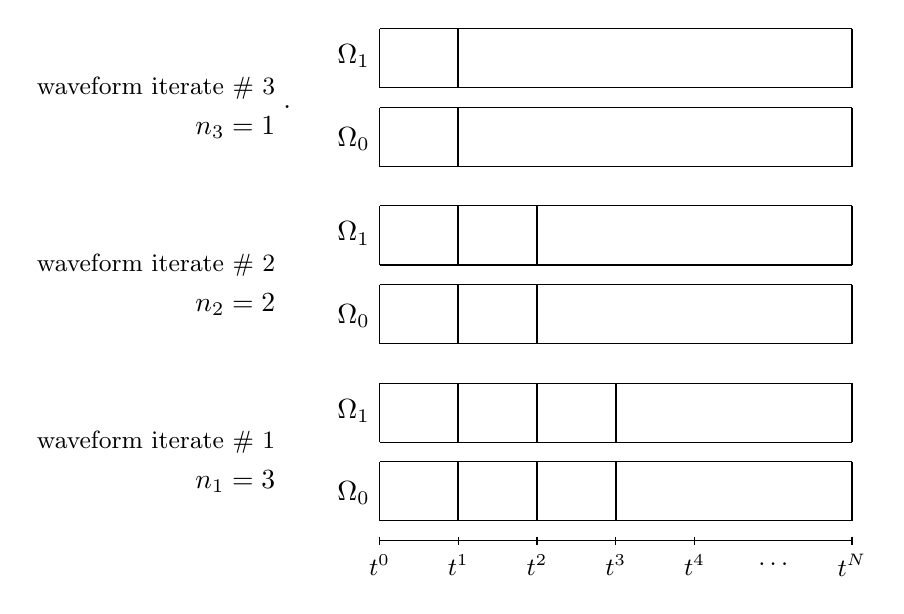
\begin{tikzpicture}[scale=1.0]

    \tikzstyle{dropline_style}=[densely dotted,thin]

    %\foreach \x/\xtext in {-1, -0.5/-\frac{1}{2}, 1}
    %\draw (\x cm,1pt) -- (\x cm,-1pt) node[anchor=north] {$\xtext$};

    \draw(-2,5) node[left] {.};
    \draw (-2.2, 0.75) node[left] {\small waveform iterate \# 1};
    \draw (-2.2, 3) node[left] {\small waveform iterate \# 2};
    \draw (-2.2, 5.25) node[left] {\small waveform iterate \# 3};

    \draw (-2.2, 0.25) node[left] {$n_1=3$};
    \draw (-2.2, 2.5) node[left] {$n_2=2$};
    \draw (-2.2, 4.75) node[left] {$n_3=1$};



    \def\a{-0.25}
    \def\b{0.5}
    \draw (-1,\a) -- (5,\a);
    \draw (5,\a) -- (5,\b);
    \draw (5,\b) -- (-1,\b);
    \draw (-1,\b) -- (-1,\a);

    \def\c{0.75}
    \def\d{1.5}
    \draw (-1,\c) -- (5,\c);
    \draw (5,\c) -- (5,\d);
    \draw (5,\d) -- (-1,\d);
    \draw (-1,\d) -- (-1,\c);

    \draw(-1,0.1) node[left] {$\Omega_0$};
    \draw(-1,1.15) node[left] {$\Omega_1$};

    \def\e{2}
    \def\f{2.75}
    \draw (-1,\e) -- (5,\e);
    \draw (5,\e) -- (5,\f);
    \draw (5,\f) -- (-1,\f);
    \draw (-1,\f) -- (-1,\e);

    \def\g{3}
    \def\h{3.75}
    \draw (-1,\g) -- (5,\g);
    \draw (5,\g) -- (5,\h);
    \draw (5,\h) -- (-1,\h);
    \draw (-1,\h) -- (-1,\g);

    \draw(-1,2.35) node[left] {$\Omega_0$};
    \draw(-1,3.4) node[left] {$\Omega_1$};

    \def\i{4.25}
    \def\j{5}
    \draw (-1,\i) -- (5,\i);
    \draw (5,\i) -- (5,\j);
    \draw (5,\j) -- (-1,\j);
    \draw (-1,\j) -- (-1,\i);

    \def\k{5.25}
    \def\l{6}
    \draw (-1,\k) -- (5,\k);
    \draw (5,\k) -- (5,\l);
    \draw (5,\l) -- (-1,\l);
    \draw (-1,\l) -- (-1,\k);

    \draw(-1,4.6) node[left] {$\Omega_0$};
    \draw(-1,5.65) node[left] {$\Omega_1$};


    % position of the time-line
    \def\y{-0.5}
    \draw [-] (-1,\y) -- (5,\y);

    \def\tick{0.05}
    \draw (-1,\y) ++(0,\tick) -- ++(0,-2*\tick) node[below] {\small $t^{0}$};
    \draw (0,\y) ++(0,\tick) -- ++(0,-2*\tick) node[below] {\small $t^{1}$};
    \draw (1,\y) ++(0,\tick) -- ++(0,-2*\tick) node[below] {\small $t^{2}$};
    \draw (2,\y) ++(0,\tick) -- ++(0,-2*\tick) node[below] {\small $t^{3}$};
    \draw (3,\y) ++(0,\tick) -- ++(0,-2*\tick) node[below] {\small $t^{4}$};
    \draw (4,\y)  node[below] {\small \phantom{t}$\ldots$\phantom{t}};  
    \draw (5,\y) ++(0,\tick) -- ++(0,-2*\tick) node[below] {\small $t^{N}$};
  
    % parameters for stencil diagrams
    \def\rad{0.12}
    \def\omr{0.88}   % 1-rad
    \def\intthick{0.068}   % thickness of integral bars

    %% \draw [-latex,thick,blue] (1,0.2) -- (2,0.2);
    %% \draw [-latex,thick,blue] (1,1.2) -- (2,1.2);

    %% \draw [-latex,thick,blue] (0,2.45) -- (1,2.45);
    %% \draw [-latex,thick,blue] (0,3.45) -- (1,3.45);

    %% \draw [-latex,thick,blue] (-1,4.7) -- (0,4.7);
    %% \draw [-latex,thick,blue] (-1,5.7) -- (0,5.7);

    \draw [-,thick,black] (0,\a) -- (0,\b);
    \draw [-,thick,black] (0,\c) -- (0,\d);

    \draw [-,thick,black] (1,\a) -- (1,\b);
    \draw [-,thick,black] (1,\c) -- (1,\d);

    \draw [-,thick,black] (0,\e) -- (0,\f);
    \draw [-,thick,black] (0,\g) -- (0,\h);

    \draw [-,thick,black] (2,\a) -- (2,\b);
    \draw [-,thick,black] (2,\c) -- (2,\d);

    \draw [-,thick,black] (1,\e) -- (1,\f);
    \draw [-,thick,black] (1,\g) -- (1,\h);

    \draw [-,thick,black] (0,\i) -- (0,\j);
    \draw [-,thick,black] (0,\k) -- (0,\l);


    %\draw (4,0.45)  node[below] {\small \phantom{t}$\ldots$\phantom{t}};  
    %\draw (4,1.45)  node[below] {\small \phantom{t}$\ldots$\phantom{t}};  
    
    % filled dots
    %% \foreach \xy in { (2,\b)}
    %% \filldraw [red] \xy circle (2pt);

    %% \foreach \xy in { (2,\c)}
    %% \filldraw [blue] \xy circle (2pt);

    %% \draw [->,thick,red] (2,0.5) arc (250:110:0.5 and 1.5);
    %% \draw [->,thick,blue] (2,0.75) arc (-70:70:0.5 and 0.8);

    %% \foreach \xy in { (1,\f)}
    %% \filldraw [red] \xy circle (2pt);

    %% \foreach \xy in { (1,\g)}
    %% \filldraw [blue] \xy circle (2pt);

    %% \draw [->,thick,red] (1,2.75) arc (250:110:0.5 and 1.5);
    %% \draw [->,thick,blue] (1,3) arc (-70:70:0.5 and 0.8);

  \end{tikzpicture}

  \end{figure}
  }  
  \only<15>{
  \begin{figure}
    \centering
    \definecolor{darkgreen}{rgb}{0,.6,0}
  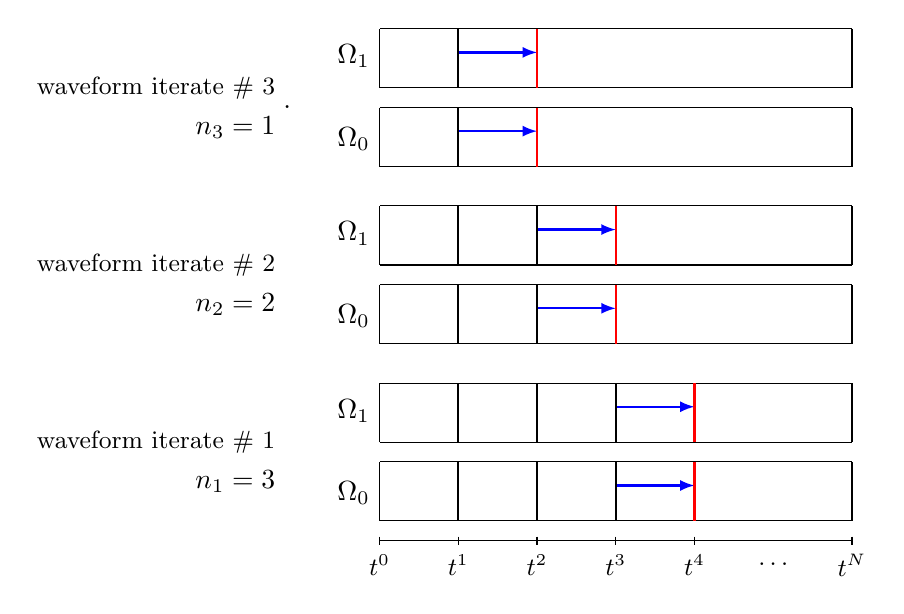
\begin{tikzpicture}[scale=1.0]

    \tikzstyle{dropline_style}=[densely dotted,thin]

    %\foreach \x/\xtext in {-1, -0.5/-\frac{1}{2}, 1}
    %\draw (\x cm,1pt) -- (\x cm,-1pt) node[anchor=north] {$\xtext$};

    \draw(-2,5) node[left] {.};
    \draw (-2.2, 0.75) node[left] {\small waveform iterate \# 1};
    \draw (-2.2, 3) node[left] {\small waveform iterate \# 2};
    \draw (-2.2, 5.25) node[left] {\small waveform iterate \# 3};

    \draw (-2.2, 0.25) node[left] {$n_1=3$};
    \draw (-2.2, 2.5) node[left] {$n_2=2$};
    \draw (-2.2, 4.75) node[left] {$n_3=1$};



    \def\a{-0.25}
    \def\b{0.5}
    \draw (-1,\a) -- (5,\a);
    \draw (5,\a) -- (5,\b);
    \draw (5,\b) -- (-1,\b);
    \draw (-1,\b) -- (-1,\a);

    \def\c{0.75}
    \def\d{1.5}
    \draw (-1,\c) -- (5,\c);
    \draw (5,\c) -- (5,\d);
    \draw (5,\d) -- (-1,\d);
    \draw (-1,\d) -- (-1,\c);

    \draw(-1,0.1) node[left] {$\Omega_0$};
    \draw(-1,1.15) node[left] {$\Omega_1$};

    \def\e{2}
    \def\f{2.75}
    \draw (-1,\e) -- (5,\e);
    \draw (5,\e) -- (5,\f);
    \draw (5,\f) -- (-1,\f);
    \draw (-1,\f) -- (-1,\e);

    \def\g{3}
    \def\h{3.75}
    \draw (-1,\g) -- (5,\g);
    \draw (5,\g) -- (5,\h);
    \draw (5,\h) -- (-1,\h);
    \draw (-1,\h) -- (-1,\g);

    \draw(-1,2.35) node[left] {$\Omega_0$};
    \draw(-1,3.4) node[left] {$\Omega_1$};

    \def\i{4.25}
    \def\j{5}
    \draw (-1,\i) -- (5,\i);
    \draw (5,\i) -- (5,\j);
    \draw (5,\j) -- (-1,\j);
    \draw (-1,\j) -- (-1,\i);

    \def\k{5.25}
    \def\l{6}
    \draw (-1,\k) -- (5,\k);
    \draw (5,\k) -- (5,\l);
    \draw (5,\l) -- (-1,\l);
    \draw (-1,\l) -- (-1,\k);

    \draw(-1,4.6) node[left] {$\Omega_0$};
    \draw(-1,5.65) node[left] {$\Omega_1$};


    % position of the time-line
    \def\y{-0.5}
    \draw [-] (-1,\y) -- (5,\y);

    \def\tick{0.05}
    \draw (-1,\y) ++(0,\tick) -- ++(0,-2*\tick) node[below] {\small $t^{0}$};
    \draw (0,\y) ++(0,\tick) -- ++(0,-2*\tick) node[below] {\small $t^{1}$};
    \draw (1,\y) ++(0,\tick) -- ++(0,-2*\tick) node[below] {\small $t^{2}$};
    \draw (2,\y) ++(0,\tick) -- ++(0,-2*\tick) node[below] {\small $t^{3}$};
    \draw (3,\y) ++(0,\tick) -- ++(0,-2*\tick) node[below] {\small $t^{4}$};
    \draw (4,\y)  node[below] {\small \phantom{t}$\ldots$\phantom{t}};  
    \draw (5,\y) ++(0,\tick) -- ++(0,-2*\tick) node[below] {\small $t^{N}$};
  
    % parameters for stencil diagrams
    \def\rad{0.12}
    \def\omr{0.88}   % 1-rad
    \def\intthick{0.068}   % thickness of integral bars

    \draw [-latex,thick,blue] (2,0.2) -- (3,0.2);
    \draw [-latex,thick,blue] (2,1.2) -- (3,1.2);

    \draw [-latex,thick,blue] (1,2.45) -- (2,2.45);
    \draw [-latex,thick,blue] (1,3.45) -- (2,3.45);

    \draw [-latex,thick,blue] (0,4.7) -- (1,4.7);
    \draw [-latex,thick,blue] (0,5.7) -- (1,5.7);

    \draw [-,thick,black] (0,\a) -- (0,\b);
    \draw [-,thick,black] (0,\c) -- (0,\d);

    \draw [-,thick,black] (1,\a) -- (1,\b);
    \draw [-,thick,black] (1,\c) -- (1,\d);

    \draw [-,thick,black] (0,\e) -- (0,\f);
    \draw [-,thick,black] (0,\g) -- (0,\h);

    \draw [-,thick,black] (2,\a) -- (2,\b);
    \draw [-,thick,black] (2,\c) -- (2,\d);

    \draw [-,thick,black] (1,\e) -- (1,\f);
    \draw [-,thick,black] (1,\g) -- (1,\h);

    \draw [-,thick,black] (0,\i) -- (0,\j);
    \draw [-,thick,black] (0,\k) -- (0,\l);

    \draw [-,thick,red] (3,\a) -- (3,\b);
    \draw [-,thick,red] (3,\c) -- (3,\d);

    \draw [-,thick,red] (2,\e) -- (2,\f);
    \draw [-,thick,red] (2,\g) -- (2,\h);

    \draw [-,thick,red] (1,\i) -- (1,\j);
    \draw [-,thick,red] (1,\k) -- (1,\l);

    %\draw (4,0.45)  node[below] {\small \phantom{t}$\ldots$\phantom{t}};  
    %\draw (4,1.45)  node[below] {\small \phantom{t}$\ldots$\phantom{t}};  
    
    % filled dots
    %% \foreach \xy in { (2,\b)}
    %% \filldraw [red] \xy circle (2pt);

    %% \foreach \xy in { (2,\c)}
    %% \filldraw [blue] \xy circle (2pt);

    %% \draw [->,thick,red] (2,0.5) arc (250:110:0.5 and 1.5);
    %% \draw [->,thick,blue] (2,0.75) arc (-70:70:0.5 and 0.8);

    %% \foreach \xy in { (1,\f)}
    %% \filldraw [red] \xy circle (2pt);

    %% \foreach \xy in { (1,\g)}
    %% \filldraw [blue] \xy circle (2pt);

    %% \draw [->,thick,red] (1,2.75) arc (250:110:0.5 and 1.5);
    %% \draw [->,thick,blue] (1,3) arc (-70:70:0.5 and 0.8);

  \end{tikzpicture}

  \end{figure}
  }  
\end{frame}

\begin{frame}
  % Intuitive figure
  \frametitle{Pipeline Schwarz Waveform Relaxation}
  \centering
  \includegraphics[height=0.7\textheight]{figures/pswr}
\end{frame}


\section{Implementation}

\begin{frame}{Charm}

  \begin{itemize}
  \item Each Chare represents one iteration on one domain
  \item Chares communicate with their neighbors on adjacent domains
    in the next iteration
  \item Currently all communication is done with marshaled parameters
  \end{itemize}

  % Intuitive figure
  \frametitle{Pipeline Schwarz Waveform Relaxation}
  \centering
  \includegraphics[height=0.5\textheight]{figures/pswr}

\end{frame}

\begin{frame}{Local Time Adaptivity}

  \begin{columns}

    \begin{column}{.4\textwidth}

      \begin{itemize}
      \item $dt$ changes within predefined ``chunks''
      \item Natural extension to PSWR
      \end{itemize}
      
    \end{column}

    \begin{column}{.6\textwidth}

      \begin{figure}
        \centering
        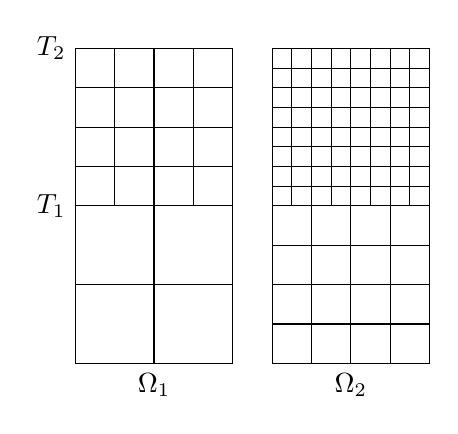
\begin{tikzpicture}
          % \draw[<-] (-.5,4) -- (-.5,0) node[pos=.1,left] {t};
          \draw (0,0) grid (2,2);
          \draw[step=.5] (0,2) grid (2,4);
          \draw (0,2) node[left] {$T_1$};
          \draw (0,4) node[left] {$T_2$};
          \draw (1,0) node[below] {$\Omega_1$};
          \draw[step=.5] (2.499,0) grid (4.5,2);
          \draw[step=.25] (2.499,2) grid (4.5,4);
          \draw (3.5,0) node[below] {$\Omega_2$};
        \end{tikzpicture}
      \end{figure}

    \end{column}
  \end{columns}

\end{frame}

\begin{frame}{LiveVis}
  
\end{frame}

\section{Numerical Experiments}

\begin{frame}{Numerical Experiments}{DummyLB, GreedyLB, RefineLB}
  
  \begin{itemize}
  \item Solving 2D diffusion equation on $\Omega = [0,2\pi]^2$ using a
    uniform mesh with $N_x = N_y = 1600$, $2.56M$ unknowns
  \item Subdomain solutions are calculated with a BTCS finite
    difference stencil using sparse matrix routines in PETSc
  \item 16 subdomains $\Omega_{i,j}$ ($1\leq i,j \leq 4$) with an
    overlap of 20
  \item 10 time steps for $i\geq3$, 20 time steps for $i\leq2$
  \item Load balance every 5 iterations for a total of 40 iterations
  \item 2 nodes, 4 cores/node
  \end{itemize}
\end{frame}

\begin{frame}{Numerical Experiments}{DummyLB}
  \begin{figure}
%    \floatbox[{\capbeside\thisfloatsetup{capbesideposition={left,top}}}]{figure}[\FBwidth]
%    {\caption{Time Profile}\label{fig:test}}
%    {\includegraphics[width=5cm]{name}}
    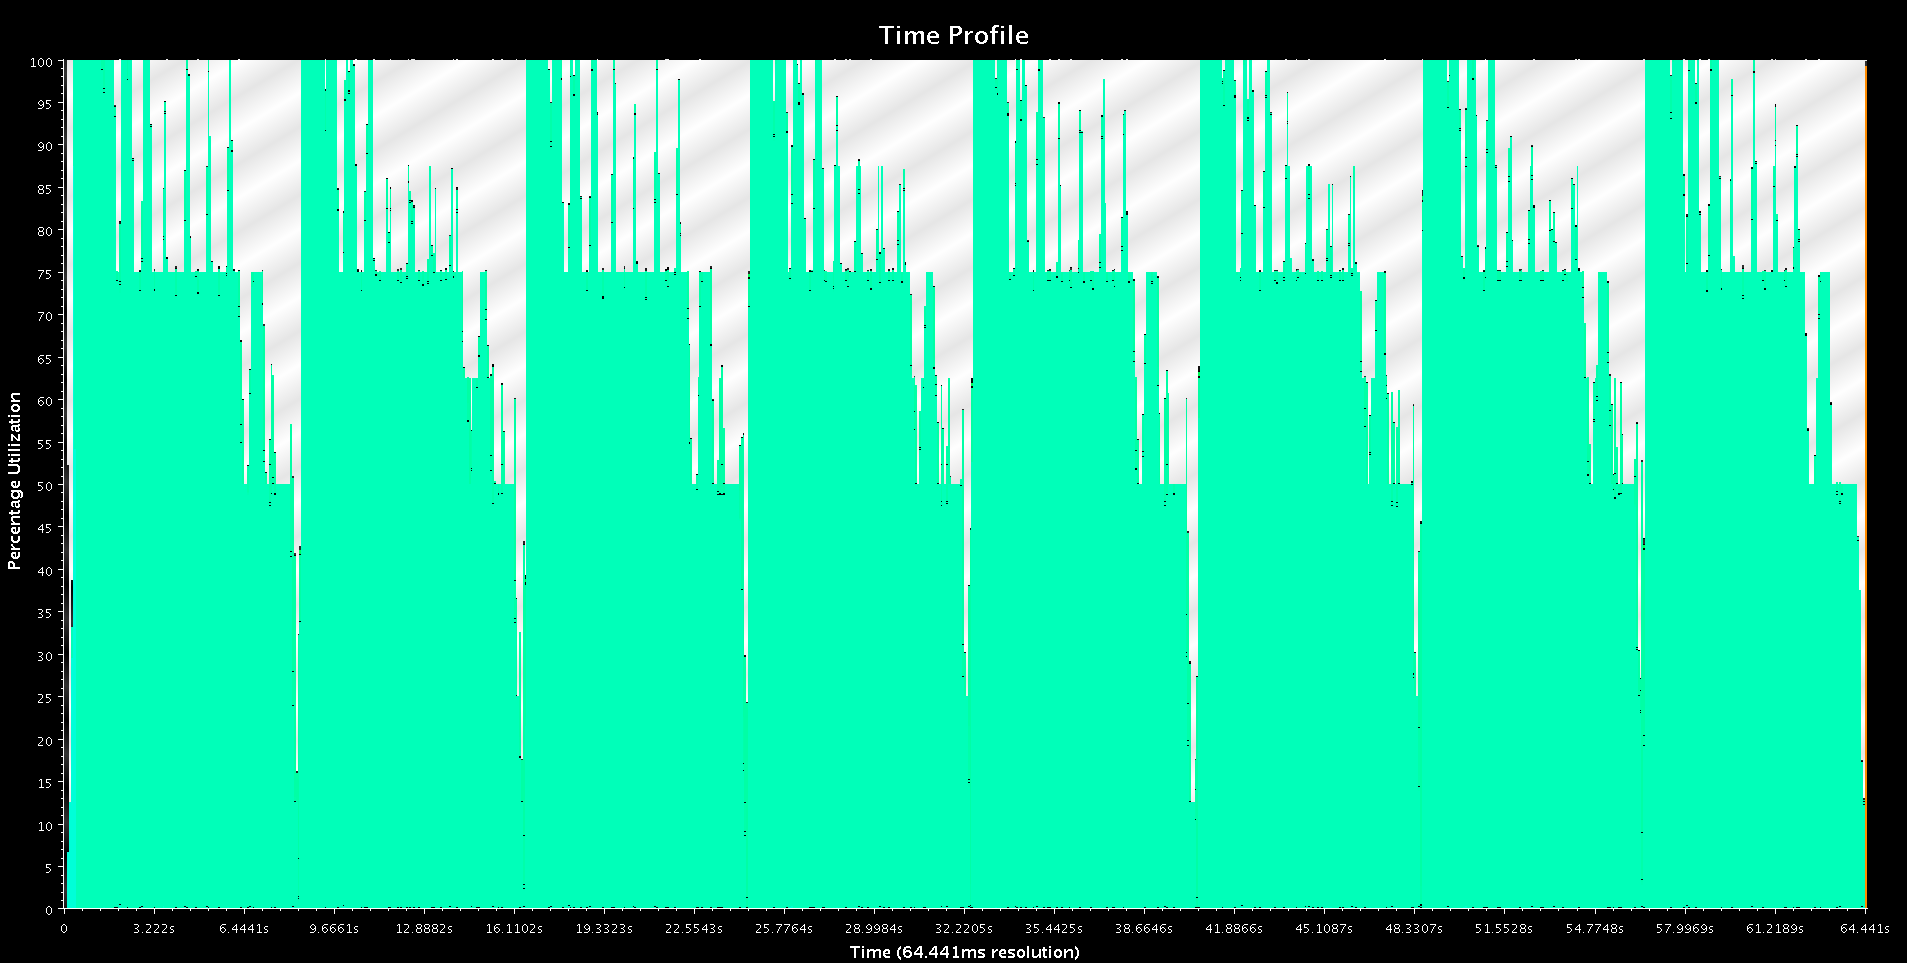
\includegraphics[width=.75\paperwidth,height=.27\paperheight]{figures/LoadBalancing/TimeProfileDummyLB}
    \caption{Time Profile}
  \end{figure}
  \begin{figure}
    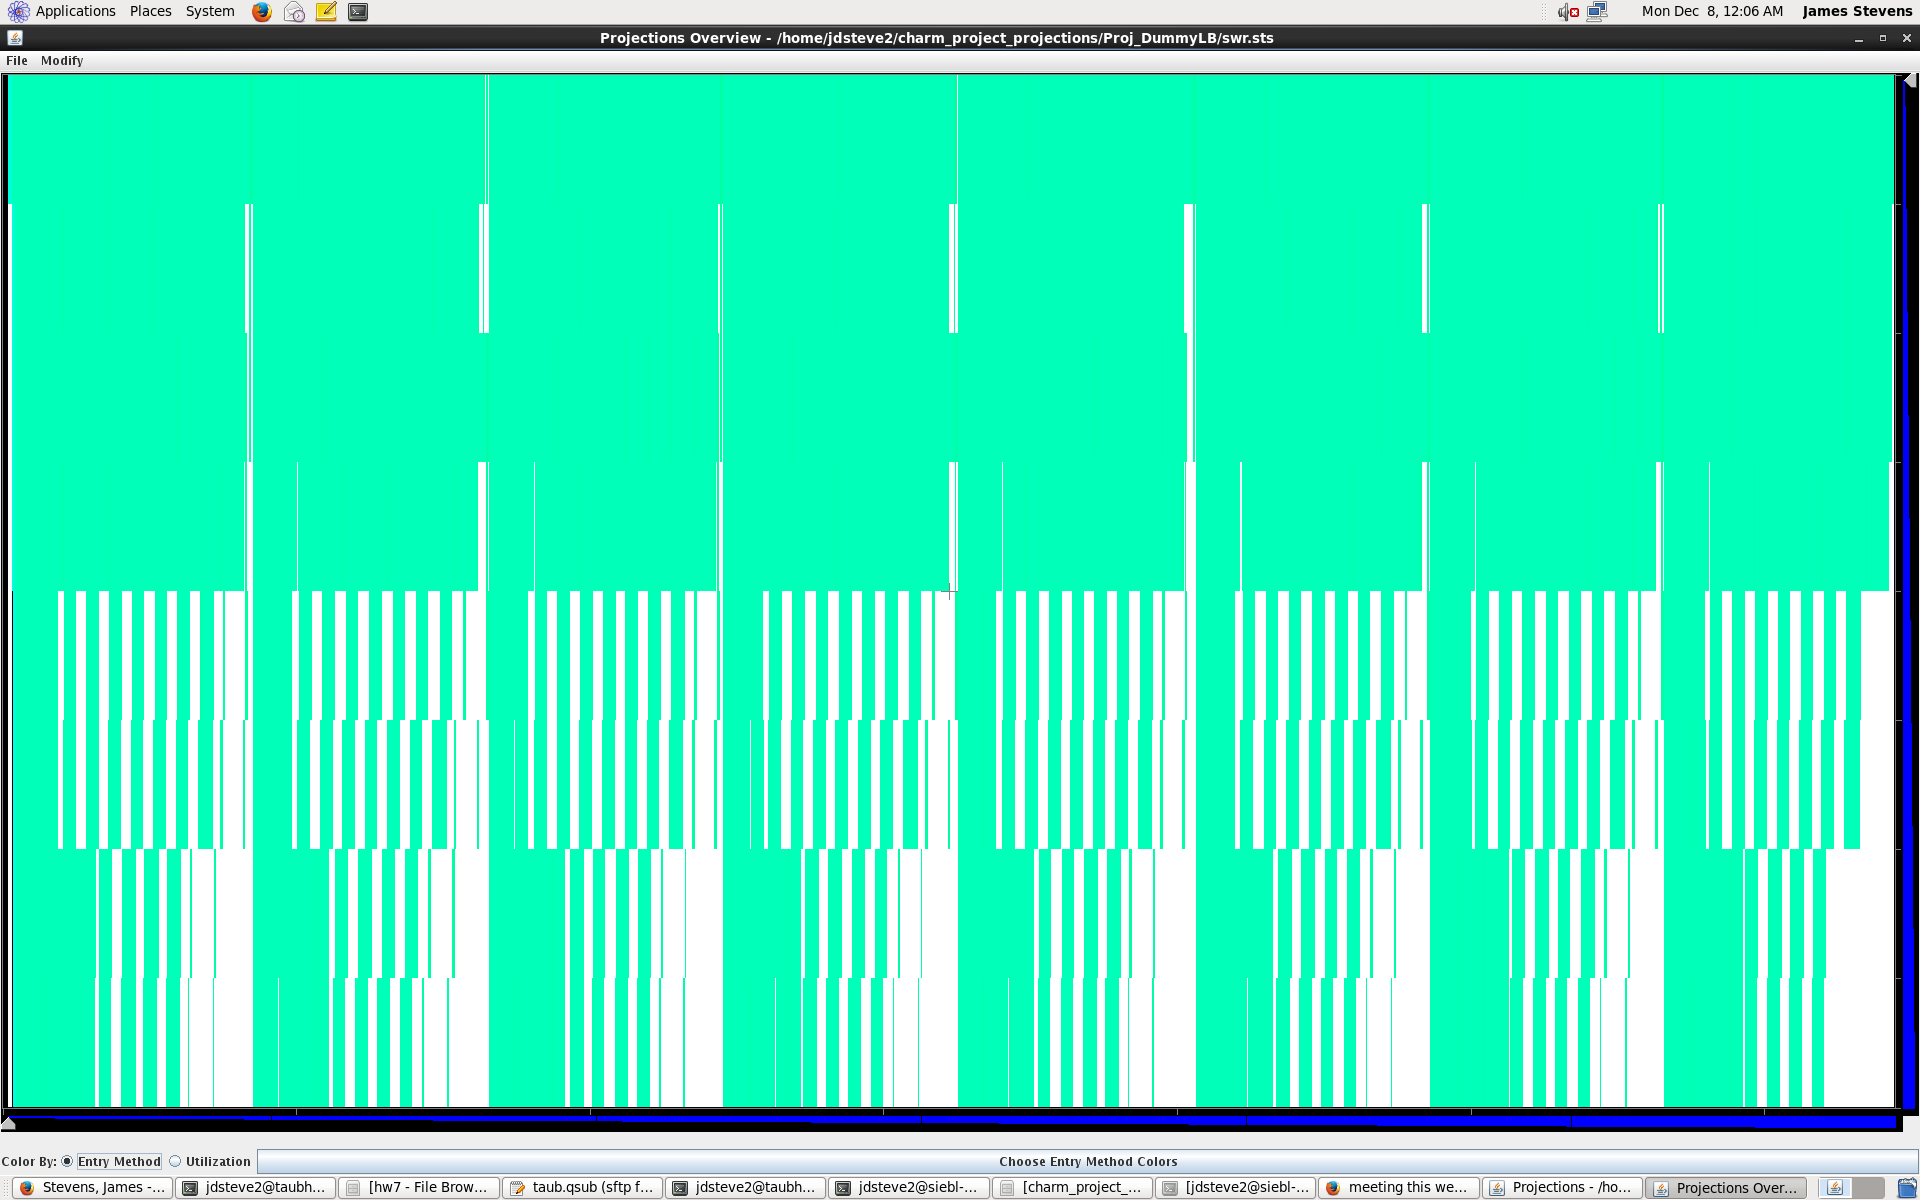
\includegraphics[width=.75\paperwidth,height=.27\paperheight]{figures/LoadBalancing/OverviewDummyLB}
    \caption{Core Overview}
  \end{figure}
\end{frame}

\begin{frame}{Numerical Experiments}{GreedyLB}
  \begin{figure}
    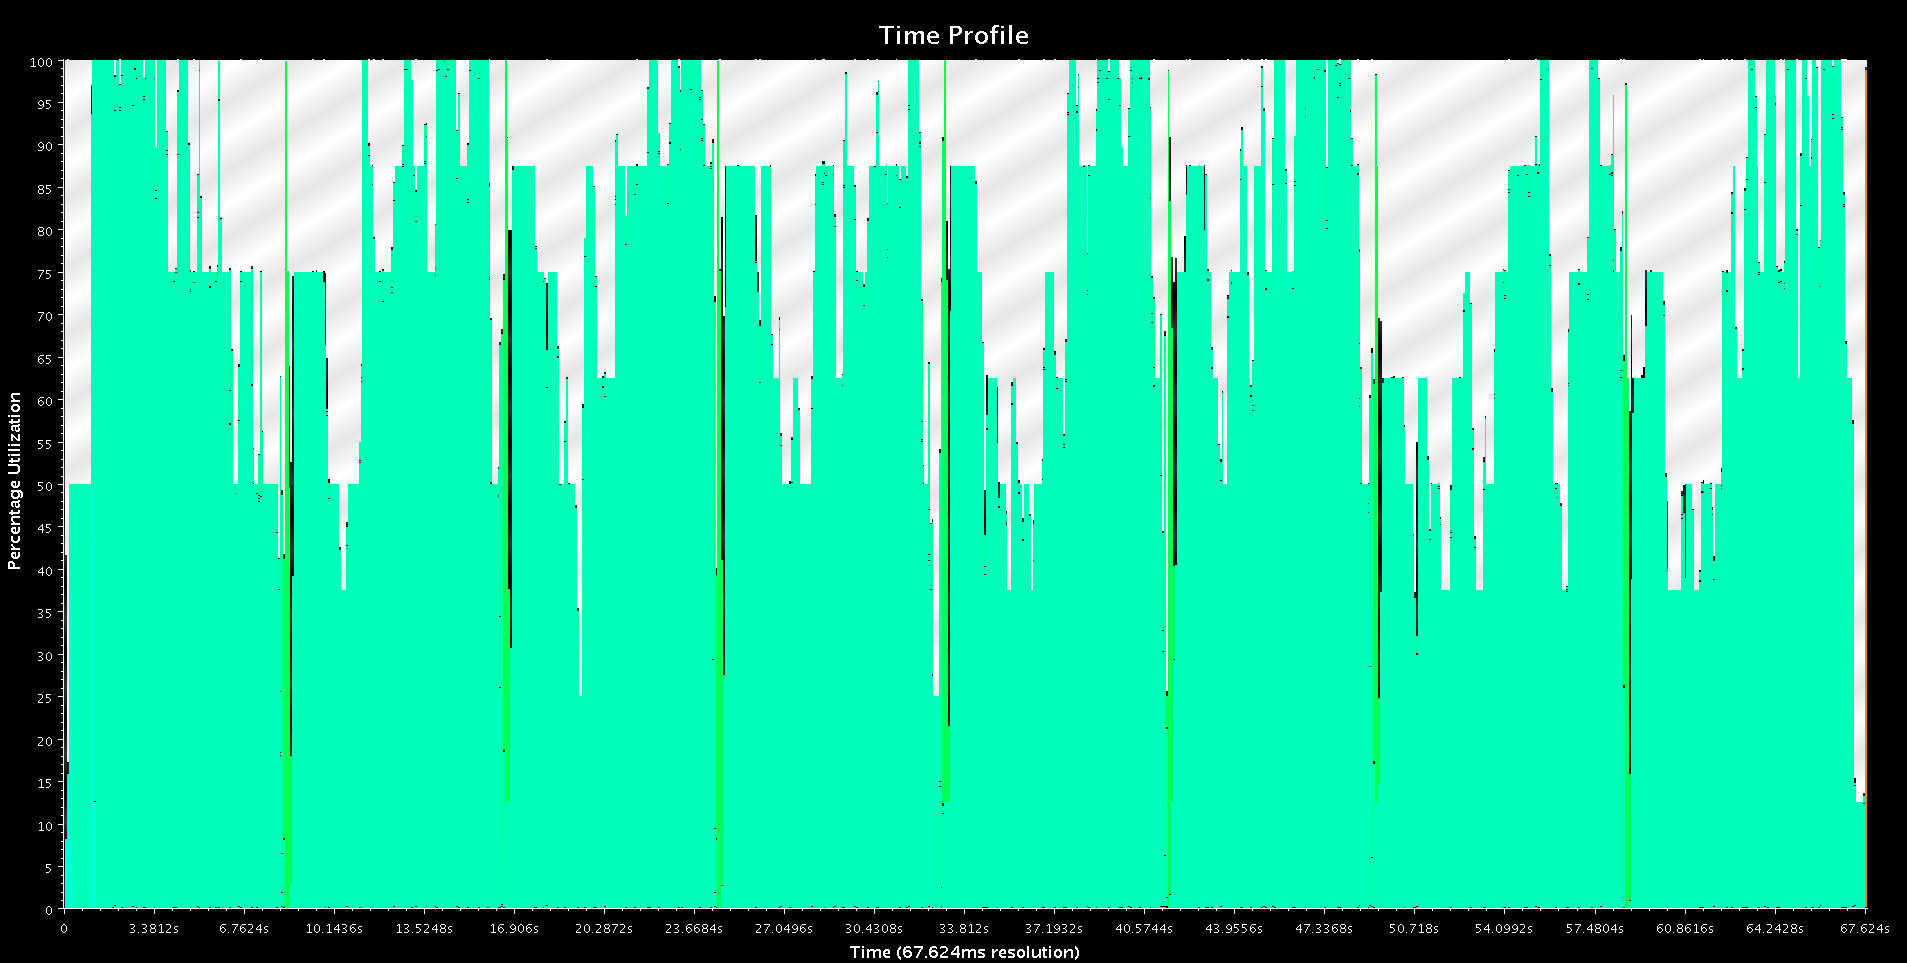
\includegraphics[width=.75\paperwidth,height=.27\paperheight]{figures/LoadBalancing/TimeProfileGreedyLB}
    \caption{Time Profile}
  \end{figure}
  \begin{figure}
    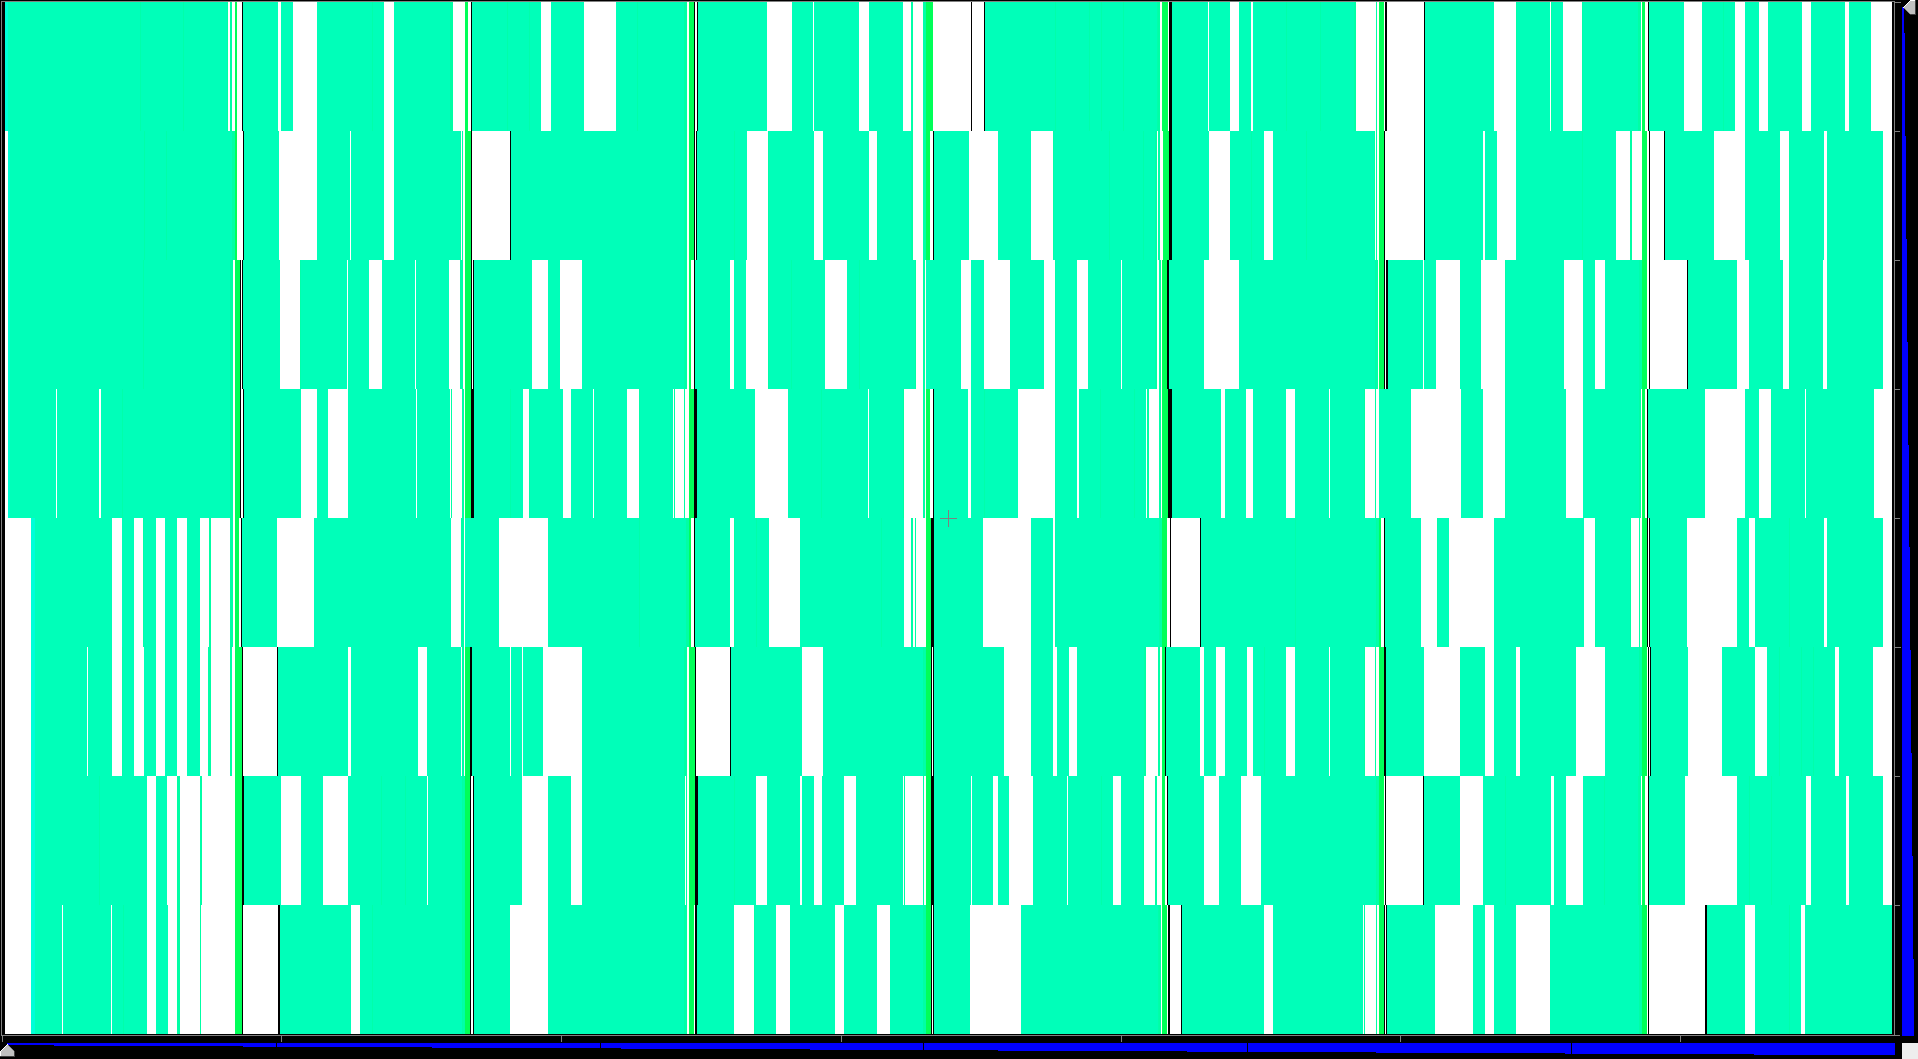
\includegraphics[width=.75\paperwidth,height=.27\paperheight]{figures/LoadBalancing/OverviewGreedyLB}
    \caption{Core Overview}
  \end{figure}
\end{frame}

\begin{frame}{Numerical Experiments}{RefineLB}
  \begin{figure}
    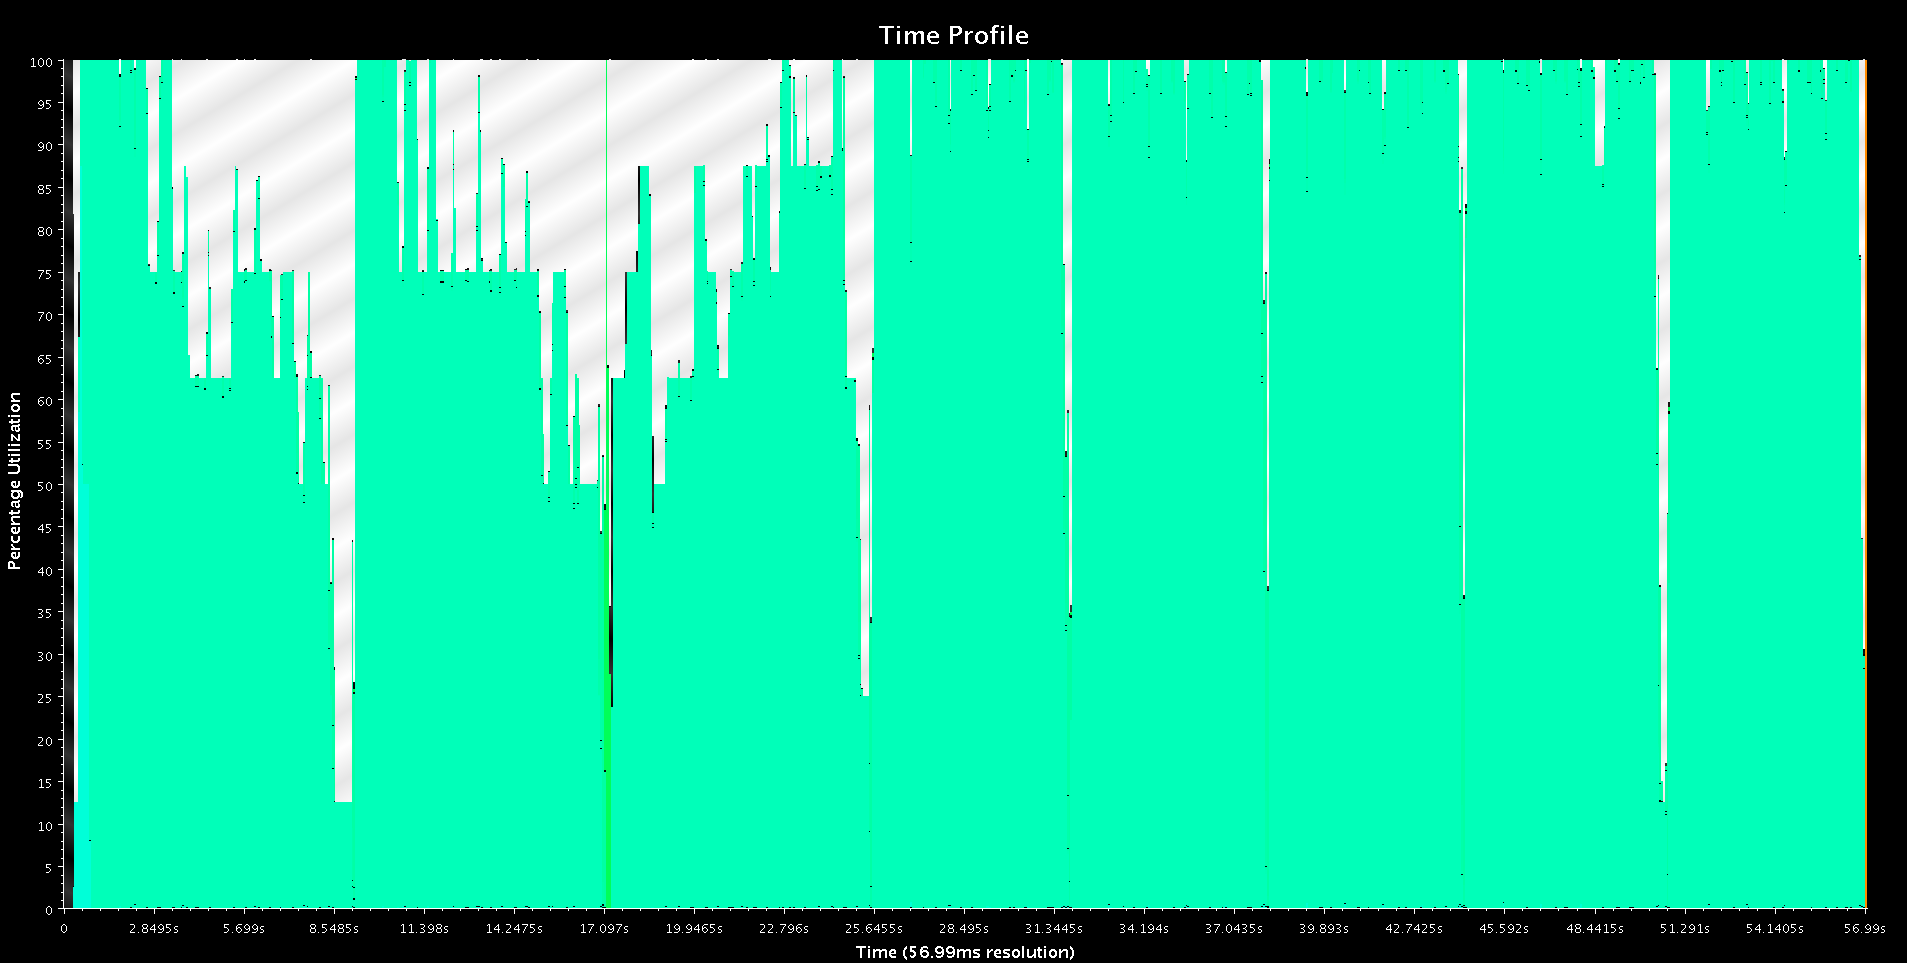
\includegraphics[width=.75\paperwidth,height=.27\paperheight]{figures/LoadBalancing/TimeProfileRefineLB}
    \caption{Time Profile}
  \end{figure}
  \begin{figure}
    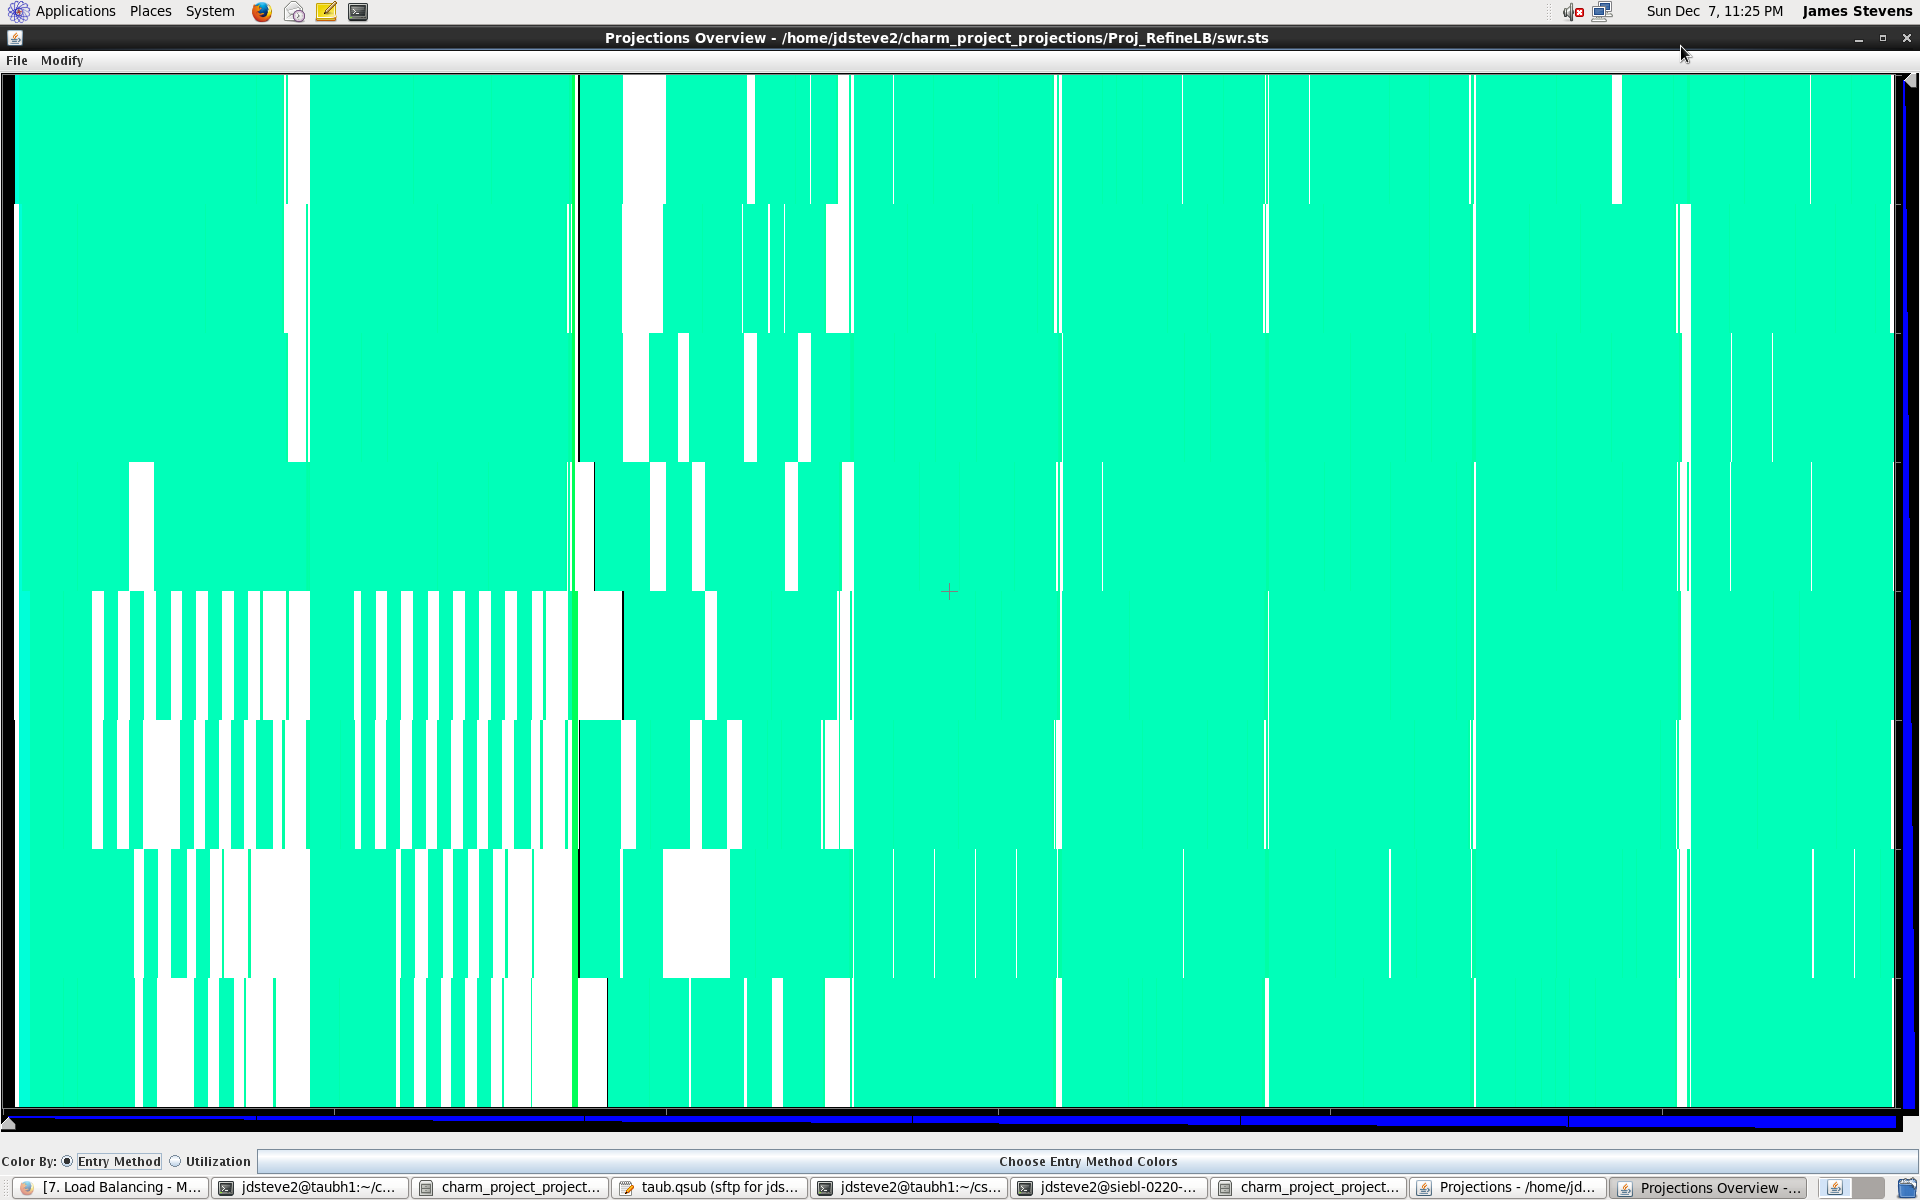
\includegraphics[width=.75\paperwidth,height=.27\paperheight]{figures/LoadBalancing/OverviewRefineLB}
    \caption{Core Overview}
  \end{figure}
\end{frame}

\section{Conclusion}

\begin{frame}{Future Work}

  \begin{itemize}
  \item PSWR
  \item Fully time adaptive SWR and PSWR
  \item Multiphysics
  \item Applications
  \end{itemize}

\end{frame}

\begin{frame}
  \frametitle{The End}
  \begin{center}
    \usebeamerfont*{frametitle} 
    Thank You!

    Questions / Comments?
  \end{center}
\end{frame}

\end{document}
